\documentclass[12pt, a4paper]{article}
\usepackage[T2A]{fontenc}
\usepackage[utf8]{inputenc}

\usepackage{fancyhdr} 
\usepackage{lastpage}
\usepackage{graphicx}
\usepackage{amsmath}
\usepackage{amsthm}
\usepackage{amsfonts}
\usepackage{amssymb}
\usepackage{xcolor}
\usepackage{bbm}
\usepackage{ulem}
\usepackage{wasysym}
\usepackage{bbold}
\usepackage{dsfont}
\usepackage{amsfonts}
\usepackage{wrapfig}
\usepackage[english,russian]{babel} 
\usepackage{chngcntr}
\usepackage[left=2.3cm, right=2.3cm, top=2.7cm, bottom=2.7cm, bindingoffset=0cm, headheight=15pt]{geometry} 
\usepackage[colorlinks=true,linkcolor=blue]{hyperref}
\usepackage{draftwatermark}
\SetWatermarkText{В матане как на войне}
\SetWatermarkScale{2}
\SetWatermarkColor[gray]{0.9}
% \usepackage{lmodern}

\usepackage{background}
\usepackage{etoolbox}
\usepackage{keystroke}

\makeatletter
\patchcmd{\tableofcontents}{\@starttoc{toc}}{\hypertarget{totoc}{}\@starttoc{toc}}{}{}
\makeatother

\backgroundsetup{
scale=1,
angle=0,
color=black,
position=current page.south,
vshift=20pt,
contents={
  \tikz[remember picture,overlay]
    \node[inner sep=0pt] {\hyperlink{totoc}{\Return}};
  }
}

\renewcommand{\footrulewidth}{0.4pt}
% \setlength{\parindent}{0em}
% \setlength{\parskip}{1em}

\pagestyle{fancy}
\rfoot{\thepage\ из \pageref{LastPage}}
\cfoot{}

\newcommand{\bnd}{\\[1ex]}
\newcommand{\Bnd}{\\[2ex]}
\newcommand{\RomanNum}[1]{\MakeUppercase{\romannumeral #1}}
\newcommand{\eqdef}{\stackrel{\mathrm{def}}{=}}
\newcommand{\scalar}[1]{\langle #1 \rangle}
\newcommand{\abs}[1]{\left| #1 \right|}

\DeclareMathOperator*{\xor}{\oplus}
\DeclareMathOperator*{\bigxor}{\bigoplus}
\DeclareMathOperator*{\R}{\mathbb{R}}
\DeclareMathOperator*{\Q}{\mathbb{Q}}
\DeclareMathOperator*{\Z}{\mathbb{Z}}
\DeclareMathOperator*{\B}{\mathbb{B}}
\DeclareMathOperator*{\N}{\mathbb{N}}
\DeclareMathOperator*{\0}{\mathbb{0}}
\DeclareMathOperator*{\1}{\mathbb{1}}
\renewcommand{\Vec}{\overrightarrow}
\renewcommand{\U}{\mathbb{U}}
\renewcommand{\C}{\mathbb{C}}

\theoremstyle{plain}
\newtheorem{theorem}{Теорема}
\newtheorem*{theorem*}{Теорема}
\newtheorem{axiom}{Аксиома}
\newtheorem{lemma}{Лемма}
\counterwithin*{theorem}{subsection}
\counterwithin*{axiom}{subsection}
\counterwithin*{lemma}{subsection}

\theoremstyle{definition}
\newtheorem*{definition}{Определение}

\theoremstyle{remark}
\newtheorem*{remark}{Примечание}
\newtheorem*{exercise}{Упражнение}
\newtheorem*{consequence}{Следствие}
\newtheorem*{example}{Пример}

\newcommand{\candle}{\ensuremath{\accentset{\scalebox{.5}{\(\varspadesuit\)}}{\scalebox{.6}{\(\talloblong\)}}}}

\title{\textbf{В матане как на войне} \\ Учебное пособие о том как затащить у Кохася К. П.}
\lhead{}

% Впиши сюда себя. Страна должна знать своих героев!
\author{ 
    @irdkwmnsb - Альжанов Максим   \\%
    @JelluSandro - Никита Шемякин   \\%
    @Dalvikk - Владислав Ковальчук   \\%
    @Turukmokto - Евгений Бессоницын  \\%     0
    @Onexx7 - Илья Зайцев              \\%  -- \ --
    @NULL3301 - Вадим Нагибин           \\%    / \
    @DimaUtyuz - Дмитрий Утюжников       \\%
    @RahimHakimov - Рахим Хакимов         \\%
    @Shady712 - Данил Крайнов              \\%
    @Moroness - Михаил Галибов              \\%
    @abramkht - Хетаг Дзестелов              \\%
    @whicha - Иван Алексеев                   \\%
    @maksimShekhunov - Максим Шехунов          \\%
}

\date{December 2020}

\begin{document}
% \fontfamily{lmss}\selectfont
\maketitle

\newpage
\tableofcontents

\newpage
\section*{Как это редактировать?}

Таблицу можно сделать так: \\
Распределение вариантов \\ 
\begin{tabular}{|c|c|} \hline 
     Строчки в табличке Кохася & Кто \\ \hline 
    3 -- 7 & Шемякин \\ \hline 
    8 -- 12 & Зайцев \\ \hline 
    13 -- 17 & Бессонницын \\ \hline 
    18 -- 22 & Крайнов \\ \hline 
    23 -- 27 & Ковальчук \\ \hline 
    28 -- 32 & Утюжников \\ \hline 
    33 -- 37 & Нагибин \\ \hline  
    38 -- 42 + 59 & Алексеев \\ \hline 
    43 -- 47 + 60 & Галибов \\ \hline 
    48 -- 52 + 61 & Хакимов \\ \hline 
    53 -- 57 + 62 & Дзестелов \\ \hline 
\end{tabular}

Формулы вы делать умеете, АИСД сдаете же как-то

Картинки можно вставлять так: \\
% scale --- масштабирование. Подробнее в интернете

\includegraphics[scale = 0.5]{Images/smile.jpeg}

Внизу в левом углу вы видите File outline, в нем содержатся ссылки на заголовки, чтобы можно было быстро перейти к своей части \\
\textbf{Пожалуйста, следите за тем чтобы после вашего кода не возникало кучу ошибок при компиляции!} \\
Если что то похерилось --- писать Владу или Максиму (@Dalvikk, @irdkwmnsb) \\
    $a \ b$  --- маленький пробел в режиме набора мат формул \\
    $a \quad b$   --- средний \\ 
    $a \qquad b$  --- большой \\

Лайфхак: дважды нажмите на текст в пдфке и ваш курсор переместится на ее латех код

Комент

Как написать комент: В правом верхнем углу есть кнопка Review, после ее нажатия откроется поле где видны комментарии + выделив текст можно можно добавить новый тыкнув на Add comment
\newpage
\section{Теоремы}
% Так как нумерация строк в табличке Кохася с 3
\setcounter{subsection}{2}

\rhead{Шемякин}
\subsection{Законы Де Моргана}
	
	\begin{theorem*}
		\begin{equation}
			Y \setminus\left(\bigcup\limits_{\alpha \in A} X_\alpha \right) = \bigcap\limits_{\alpha \in A} \left( Y \setminus X_\alpha \right) 
		\end{equation}
		
		\begin{equation}
			Y \setminus\left(\bigcap\limits_{\alpha \in A} X_\alpha \right) = \bigcup\limits_{\alpha \in A} \left( Y \setminus X_\alpha \right) 
		\end{equation}
		
		\begin{equation}
			Y \bigcap \left(\bigcup\limits_{\alpha \in A} X_\alpha \right) =  \bigcup\limits_{\alpha \in A} \left(Y \bigcap X_\alpha \right)
		\end{equation}
		
		\begin{equation}
			 Y \bigcup \left(\bigcap\limits_{\alpha \in A} X_\alpha \right) =  \bigcap\limits_{\alpha \in A} \left(Y \bigcup X_\alpha \right)
		\end{equation}
	\end{theorem*}
	
	\begin{proof}
		 Докажем (1), остальные аналогично (см. фото)
		 $$ x \in \text{левой части} \Leftrightarrow (x \in Y) \text{ и } \left(x \notin \bigcup\limits_{\alpha \in A} X_\alpha \right) \Leftrightarrow x \in Y \text{ и } \forall \alpha \in A \ \ x \notin X_\alpha \Leftrightarrow $$  $$ \Leftrightarrow \forall \alpha \in A ~ \left(x \notin X_\alpha \text{ и } x \in Y \right) \\ \Leftrightarrow  \forall \alpha \in A \ \ x \in (Y \setminus X_\alpha) \Leftrightarrow \bigcap\limits_{\alpha \in A} \left (Y \setminus X_\alpha \right) $$
	\end{proof}
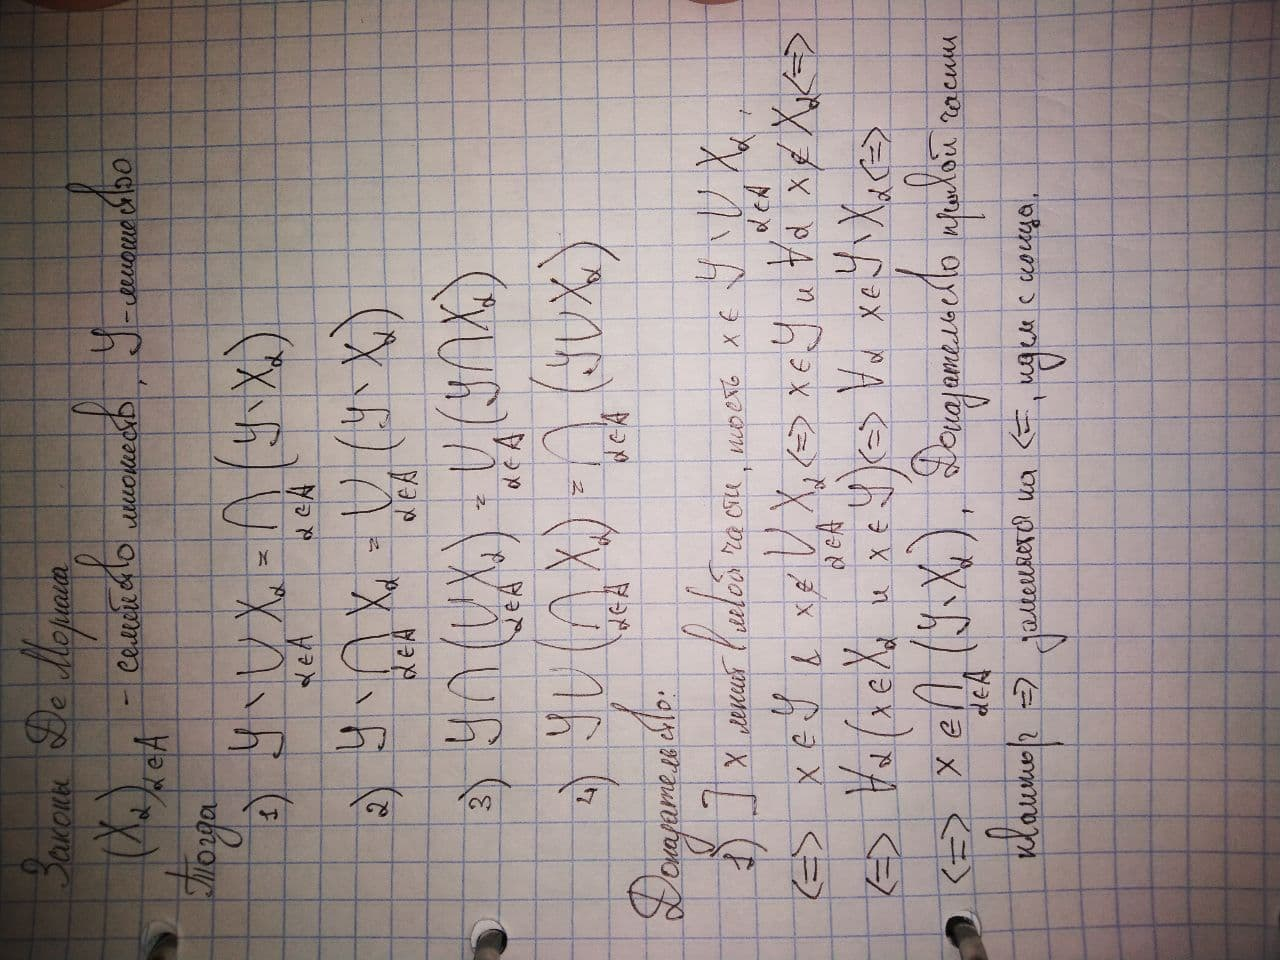
\includegraphics[height = 0.7\textheight, width = \textwidth]{Images/законы деморгона.jpg}
% Вроде норм получилось

% к сожалению в латексе нет значков для записи объедение по альфа
% к счастью есть :)
% $\bigcup\limits_{\alpha \in A} G_\alpha$

% поэтому вот вам картинки, слов тут все равно не много
%как кстати нормально картинки встасить

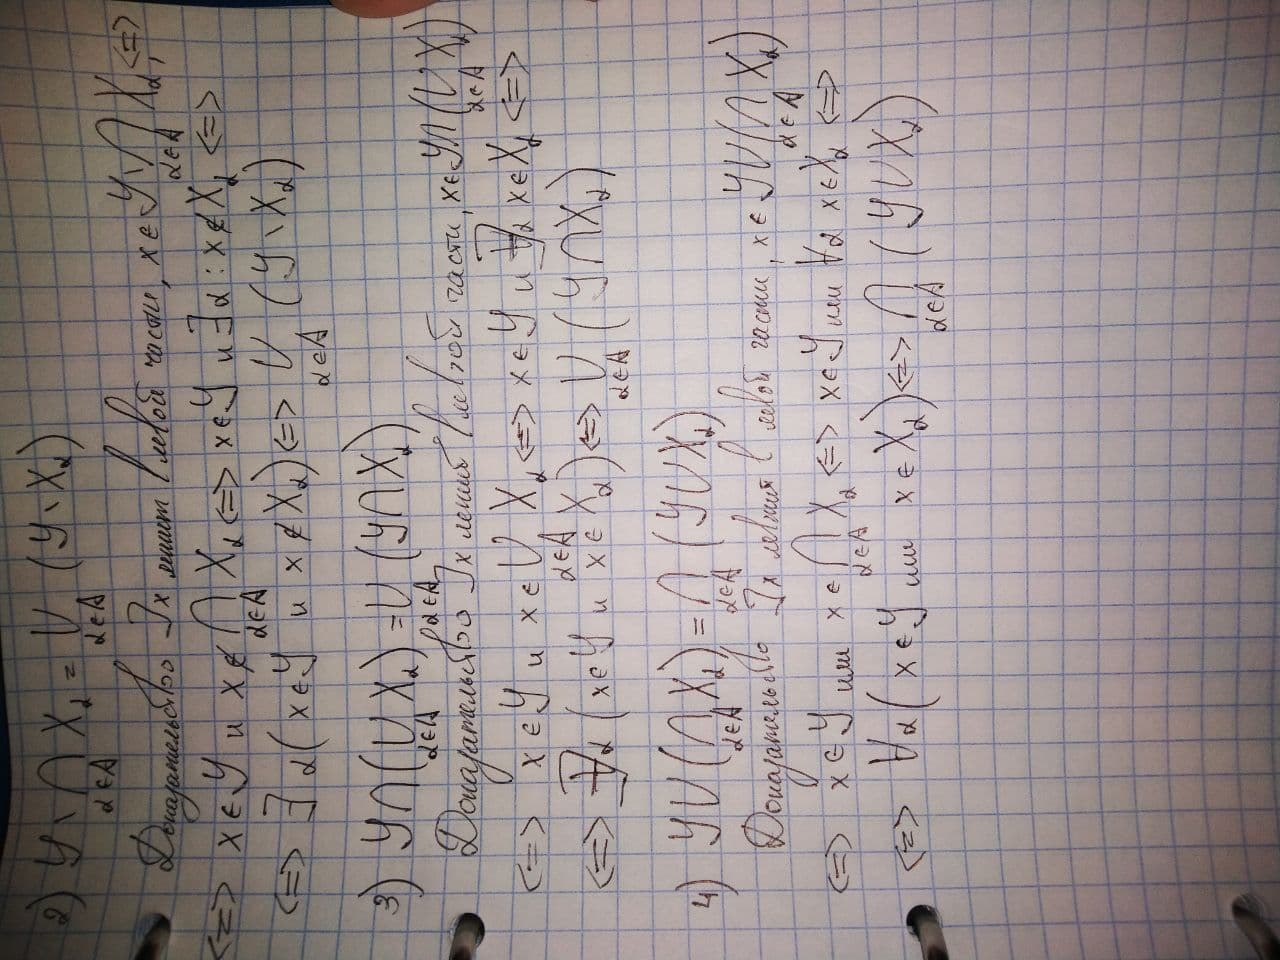
\includegraphics[width =\textwidth, height = 0.8\textheight]{Images/доказательства де моргана.jpg}
% Вроде норм получилось

%техать мы это не будем по причине кванторы

% ленивая жопа

\newpage
\subsection{Единственность предела и ограниченность сходящейся последовательности}
\begin{definition}
     Последовательность $ { ( {x_{n}} )_{n \varepsilon  {N} }}$ - семейство, заиндексированное натуральными числами.
\end{definition}

    %  ${x_{n}}\varepsilon  R$ 
     
    %  Пусть есть $ { ( {x_{n}} )_{n \varepsilon  {N} }}$ и $a \varepsilon  R$
     
    % $ {x_{n}} \rightarrow a$ 
    
    % $\lim\limits_{n \to \infty} x_n = a$
    
    % %как в формулы пробела вставить а       
    
    % $\forall \varepsilon > 0 \ \exists N \  \forall n > N: \abs{{x_{n}} - a} < \varepsilon$ \\
    
    % (Расстояние от ${x_{n}}$ до $a$) $< \varepsilon \Leftrightarrow \abs{{x_{n}} - a} < \varepsilon$ 
    
    % Примеры:
    % \begin{enumerate}
    %     \item ${x_{n}}$ - стационарная последовательность $x_n = a$ 
        
    %     $\lim\limits_{n \to \infty} x_n = a$
        
    %     \item $x_n = \frac{1}{n}$ тогда $x_n \longrightarrow 0$
        
    %     $\forall \ \varepsilon > 0 \  \exists N = \frac{1}{\varepsilon} \ \forall \  n > \frac{1}{\varepsilon} \ \ \frac{1}{n} < \varepsilon$
        
    %     \item $x_n = (-1)^{n}$ Расходится
        
    %     $\forall \ \varepsilon > 0 \  \exists N  \ \forall \  n > N \ \ \abs{x_n - a} < \varepsilon$
        
    %     заменим $N$ на $N(\varepsilon)$ N от епсилон. Тогда $ \forall n > N(\varepsilon) \  \abs{x_n - a} < \varepsilon$
        
    %     Тоесть $(N(\varepsilon); \infty)$
        
    %     Тогда рассмотрим для конкретного $\varepsilon = 1 \ \exists N(1) \ \forall \ n > N(1) \ \ \abs{x_n - a} < 1$
        
    % \end{enumerate}
    % \quad
    \begin{theorem*} (О единственности предела)
        $x_n$- последовательность в метрическом пространстве $(X, \rho)$
        
        $a, b \in X$, $x_n \to a$, $x_n \to b \Rightarrow a = b$
    \end{theorem*}
    
    \begin{proof}
        Предположим $a \neq b$, следовательно существуют окрестности точек $a$ и $b$, что они не пересекаются: 
        
        $U(a) = B_1(a, \frac{1}{2}r) \ \ \ \ V(b) = B_2(b, \frac{1}{2}r)$ 
        
        $r = \rho(a,b)$
        
        Докажем от противного, что эти шары  $B_1$  и $B_2$ не пересекаются.
        
        Пусть $z \in B_1$ и $z \in B_2$ - точка пересечения
        
        $\rho(a, z) < \frac{1}{2} r$
        
        $\rho(b, z) < \frac{1}{2} r$
        
        $\rho(a, b) = r > \rho(a, z) + \rho(z, b)  \Rightarrow \frac{1}{2}r + \frac{1}{2}r < r$ {---} противоречие по неравенству треугольников $\Rightarrow$ шары не пересекаются
         
        Рассмотрим непересекающиеся окрестности $U(a), V(b)$. Вне $U(a)$ конечное число членов последовательности $\Longrightarrow$ в $V(b)$ конечное число членов последовательности. Получили противоречие.
    \end{proof}
    
    \begin{theorem*} (Об ограничености сходящейся последовательности)
        В метрическом пространстве сходящаяся последовательность ограниченна.
        
        Последовательность $x_n$ ограниченна, если множество ее значений ограниченно.
    \end{theorem*}
    \begin{proof}
        Для $\varepsilon = 1 \ \ \exists N \ \forall n > N \ \ q(x_n, a) < 1$ определение предела для $\varepsilon = 1$
        
        $R = max(q(x_i, a))$ Берем конечные точки и раширяем шар до максимального среди них радиуса. Откуда $x_n \subset B(a, R)$.
    \end{proof}
    
\newpage
\subsection{Теорема о предельном переходе в неравенствах для последовательностей и для функций}
    \begin{theorem*}
    $x_n , y_n$ - вещественные последовательности.
    
    $a, b \in X$, $x_n \to a$, $x_n \to b$. Если $\forall n \in N \ \ x_n \leqslant y_n \Rightarrow a \leqslant b$.
    \end{theorem*}
    \begin{proof}
    Докажем от противного.
    
    Пусть $b < a$
    
    $\varepsilon = \frac{a - b}{2}$ растояние от $a$ до $b \Rightarrow b + \varepsilon = a - \varepsilon$
    
    Для этого же $\varepsilon \ \ \exists \ \ N_1 \ \ \forall n > N_1 \abs{x_n - a} < \varepsilon \Rightarrow a - \varepsilon < x_n$
    
    Для этого же $\varepsilon \ \ \exists \ \ N_2 \ \ \forall n > N_2 \abs{y_n - b} < \varepsilon \Rightarrow y_n < b + \varepsilon$ 
    
    Тогда при $n > max(N_1, N_2)$
    
    $y_n < b + \varepsilon = a - \varepsilon < x_n$ 
    
    $y_n < x_n$ {---} противоречие
    \end{proof}
    
    \begin{remark}
        $x_n = -\frac{1}{n} \ \ y_n = \frac{1}{n} \ \ x_n < y_n$
        
        Знак не может быть строгим $ 0 \leqslant 0$
        
        Верны варианты теорем с одной последовательностью $\forall n \ x_n \leq b$
        
        $x_n \to a$
        
        Тогда $a \leqslant b$
        
        Если $x_n \in [a; b]$, $x_n \longrightarrow \alpha$ тогда $\alpha \in [a; b]$
    \end{remark}
\newpage
\subsection{Теорема о двух городовых}
\begin{theorem*}
    Пусть есть 3 последовательности $(x_n), (y_n), (z_n)$ - вещественные последовательности
    
    $\forall \ n \ x_n \leqslant y_n \leqslant z_n$ Пусть $x_n \longrightarrow a, z_n \longrightarrow a$
    Тогда, $\exists$ предел $\lim\limits_{n \to \infty} y_n$ и это предел $\lim\limits_{n \to \infty} y_n = a$
\end{theorem*}
\begin{proof}
    $\forall \ \ \varepsilon > 0 \ \ \exists N_1 \ \ \forall \ \ n > N_1 \ \ \ \abs{x_n - a} < \varepsilon \Rightarrow a - \varepsilon < x_n$
    
    $\forall \ \ \varepsilon > 0 \ \ \exists N_2 \ \ \forall \ \ n > N_2 \ \ \ z_n < a + \varepsilon$
    
    $N = max(N_1, N_2), \forall n > N$
    
    $a - \varepsilon < x_n \leqslant y_n \leqslant z_n < a + \varepsilon$
    
    $a - \varepsilon < y_n < a + \varepsilon$
\end{proof}
\begin{remark}
    $\forall n \ \ x_n < y_n$ и $x_n \leqslant y_n \leqslant z_n$
    
    $\exists \ \ k \ \ \forall n > k$ неравенство с некоторго номера k выполняется
    
    Частный случай $(x_n), (y_n), \forall \ \ n \ \ \abs{x_n} \leqslant y_n $ и $y_n \longrightarrow 0$
    
    Тогда $x_n \longrightarrow 0$, $-y_n \leqslant x_n \leqslant y_n$, $y_n \longrightarrow 0$, $-y_n \longrightarrow 0$
    
    Для комплексного $x_n$ и $y_n \in R$, $Re(x_n) \leqslant \abs{x_n} \leqslant y_n$
    
    $-y_n \leqslant -\abs{x_n} \leqslant Re(x_n) \leqslant \abs{x_n} \leqslant y_n$
\end{remark}
\newpage
\subsection{Бесконечно малая последовательность}
    Вещественная последовательность, называется бесконечно малой, если она стремится к 0, т. е. $x_n \longrightarrow 0$
    
    \begin{remark}
        Бесконечно малых чисел не бывает (Аксиома Архимеда), поэтому записать стремление к нулю в предыдущих терминах не очень содержательно.
    \end{remark}
    \begin{theorem*}
    
    $(x_n), (y_n)$ {---} вещественные последовательности
    
    $x_n$ {---} бесконечно малая, $y_n$ {---} ограниченная
    
    Тогда $z_n = x_n \cdot y_n$ бесконечно малая.
    \end{theorem*}
    \begin{proof}
    $\exists M \  \forall n \ \abs{y_n} \leqslant M $, так как $y_n$ - ограниченна.
    
    $\forall \varepsilon > 0 \ \exists N  \ \forall n > N \ \abs{x_n} < \varepsilon$
    заменяем на
    $\abs{x_n \cdot y_n} < M  \varepsilon$
      
    $\forall \varepsilon > 0 \ \exists N \ \forall n > N \ \abs{x_n}\cdot\abs{y_n} = \abs{z_n} < M\varepsilon $ 
    
    Заменим $\varepsilon' = \frac{\varepsilon}{M}$ (Китайский фокус)
    
    Тогда $\forall \varepsilon' \ \exists N \ \ \forall n > N \ \abs{z_n} < \varepsilon'$
    
    %Как же я заебался это техать
    
    \end{proof}
\newpage
\rhead{Зайцев}
\subsection{Теорема об арифметических свойствах предела последовательности в нормированном пространстве и в $\R$} %1:07(5-6)
  
\begin{theorem*}{Об арифметических свойствах предела последовательности в нормированном пространстве.} 

    Пусть даны:
  
    $(X, ||\cdot||)$ --- нормированное пространство
    
    $(x_n), (y_n)$ --- последовательности элементов $X$
    
    $\lambda_n$ --- последовательность скаляров    $x_n\rightarrow x, y_n\rightarrow y, \lambda_n\rightarrow \lambda, x \in X, y \in X, \lambda \in \R(\C)$
    
    Тогда утверждается нескольство свойств:
    \begin{enumerate}
    \item $x_n \pm y_n \rightarrow x \pm y$
    \item $\lambda_n x_n \rightarrow \lambda x$
    \item $||x_n|| \rightarrow ||x||$
    \end{enumerate}
\end{theorem*}

\begin{proof} $ $
\begin{enumerate}
\item $\forall \varepsilon > 0$\\
$\exists N_1 \ \forall n > N_1 \quad ||x_n - x|| < \frac{\varepsilon}{2}$\\
$\exists N_2 \ \forall n > N_2 \quad ||y_n - y|| < \frac{\varepsilon}{2}$\\
Тогда при $n > max(N_1, N_2)$ выполняется\\
$||x_n + y_n - (x + y)|| \leq ||x_n - x|| + ||y_n - y|| < \frac{\varepsilon}{2} + \frac{\varepsilon}{2} = \varepsilon$
\item $||\lambda_n x_n - \lambda x|| = ||(\lambda_n x_n - \lambda_n x) + (\lambda_n x - \lambda x)|| \leq ||\lambda_n (x_n - x)|| + ||(\lambda_n - \lambda) x|| = |\lambda_n|\cdot ||x_n - x|| + |\lambda_n - \lambda|\cdot ||x||$\\
$|\lambda_n|$ --- ограничено\\
$||x_n - x||$ --- бесконечно малое\\
$|\lambda_n - \lambda|$ --- бесконечно малое\\
$||x||$ --- ограничено\\
б.м. $\cdot$ огр. + огр. $\cdot$ б.м. $\Rightarrow$ все выражение бесконечно малое по теореме о бесконечно малой последовательности (пункт 1.7)
\item $\Big|||x_n|| - ||x||\Big| \leq ||x_n - x|| \rightarrow 0$
\end{enumerate}
\end{proof}
\textbf{Арифметические свойства предела в $\R$}\\
$(x_n), (y_n)$ --- вещественные последовательности\\
$x_n\rightarrow x, y_n\rightarrow y, x \in \R, y \in \R$\\
Тогда утверждается нескольство свойств:
\begin{enumerate}
\item $x_n \pm y_n \rightarrow x \pm y$
\item $x_n y_n \rightarrow x y$
\item $|x_n| \rightarrow |x|$
\item Если $y \neq 0$ и $\forall n \ y_n \neq 0$ то $\frac{x_n}{y_n} \rightarrow \frac{x}{y}$
\end{enumerate}
$\R$ --- нормированное пространство, следовательно, 1-3 --- доказаны\\
Доказательство 4:\\
Заметим $\frac{x_n}{y_n} = x_n \cdot \frac{1}{y_n}$\\
Достаточно проверить $\frac{1}{y_n} \rightarrow \frac{1}{y}$ (далее по свойству 2)\\
$|\frac{1}{y_n} - \frac{1}{y}| = |y_n - y|\cdot |\frac{1}{y}| \cdot |\frac{1}{y_n}|$\\
$|y_n - y|$ --- бесконечно малое\\
$|\frac{1}{y}|$ --- ограничено\\
Докажем, что $|\frac{1}{y_n}|$ --- ограничено\\
$y_n \rightarrow y \neq 0$\\
Для $\varepsilon = |y| \cdot \frac{1}{2}\quad \exists N \ \forall n > N$\\
Для случая $y > 0$\\
$\frac{y}{2} < y_n < \frac{3}{2}y$\\
$\frac{2}{3y} < \frac{1}{y_n} < \frac{2}{y}$\\
В общем случае $|\frac{2}{3y}| < |\frac{1}{y_n}| < |\frac{2}{y}|$\\
Тогда число $M = max(\frac{1}{|y_1|}, \frac{1}{|y_2|} ... \frac{1}{|y_N|}, \frac{2}{|y|})+1$ --- верхняя граница последовательности $\frac{1}{y_n}$, т. е. $\forall n \in \N \ 0 \leq |\frac{1}{y_n}| \leq M$, следовательно, $\abs{\frac{1}{y_n}}$ ограничена.\\
Из этого следует, что $|\frac{1}{y_n} - \frac{1}{y}| = |y_n - y|\cdot |\frac{1}{y}| \cdot |\frac{1}{y_n}| \longrightarrow 0$, следвательно, $\frac{1}{y_n} \rightarrow \frac{1}{y}$, что и требовалось проверить.\\

\newpage
\subsection{Неравенство Коши-Буняковского в линейном пространстве, норма, порожденная скалярным произведением}
 %1:47(5-6)
 \textbf{Неравенство Коши-Буняковского в линейном пространстве}\\
$\forall x,y \ \ |\scalar{x,y}|^2 \leq \scalar{x,x}\scalar{y,y}$ --- нер-во Коши-Буняковского в линейном пространстве\\
Доказательство:\\
$0 \leq \scalar{x+ty,x+ty} = \scalar{x,x} + t \scalar{y,x} + \overline{t} \scalar{x,y} + t \cdot \overline{t}\scalar{y,y}$ по свойствам скалярного произведения.\\
Подставим $t = \frac{-\scalar{x,y}}{\scalar{y,y}}$ (при $y=0$ изначальное неравенство тривиально, рассматриваем $y \neq 0$)\\
$\scalar{x,x} - \frac{\scalar{x,y}\scalar{y,x}}{\scalar{y,y}} - \frac{\overline{\scalar{x,y}}\scalar{x,y}}{\scalar{y,y}} + \frac{\scalar{x,y}\scalar{y,x}}{\scalar{y,y}} = \scalar{x,x} - \frac{|\scalar{x,y}|^2}{\scalar{y,y}} \geq 0$ (пояснение: $\overline{\scalar{x,y}} = \scalar{y,x}$ и $\overline{\scalar{x,y}}\scalar{x,y} = |\scalar{x,y}|^2$)\\
Преобразуя финальное неравенство можно получить исходное $\Rightarrow$ доказано.\\
Пример:\\%возможно тут какая-то лажа
$\scalar{x,y} = x_1 y_1 + x_2 y_2 + ... + x_n y_n$\\
$(x_1 y_1 + x_2 y_2 + ... + x_n y_n)^2 \leq (x_1^2 + x_2^2 + ... + x_n^2)\cdot(y_1^2 + y_2^2 + ... + y_n^2)$\\
$\Leftrightarrow|x_1 y_1 + x_2 y_2 + ... + x_n y_n| \leq \sqrt{x_1^2 + x_2^2 + ... + x_n^2}\cdot \sqrt{y_1^2 + y_2^2 + ... + y_n^2}$\\
\textbf{Норма, порожденная скалярным произведением}\\
$X$ --- линейное пространство со скалярным произведением\\
Тогда функция $\rho(x) := \sqrt{\scalar{x,x}}$ - норма в $X$\\
Свойства нормы:
\begin{enumerate}
\item $\rho(x) \geq 0 \qquad \rho(x) = 0 \leftrightarrow x = 0$
\item $\rho(\alpha x) = |\alpha| \rho(x)$\\
Доказательство: $\rho(\alpha x) = \sqrt{\scalar{\alpha x, \alpha x}} = \sqrt{\alpha \overline{\alpha} \scalar{x,x}} = |\alpha| \rho(x)$
\item $\rho(x+y) \leq \rho(x) + \rho(y)$\\
Доказательство:\\
Возведем обе части в квадрат\\
$\scalar{x+y,x+y} \leq_? \scalar{x,x} + \scalar{y,y} + 2\sqrt{\scalar{x,x}\scalar{y,y}}$\\
Используем часть из доказательства неравенства Коши-Буняковского\\
$\scalar{x,y} + \scalar{y,x} + \scalar{x,x} + \scalar{y,y} \leq_? \scalar{x,x} + \scalar{y,y} + 2\sqrt{\scalar{x,x}\scalar{y,y}}$\\
Сокращаем\\
$\scalar{x,y} + \scalar{y,x} \leq_? 2\sqrt{\scalar{x,x}\scalar{y,y}}$\\
Верно по неравенству Коши-Буняковского\\
$2\operatorname{Re}\scalar{x,y} \leq 2 |\scalar{x,y}|  \leq 2\sqrt{\scalar{x,x}\scalar{y,y}}$
\end{enumerate}


\newpage
\subsection{Леммы о непрерывности скалярного произведения и покоординатной сходимости в $\R^n$} %2:04(5-6)
\textbf{Лемма о непрерывности скалярного произведения}\\
$X$ - пространство со скалярным произведением\\
Зададим с помощью скалярного произведения норму на $X$\\
$x_n\rightarrow x, y_n\rightarrow y, x \in X, y \in X$\\
Тогда $\scalar{x_n,y_n} \rightarrow \scalar{x,y}$\\
Доказательство\\
$|\scalar{x_n,y_n} - \scalar{x,y}| = |\scalar{x_n,y_n} - \scalar{x_n,y} + \scalar{x_n,y} - \scalar{x,y}| \leq |\scalar{x_n,y_n} - \scalar{x_n,y}| + |\scalar{x_n,y} - \scalar{x,y}| = 
|\scalar{x_n,y_n - y}| + |\scalar{x_n - x,y}| \leq \sqrt{\scalar{x_n, x_n}}\sqrt{\scalar{y_n - y, y_n - y}} + \sqrt{\scalar{x_n - x, x_n - x}}\sqrt{\scalar{y, y}} \leq ||x_n||\cdot||y_n - y|| + ||x_n - x||\cdot||y||$ (согласно неравенству Коши-Буняковского (взять под корень) и тому факту, что норма задана скалярным произведением)\\
$||x_n||$ --- ограничено\\ % убрать значки нормы или нет?
$||y_n - y||$ --- бесконечно малое\\
$||x_n - x||$ --- бесконечно малое\\
$||y||$ --- ограничено\\
$\Rightarrow ||x_n||\cdot||y_n - y|| + ||x_n - x||\cdot||y|| \rightarrow 0$\\
\newline
\textbf{Лемма о покоординатной сходимости в $\R^n$}\\
Будем нумеровать рисуя индекс последовательности     сверху\\
$(x^{(n)})$ --- последовательность векторов из $\R^m$\\
$(x^{(10)}) = (x^{(10)}_1, x^{(10)}_2, ..., x^{(10)}_m) \in \R^m$ --- координаты этого вектора\\
\textbf{Собственно сама лемма}\\
В качестве нормы используется Евклидова норма\\
Если $x^{(n)}$ --- последовательность векторов в $\R^m$, тогда эквивалентны два утверждения:\\
1) $x^{(n)} \rightarrow a$ (по Евклидовой норме)\\
2) $\forall k \in \{1,2,\ ...\ m\} \quad x^{(n)}_k \xrightarrow[n\to\infty]{} a_k$\\
Доказательство:
\begin{itemize}
\item $1 \Rightarrow 2$\\
Берём сумму по Евклидовой норме, в сумме есть в том числе и $k$-тый элемент $\Rightarrow$ имеет место неравенство, от чего из условия следует покоординатная сходимость: \\
$|x^{(n)}_k - a_k| \leq \sqrt{\sum_{i=1}^m |x^{(n)}_i - a_i|^2} = ||x^{(n)} - a|| \rightarrow 0$\\
Следовательно $|x^{(n)}_k - a_k| \rightarrow 0 \Rightarrow \forall k \in \{1,2,\ ...\ m\} \quad x^{(n)}_k \xrightarrow[n\to\infty]{} a_k$.
\item $2 \Rightarrow 1$\\
$\displaystyle ||x^{(n)}-a|| \leq \sqrt{m} \cdot \max_{k\in[1\dots m]}|x^{(n)}_k - a_k| \rightarrow 0$\\
$\sqrt{\sum_{i=1}^m |x^{(n)}_i - a_i|^2} \leq \sqrt{m \cdot \text{(максимальное слагаемое)}^2}$\\
Следовательно $||x^{(n)}-a|| \rightarrow 0 \Rightarrow x^{(n)} \rightarrow a$
\end{itemize}

\newpage
\subsection{Аксиома Архимеда. Плотность множества рациональных чисел в $\mathbb R$} %1:14(3-4), 0:48(5-6)
\textbf{Аксиома Архимеда}\\
$\forall x,y\in \R, x>0, y>0 \ \ \exists n \in \N \ \ : nx>y$\\
\newline
\textbf{Сомнительное упарывание от Кохася}\\
было скрыто, см. исходник.\\
 
% Введем поле $R(x)=\{ \frac{p(x)}{q(x)}, p,q\text{ --- многочлены с вещественными коэффициентами} \}\\
% q\text{ --- ненулевой многочлен}$\\
% $\frac{p_1}{q_1}=\frac{p_2}{q_2}$ если $\exists T>0 \ \forall x>T \ \frac{p_1(x)}{q_1(x)} = \frac{p_2(x)}{q_2(x)}$\\
% $\frac{p_1}{q_1}<\frac{p_2}{q_2}$ если $\exists T>0 \ \forall x > T \ \frac{p_1(x)}{q_1(x)} < \frac{p_2(x)}{q_2(x)}$\\
% Все 5 аксиом выполняются --- упорядоченное поле?\\
% Но все ломается из-за аксиомы Архимеда\\ %мем про ванну
% Берем первый элемент $\frac{1}{1}$, второй $\frac{x}{1}$, оба положительные $\Rightarrow \ n>x$ --- неверно, так как при $T = n \: \forall x > T : x > n \Rightarrow \frac{x}{1} > \frac{n}{1}$\\
% \newline
\textbf{Плотность множества рациональных чисел в $\R$}\\
Множество $A \subset \R$ --- всюду плотно в $\R$, если\\
$\forall x,y, \ x<y \ (x,y) \cap A \neq \varnothing$ --- в любом промежутке имеются точки из множества $A$\\
\newline
\textbf{$\Q$ плотно в $\R$}\\
Доказательство:\\
$\forall x,y \ x<y \ ? \exists \ q \in (x,y)$ --- ищем такое $q$\\
Будем рассматривать только случай $x,y>0$ тк, если $x,y < 0$, то это симметрично нашему случаю, а если $x<0, y>0$ то просто возьмем новый $x > 0, x < y$\\
Возьмем $n>\frac{1}{y-x}$ --- возможно по аксиоме Архимеда\\
$\frac{1}{n}<y-x$\\
Возьмем $q := \frac{[nx]+1}{n}$\\
Проверяем\\
$q\leq \frac{nx+1}{n} = x+\frac{1}{n} < x+(y-x) = y$\\
$q > \frac{(nx-1)+1}{n} = x$\\
$x < q < y \Rightarrow q \in (x, y)$ --- мы доказали, что $\forall x,y, \ x<y \ \exists \ q \in (x,y)$.

\newpage
\subsection{Неравенство Бернулли (Якоба)} %0:29(5-6)
Лайт-версия: при $x > -1 \quad \forall n \in \N \quad (1+x)^n \geq 1 + nx$\\
Продвинутая версия: при $x > 0 \quad \forall n \in \N \quad (1+x)^n \geq 1 + nx + \frac{n(n+1)}{2}x^2$\\
(Продвинутую версию Кохась не доказывал)\\
Доказательство лайт-версии:\\
По индукции\\
База: $n=1 \quad 1+x\geq1+x$ --- верно\\
Переход:\\
Дано: $(1+x)^n \geq 1 + nx$\\
Доказать: $(1+x)^{n+1} \geq 1 + (n+1)x$\\
$(1+x)^{n+1} = (1+x)(1+x)^{n} \geq (1+x)(1+nx) = 1+x+nx+nx^2 \geq 1+(n+1)x \iff (1+x)^{n+1} \geq 1+(n+1)x$ --- чтд

\newpage
\rhead{Бессонницын}
\subsection{Открытость открытого шара}
    Определения:
    
        $a-$ внутреннаяя точка $D$
        $\Rightarrow\\$
        $$\exists \ \ U(a) : \ \ U(a) \subset D(a)$$
        $$\exists \ \ r : \ \ B(a, r) \subset D(a)$$
        
        $a-$ не внутреннаяя точка $D$
        $\Rightarrow\\$
        $$\forall \ \ U(a) \ \ \exists \ \ y \notin D : \ \  y \in U(a)$$
        
        $D-$ открытое множество, если все его точки внутренние.
        
        $X-$ открыто
        
        $\oslash$ - открыто
        \begin{theorem*}
            Открытый шар {---} открытое множество
        \end{theorem*}
        \begin{proof}
        $B(a,r) = \{x \in X : q(x, a) < r\}$
        
        $\forall b \in B(a,r) : B(b, r - q(a, b)) \subset B(a, r)$ {---} это $r - q(a, b)$ по определению, т. к. $b \in B(a,r)$, докажем этот факт:
        
        $x \in B(b, r - q(a, b)) \Rightarrow$
        
        $q(x, b) < r - q(a, b)$
        
        $q(a, b) + q(b, x) < r$
        
        $q(a, x) \leqslant q(a, b) + q(b, x) < r$
        
        $q(a, x) < r$
        
        Мы доказали, что $\forall b \in B(a,r) : B(b, r - q(a, b)) \subset B(a, r) \Rightarrow \exists B(b, r') \subset B(a, r)$, следовательно, все точки открытого шара --- внутренние, следовательно, открытый шар --- открытое множество.
        \end{proof}
\newpage
\subsection{Теорема о свойствах открытых множеств}
    $X-$ метрическое пространство
    
    $(G_{\alpha})_{\alpha \in A}-$ семейство открытых в $X$ множеств\\\\
    \begin{theorem}
        $\bigcup\limits_{\alpha \in A} G_{\alpha}-$ открыто в $X$
    \end{theorem}
    \begin{proof}
        $x \in D = \bigcup\limits_{\alpha \in A} G_{\alpha}$
        
        $x - $ внутренняя точка?
        
        $\displaystyle \forall x \in \bigcup_{\alpha \in A} \ \ G_{\alpha} =>$
        
        $\exists d_{0} : x \in G_{d_{0}}=>$
        
        $\exists U(x) \subset G_{d_{0}}=>$
        
        Тогда $U(x) \subset \bigcup\limits_{\alpha \in A} \ \ G_{\alpha} = D \Rightarrow$ x --- внутрення точка $D \Rightarrow$ $D - $открыто
    \end{proof}
    \begin{theorem}
        $A - $ конечное, тогда $\bigcap\limits_{\alpha \in A} G_{\alpha}-$ открыто в $X$
    \end{theorem}
    \begin{proof}
        $D = \bigcap\limits_{\alpha \in A}G_{\alpha} = \bigcap\limits_{i = 1}^{n}G_{\alpha_i}-$ открытое?
        
        $x \in \bigcap\limits_{i = 1}^{n}G_{\alpha_i} \Rightarrow \forall i \in  \{1, 2, ... n\}$
        
        $x \in G_{\alpha_i}-$ открытое, следовательно
        
        $\exists B(x, r_{i}) \subset G_{\alpha_{i}}$
        
        Пусть $r_0 := \min\limits_{i = 1} ^ {n}(r_{i})$, тогда
        
        $\forall i : B(x, r_0) \subset  B(x, r_{i}) \Rightarrow$
        
        $\forall i : B(x, r_0) \subset  G_{\alpha_{i}} \Rightarrow$
        
        $\forall i : B(x, r_0) \subset  \bigcap\limits_{i = 1}^{n}G_{\alpha_i} \Rightarrow$
        
        $x-$ внутренняя точка, следовательно
        
        $\bigcap\limits_{i = 1}^{n}G_{\alpha}-$ открыто
    \end{proof}

\newpage
\subsection{Теорема о связи открытых и замкнутых множеств, свойства замкнутых множеств}
    \begin{theorem}{О связи открытых и замкнутых множеств:}
            $X$ --- метрическое пространство; $D \subset X \Rightarrow$
            
            $D$ --- замкнуто $ \Leftrightarrow D^{c} = X \setminus D$ ---  открыто
            
            $D^{c}-$ дополнение $D$
    \end{theorem}
    \begin{proof}$ $\\
    В ту сторону($\Rightarrow$):
    
        $D-$ замкнутое, $D^{c}-$открытое?
        
        $\forall x \in D^{c} : \  ? x-$внутренняя точка $D^{c}$
        
        $x \in D^{c} \Rightarrow  x \notin D$
        
        $x$ --- не предельная точка $D$ (т.к. все предельные точки $D$ в $D$) $\Rightarrow$
        
        $\exists U(x) : U(x) \cap D = \emptyset \Rightarrow$
    
        $U(x) \subset D^{c}$\\
    В обратную сторону($\Leftarrow$):
    
        $D^{c}-$открытое, $D-$ замкнутое?
        
        $\forall x -$ предельная точка $D: ? x \in D$
        
        Если это не так, то $x \in D^{c} \Rightarrow$
        
        $\exists U(x) : U(x) \subset D^{c} \Rightarrow U(x) \cap D = \emptyset$
        
        Это противоречит тому, что $x$ - предельная точка $D$ $\Rightarrow$ противоречие $\Rightarrow D-$замкнуто.
    \end{proof}
    \begin{remark}
        $A \subset X$, $A$ --- не открыто $\not \Rightarrow$ $A$ --- замкнуто!!!\\
    \end{remark}
    
    
    \begin{theorem}{О свойствах замкнутого множества}
        
        $X-$ метрическое пространство $(F_\alpha)_{\alpha \in A} - $ семейство замкнутых в $X$ множеств.
    
        1) $\bigcap\limits_{\alpha \in A}F_{\alpha}-$замкнуто в $X$
        
        2) $\bigcup\limits_{\alpha \in A}F_{\alpha}-$замкнуто в $X$($A-$конечно)\\
    \end{theorem}
    \begin{proof}
        $D = \bigcap\limits_{\alpha \in A}F_{\alpha}$
        
        $D^{c} = X \setminus \bigcap\limits_{\alpha \in A}F_{\alpha} = $ (по законам де моргана)
        $\bigcup\limits_{\alpha \in A}(X \setminus F_{\alpha}) = \bigcup\limits_{\alpha \in A}F_{\alpha}^{c}$ --- открыто
        
        $D^{c}$ --- открыто $\Rightarrow D$ --- замкнуто.
        
        Пункт 2 аналогично.
    \end{proof}
\newpage
\subsection{Теорема об арифметических свойствах предела последовательности  (в $\bar\R$). Неопределенности.}
\begin{theorem}
      $(x_n), (y_n)$ --- вещественные последовательности: $a, b \in \bar\R \ \ x_n \to a \ \ y_n \to b$
      
     \begin{enumerate}
         \item  $x_n \pm y_n \to a \pm b$
         \item $x_n \cdot y_n \to a \cdot b$ ( $0\cdot \inf, \inf \cdot 0$ --- не определены)
         \item Если $\forall n \ \ y_n \neq 0 \ \ b \neq 0$, то $\frac{x_n}{y_n} \to \frac{a}{b}$ при условии, что правые части имеют смысл.\\
     \end{enumerate}
\end{theorem}
\fcolorbox{black}{yellow}{
    \parbox{\textwidth}{
    \begin{proof} $ $\\
        $1) x_n \to a \in \mathbb {R}, y_n \to +\inf$
        
        $x_n + y_n \to +\inf$?
        
        $\forall \varepsilon > 0 \ \ \exists N_1 \forall n > N_1: a-\epsilon < x_n < a + \epsilon$
        
        $\forall E > 0 \ \ \exists N_2 \forall n > N_2: E < y_n$
        
        $N = max(N_1, N_2)$
        
        $\forall n > N: x_n + y_n > E + a - \epsilon$\\
        
        $3) x_n \to a \in \mathbb {R}, y_n \to +\inf$
        
        $\frac{x_n}{y_n} \to \frac{a}{+\inf} = 0$?
        
        Если $y_n-$бесконечно большая, то $\frac{1}{y_n}-$ бесконечно малая.
        
        $\forall E > 0 \exists N \forall n > N : E < y_n$\
    \end{proof}
    }
}
    
\newpage
\subsection{Теорема Кантора о стягивающихся отрезках}
\begin{theorem*}{}
    Пусть дана убывающая система: $[a_1, b_1] \supset [a_2, b_2] \supset \dots$
    
    Пусть $\displaystyle (b_n - a_n) \xrightarrow[n \to \infty]{} 0$, тогда:
    
    $\exists! c \in \bigcap\limits_{k = 1}^{\infty}[a_k, b_k]$ и при этом $b_n \to c$ и $a_n \to c$
\end{theorem*}
\begin{proof} $ $

    По аксиоме Кантора: 
    $\exists c \in \bigcap\limits_{k = 1}^{\infty}[a_k,b_k]\Rightarrow$
    
    $\forall n : c \in [a_n, b_n] \Rightarrow$
    
    $0 \leqslant b_n - c \leqslant b_n - a_n$
    
    $b_n - a_n \xrightarrow[n \to \infty]{} 0 \Rightarrow b_n \to c$ по теореме о двух городовых.
    
    Аналогично $a_n \to c$.
    
    $c$ --- однозначно заданно в силу единственности предела.
\end{proof}
\newpage
\rhead{Крайнов}
\subsection{Теорема о существовании супремума}
\begin{theorem*}
    Если $X$ --- непустое подмножество $\mathbb{R}$, ограниченное сверху, то $\exists \ supX < \infty$
\end{theorem*}
\begin{proof}$ $
    Строим систему вложенных отрезков $[a_i, b_i]$. Берём $a_1 \in E$, берём $b_1$ {---} любую верхнюю границу множества $E$ верхних границ:
    
    Найдём следующий вложенный отрезок (бинпоиском).
    
    Для этого возьмём центр - $c_i = \frac{a_i + b_i}{2}$.
    Если не существует $x \in X$, что $c_i <= x$ (справа нет элементов множества), то мы должны сместить $a_{i+1}$ в $c_i$.
    Если такой $x \in X$ существует и он $x <= c_i$, то мы должны сместить $b_{i+1}$ в $c_i$.
    
    Таким образом мы каждый раз уменьшаем наш отрезок и все отрезки вложенные.
    
    При этом на каждом шагу <<алгоритма>> поддерживается требуемый инвариант, наш искомый супремум находится внутри нашего отрезка, т.к. если мы отрезаем левый отрезок, то в нём нет потенциальных супремумов, а если мы отрезаем правый отрезок, то мы берём центр - верхнюю точку, значит потенциальный супремум остаётся в наших отрезках, т. е. результируещее единственное число $c$ будет являться супремумом.
    
    % Пусть $E$ --- множество всех верхних границ множества $X$. Далее большая буква означает любой элемент из соответствующего множества (то есть $A$ --- $\forall a \in A$)
    
    % Знаем, что $X \leq E$. Воспользуемся аксиомой непрерывности и найдем $c \in \mathbb{R}$ такое, что 
    % $X \leq c \leq E$.
    
    % Получили $c$, которое $\geq$ любого элемента $X$, то есть верхняя граница $X$, и $\leq$ любого элемента $E$, то есть наименьшая из верхних границ.
    
    % Значит, по определению, $c = supX < \infty$, то есть $\exists \ supX < \infty$, что и требовалось доказать.
\end{proof}
\begin{remark}
    Возможно, Кохась потребует доказать теорему о существовании infimum, хотя ее нет в списке вопросов. По сути, это та же теорема, что и о существовании supremum. Вам нужно просто поменять знаки в неравенствах и заявить о победе :)
\end{remark}
\newpage
\subsection{Лемма о свойствах супремума}
    1. $D \subset E \subset \mathbb{R} \Rightarrow supD \leq supE$
    \newline
    \newline
    Доказательство:
    \newline
    Заметим, что $supE$ --- верхняя граница множества $D$ (так как это верхняя граница множества $E$, содержащего в себе $D$). Тогда $supD \leq supE$, что и требовалось доказать.
    \newline
    \newline
    2. $\forall \lambda \in \mathbb{R}: \ \lambda > 0$ выполняется $sup(\lambda E) = \lambda supE$
    \newline
    \newline
    Доказательство:
    \newline
    $\forall x \in E$ верно $x \leq supE$. Значит $\lambda x \leq \lambda supE$. Отсюда непосредственно следует, что $sup(\lambda E) = \lambda supE$, что и требовалось доказать.
    \newline
    \newline
    3. $sup(-1 \cdot E) = -1 \cdot infE$
    \newline
    \newline
    Доказательство:
    \newline
    Найдем $M: \ \forall x \in (-E) : \ x \leq M$. Тогда $\forall -x \in E : \ -x \geq -M$. Значит $-M$ --- нижняя граница $E$. Тогда $-sup(-E) = infE \Rightarrow sup(-E) = -infE$, что и требовалось доказать.
    \newline
    \newline
    Примечание:
    \newline
    Первое свойство верно для infimum со знаком $\geq$  .
    \newline
    Второе свойство верно для infimum.
    
\newpage
%епра <-- оно было здесь (может кому-то нужно)
\subsection{Теорема о пределе монотонной последовательности (Теорема Виерштрасса)}
    Если $x_n$ монотонна и ограниченна, то существует конечный $\lim_{n\to\infty}x_n$.
    \newline
    \newline
    Доказательство (рассмотрим случай для возрастающей ограниченной сверху последовательности):
    \newline
    Рассмотрим $M = sup(x_n)$. Вспомним техническое определение супремума:
    \newline
    $\forall \epsilon > 0 \ \exists N \in \mathbb{N} : \ M - \epsilon < x_n$.
    \newline
    То, что последовательность возрастающая, означает, что $\forall n > N : \ x_N \leq x_n$
    \newline
    Воспользуемся двумя неравенствами и свойством supremum сразу:
    \newline
    $\forall \epsilon > 0 \ \exists N \in \mathbb{N} : \ \forall n > N : \ M - \epsilon < x_N \leq x_n \leq M < M + \epsilon$
    \newline
    Получили, что в эпсилон-окрестности точки $M$ лежит бесконечно много элементов из последовательности $x_n$. Значит, $\lim_{n\to\infty}x_n = M = sup(x_n)$. То есть существует конечный предел, что и требовалось доказать.
    \newline
    \newline
    Случай с убывающей последовательностью, ограниченной снизу, доказывается аналогично через infinum.
    \newline
    Предел возрастающей последовательности, неограниченной сверху, равен, очевидно, $+\infty$. Аналогично для убывающей, неограниченной снизу.
    
\newpage
\subsection{Определение числа $e$, соответствующий замечательный предел}
    Рассмотрим последовательности $x_n = (1 + \frac{1}{n})^n$ и $y_n = (1 + \frac{1}{n})^{n+1}$. Утверждается, что их пределы совпадают и равны $e$.
    \newline
    \newline
    Доказательство:
    \newline
    \newline
    Очевидно, что $y_n \geq 1$
    \newline
    Заметим, что $y_n$ --- убывающая последовательность, так как:
    \newline
    $${y_{n-1} \over y_n} = {({n \over n-1})^n \over ({n+1 \over n})^{n+1}} = (1 + {1 \over n^2-1})^{n+1} \cdot {n-1 \over n} \geq$$
    \newline
    (По неравенству Бернулли)
    \newline
    $$(1 + {n+1 \over n^2-1}) \cdot ({n-1 \over n}) = (1 + {1 \over n-1}) \cdot ({n-1 \over n}) = {n-1 \over n} + {1 \over n} = 1$$
    \newline
    Получили, что $y_n$ --- убывающая последовательность, ограниченная снизу, а значит имеет предел.
    \newline
    \newline
    Заметим, что $x_n$ --- возрастающая последовательность, так как:
    \newline
    $${x_{n+1} \over x_n} = {({n+2 \over n+1})^{n+1} \over ({n+1 \over n})^n} = (1 + {1 \over n+1}) \cdot (1 - {1 \over (n+1)^2}) \geq$$
    \newline
    (По неравенству Бернулли)
    \newline
    $$(1 + {1 \over n+1}) \cdot (1 - {n \over (n+1)^2}) = 1 - {n \over (n+1)^2} + {1 \over n+1} - {n \over (n+1)^3} = 1 + {1 \over (n+1)^3} > 1$$
    \newline
    Покажем, что $x_n$ ограничено сверху. Сделаем это методом от противного:
    \newline
    Пусть $x_n$ не ограничена сверху. Значит $\forall c \in \mathbb{R} \ \exists N \in \mathbb{N} : \ \forall n > N \ x_n > c$
    \newline
    Возьмем $c = 1000$. Тогда неравенство $(1 + {1 \over n})^n > 1000$ имеет бесконечно много решений.
    \newline
    $$1 + {1 \over n} > \sqrt[n]{1000} = (1 + 999)^{1 \over n}$$
    \newline
    (По неравенству Бернулли)
    \newline
    $$1 + {1 \over n} > 1 + {999 \over n}$$
    \newline
    $${998 \over n} < 0$$
    \newline
    У неравенства нет решений. Получили противоречие. Значит $x_n$ ограничена сверху. $x_n$ также возрастает, а значит имеет предел.
    \newline
    \newline
    Путь $\lim{x_n} = e$. Покажем, что $\lim{y_n} = e$:
    \newline
    \newline
    $$\lim{y_n} = \lim{(x_n \cdot (1 + {1 \over n}))} = e \cdot 1 = e$$
    \newline
    \newline
    Получили, что две этих последовательности имеют одинаковый замечательный предел, равный $e$.
    
    
\newpage
 \subsection{Теорема об открытых и замкнутых множествах в пространстве и в подпространстве}
    Пусть $X$ --- метрическое пространство, $Y \subset X$, $Y$ --- подпространство $X$ (имеет ту же метрику $\rho_y(y_1, y_2) = \rho_x(y_1, y_2)$), $D \subset Y \subset X$
    \newline
    \begin{theorem*}\ \\
    \begin{enumerate}
        \item $D$ --- открыто в пространстве $Y$ $\ \Leftrightarrow \ $ $\exists G$ --- открытое в $X$: $D = G \cap Y$
        \item $D$ --- замкнуто в пространстве $Y$ $\ \Leftrightarrow \ $ $\exists F$ --- замкнутое в $X$: $D = F \cap Y$
    \end{enumerate}
    (Заметим, что $\forall a \in Y, B^y(a, r) = B^x(a, r) \cap Y$)
    \end{theorem*}
    Доказательство:
    \newline
    1. \begin{itemize}
        \item $\Rightarrow$
        \newline
        \newline
        $D$ открыто в $Y$. Значит $\forall a \in D \ \exists r_a : B^y(a, r_a) \subset D$
        \newline
        Пусть $G := \bigcup\limits_{a \in D} B^x(a, r_a)$ --- открыто в $X$ (объединение открытых множеств)
        \newline
        Тогда:
        \newline
        $$G \cap Y = (\bigcup\limits_{a \in D} B^x(a, r_a)) \cap Y = \bigcup\limits_{a \in D} (B^x(a, r_a) \cap Y) = \bigcup\limits_{a \in D} B^y(a, r_a) = D$$
        \newline
        Получили, что $G \cap Y = D$, что и требовалось доказать.
        \item $\Leftarrow$
        \newline
        \newline
        $G$ --- открыто в $X$, $G \cap Y = D$.
        \newline
        Пусть $a \in D \Rightarrow a \in G \Rightarrow \exists r : B^x(a, r) \subset G$ (следует из того, что $G$ открыто в $X$)
        \newline
        Рассмотрим пересечение с $Y$:
        \newline
        $$\exists r : B^x(a, r) \subset G$$
        $$\exists r : B^x(a, r) \cap Y \subset G \cap Y$$
        $$\exists r : B^y(a, r) \subset G \cap Y$$
        $$\exists r : B^y(a, r) \subset D$$
        То есть $\forall a \in D \ \exists$окрестность $a$, также принадлежащая $D$. Значит $D$ --- открыто, что и требовалось доказать.
    \end{itemize}
    2. \begin{itemize}
        \item $\Rightarrow$
        \newline
        \newline
        Рассмотрим дополнение:
        \newline
        $D$ --- замкнуто в $Y \ \Rightarrow D^c = Y \backslash D$ --- открыто в $Y \Rightarrow \exists G$ --- открытое в $X : \ D^c = G \cap Y$ (по пункту 1)
        \newline
        Тогда $\exists F = G^c = X \backslash G$ --- замкнуто в $X$.
        \newline
        $D^c = G \cap Y \Rightarrow D = Y \setminus (G \cap Y) = (Y \setminus G) \cup (Y \setminus Y) = Y \setminus G = G^c \cap Y$.
        \newline
        Получили $D = F \cap Y$, что и требовалось доказать.
        \item $\Leftarrow$
        \newline
        \newline
        $\exists F$ --- замкнутое в $X$. $F^c = X \backslash F$ --- открыто в $X$
        \newline
        $F^c \cap Y$ --- открыто в $Y$
        \newline
        $Y \setminus (F^c \cap Y)$ --- замкнуто в $Y$
        \newline
        Применим закон Де-Моргана:
        \newline
        $Y \setminus (F^c \cap Y) = (Y \setminus F^c) \cup (Y \setminus Y) = Y \setminus F^c = Y \cap F = D$
        \newline
        Получили, что $F \cap Y = D$ --- замкнуто, что и требовалось доказать.
        
    \end{itemize}
 \newpage
\rhead{Ковальчук}
\subsection{Теорема о компактности в пространстве и в подпространстве}
 Пусть $(X,\rho)$ --- метрическое пространство, $Y\subset X$ --- подпространство, $K\subset Y$ \\
	    Тогда $K$ --- компактно в $Y \Leftrightarrow K$ --- компактно в $X$.
	
	\begin{proof} \nobreakspace
	\begin{itemize}
	    \item $\Rightarrow$
		
		Пусть $K \subset \bigcup\limits_{\alpha \in A} G_\alpha, $ где $G_\alpha$ --- открытые в $X$ \\
		Тогда так как $K \subset Y: K \subset \bigcup\limits_{\alpha \in A} \left(G_\alpha \cap Y\right) \Rightarrow \exists \alpha_1, \ldots \alpha_n: K \subset \bigcup\limits_{i=1}^{n}(G_{\alpha_i} \cap Y)$ (т.е. существует конечное подмножество, так как $K$ компактно в $Y$). И раз $K \subset \bigcup\limits_{i=1}^{n}(G_{\alpha_i} \cap Y)$, то тем более $K \subset \bigcup\limits_{i=1}^{n}G_{\alpha_i}$
		\item $\Leftarrow$
	
	    Дано: $K$ --- компактно в $X$, правда ли что $K$ --- компактно в $Y$?
	    $$K\subset\bigcup\limits_{\alpha\in A} G_\alpha, G_\alpha\text{ --- открытые в }Y$$
	    $$\exists \tilde G_\alpha \textit{ --- открыто в $X$} : G_\alpha=\tilde G_\alpha\cap Y \Rightarrow \text{[по Т. об открытых и замкнутых множествах  ]} \Rightarrow$$ $$ K \subset \bigcup \tilde G_\alpha \Rightarrow \text{[по компактности в $X$]} \Rightarrow $$
	    $$\Rightarrow K \subset \bigcup\limits_{i = 1}^{n} \tilde G_\alpha \Rightarrow  K \subset \bigcup\limits_{i = 1}^{n}  G_\alpha$$
	   \end{itemize}
	\end{proof}
	\subsection{Простейшие свойства компактных множеств}
Пусть $X$---метрическое пространство, $K \subset X$. Тогда:
		\begin{enumerate}
			\item $K$--- компактно $\Rightarrow$ замкнуто + ограничено
			\item $Y \subset X, Y$---компактно, $K$ замкнуто в $Y \Rightarrow K$---компактно (замкнутое подмножество компактного множества компактно)
		\end{enumerate}
	
	\begin{proof} \nobreakspace
		\begin{enumerate}
		\item	
			\begin{enumerate}
			\item  Замкнуто ли $K$? Для этого достаточно проверить что $K^c = X \setminus K$ --- открыто \\
			Пусть $a \in K^c$. Окружим каждую точку $K$ каким нибудь шаром, не задевая $a$. Тогда $K \in \bigcup\limits_{x \in K}B\left(x, \frac{1}{2}\rho(x,a)\right)$ --- открытое покрытие $\Rightarrow$ [по компактности] $\exists x_1, \ldots x_n : K = \bigcup\limits_{i=1}^{n}B(x_i, \frac{1}{2} \rho(x_i, a))$ \\
			Возьмем $R:=\ \min\{\frac{1}{2}\rho(x_i, a): 1 \le i \le n \} \Rightarrow$ очевидно, что $B(a, R) \subset K^c$. Таким образом каждая точка $K^c$ входит вместе с некоторым шаром $\Rightarrow K^c$ --- открыто \\
			\item  Ограничено ли $K?$ \ Пусть $a \in X$--- любая точка, $K \subset \bigcup\limits_{n=1}^{+\infty} B(a,n)$ [формально это открытое подпокрытие, тогда по компактности] $\Rightarrow \exists n_1 \ldots n_l: K \subset \bigcup\limits_{n=1}^{l}B(a, n_l)$ \\
			Ну и тут написано что $a$ содержится в каком то шаре большого радиуса, если взять наибольший
		\end{enumerate}
		\item Проверим, компактно ли $K$ в $Y$\\
		$K \subset \bigcup\limits_{\alpha \in A} G_\alpha$ --- открытые в $Y$ \\
		$K$ --- замкнуто, значит $K^c$ открыто $\Rightarrow Y \subset $ (на самом деле =) $K^c \cup \bigcup\limits_{\alpha \in A} G_\alpha$ (это открытое покрытие) $\Rightarrow \exists$ конечное открытое подпокрытие $Y$: \\
		$Y \subset \bigcup\limits_{i=1}^n G_{\alpha_i} $, и, возможно, $\cup  K^c$. Тогда \\
		$K \subset \bigcup\limits_{i=1}^n G_{\alpha_i} $
		\end{enumerate}
	\end{proof}
	
	\begin{remark}
	В $X = \R^m K$ --- компактно $\Leftrightarrow $ замкнуто + ограниченно, но в любом $X$ ( и даже подпространстве $\R^m)$ это неверно! 	
		\begin{example}
		$X = (0,1)$ --- ограничено и замкнуто (в $X$), но некомпактно, так как можем взять следующее открытое покрытие: 
		$$X = \bigcup_{k = 1}^{\infty} \left(\frac{1}{k+2}; \frac{1}{k}\right)$$	
		\end{example}
	\end{remark}
	
	\begin{remark}
		$K \subset X, K$ --- конечное множество, тогда очевидно, что $K$ --- компактно	
	\end{remark}

\subsection{Лемма о вложенных параллелепипедах}
Параллелепипед: $[a,b] = \{x \in \R^m: \forall i: a_i \le x_i \le b_i \}$
		\\
		$[a_1, b_1] \supset [a_2, b_2] \supset [a_3, b_3]  \ldots $ \\
		Тогда $\bigcap\limits_{i = 1}^{\infty} [a_i, b_i] $ --- непусто
	
	\begin{proof}
		Рассмотрим покоординатно: \\
		$\forall i = 1 \ldots m, [(a_k)_i, (b_k)_i] \supset [(a_{k+1})_i, (b_{k+1})_i] \ldots $ ---к этой системе вложенных промежутков применим аксиому Кантора. \\
		$\exists c_i \subset \bigcap\limits_{i=1}^{\infty} [(a_k)_i, (b_k)_i]$ \\
		Тогда, очевидно, $c = (c_1 \ldots c_m) \subset \bigcap\limits_{i = 1}^{\infty} [a_i, b_i]$, так как $\forall i : (a_k)_i \le c_i \le (b_k)_i$
	\end{proof}

\subsection{Компактность замкнутого параллелепипеда в $\R^m$}
Пусть $K = [a,b]$ --- замкнутый параллелепипед в $\R^m. $ Тогда $K$ --- компактно
	  
	  \begin{proof}
	  	$[(a,b)] \subset \bigcup G_\alpha $ --- открытое покрытие в $\R^m$ \\
	  	Допустим из этого открытого покрытия невозможно выбрать конечное подпокрытие. Тогда осуществляем половинное деление. Тогда обязательно (так как мы предположили что конечного покрытия не существует) будет существовать четвертинка (в двумерном случае, в произвольном $\frac{1}{2^m}$ часть) которую нельзя накрыть конечным покрытием множеств. Запускаем такой алгоритм, изначально $a_1 = a, b_1 = b$  \\
	  	Получилась цепочка вложенных параллелепипедах. Тогда лемма о вложенных параллелепипедах: \\
	  	$\exists c \in \bigcap[a_k, b_k]$. \\
	  	$diam [a_k, b_k] = \frac{diam [a_1, b_1]}{2^{k-1}}$, очевидно, длина диаметра стремится к нулю \\
	  Тогда $\exists G_\alpha : c \in G_\alpha$, и так как $G_\alpha$ открытое, то $c$ входит с некоторой окрестностью $\Rightarrow \exists B(c,r) \subset G_\alpha$, и когда диаметр параллелепипеда станет меньше $r$, мы получим что весь параллелепипед вместе с точкой $c$ содержится в этом одном шаре $G_\alpha$, но мы ведь строили параллелепипеды так, чтобы их нельзя было накрыть конечным подпокрытием. Мы получили противоречие.  
	  \end{proof}
	  
\subsection{Теорема о характеристике компактов в $\R^m$}
Дано множество $K$ лежащее в $R^m: K \subset R^m$. Тогда следующие утверждения эквивалетны:
	\begin{enumerate}
	  \item $K$ --- замкнуто и ограничено (Мы доказывали что компактное множество обязательно замкнуто и ограничено, но в $R^m$ это работает еще в обратную сторону)
	  \item $K$ --- компактно
	  \item $K$ --- секвенциально компактно. Это значит, что $\forall (x_n) \in K  \ \exists n_k$ --- строго возрастающая последовательность номеров, $\exists x \in K: x_{n_k} \to x$ (у любой последовательности имеется сходящаяся подпоследовательность, причем $x$ тоже должен лежать в $K$)
	\end{enumerate}
	
	\begin{proof} \nobreakspace \\
		\begin{itemize}
		\item 1 $\Rightarrow 2$ \\
	  		 $K$ --- замкнуто и (ограничено, значит можем заключить в шаре, да и не только в шаре, давайте в параллелепипеде) содержится в параллелепипеде. Замкнутое подмножество компактного множества компактно (по теореме о простейших свойствах) $\Rightarrow K$--- компактно \\
	  	\item 2 $\Rightarrow 3$ \\
			Пусть дана последовательность $x_n$. Можем ли мы найти такую подпоследовательность $x_{n_k}$? Разберем два случая:
			\begin{enumerate}
				\item Множество значений $x_n$ конечно. Очевидно, можем. Допустим у нас есть 10 значений $x_n$, а самих номеров бесконечно много. Значит одному из значений отвечает бесконечно много номеров. Берем эти номера, это и будут $n_k$, значит $\exists$ бесконечная стационарная подпоследовательность. 
				\item Множество значений $x_n$ бесконечно. $D = \{ x_n \} $. \\ 
				Предположим что  у $D$ нет предельных точек в $K$, тогда построим покрытие: \\
				$K = \bigcup\limits_{x \in K} B(x, \varepsilon_x)$ \\
				$x \in K$ не предельная точка для $D \Rightarrow$
				 можем окружить таким шаром,  что там нет точек $D: \exists \varepsilon_x : \dot B(x, \varepsilon_x) $ не пересекается с $D$. \\
				Тогда это открытое покрытие. У этого открытого покрытия нет конечного подпокрытия,  потому что множество $D$ бесконечно и не может быть покрыто конечным количеством шаров. Но это противоречие, так как $K$ компактно и значит у любого открытого покрытия есть конечно подпокрытие $\Rightarrow$ у $D$ есть предельные точки
				
				Тогда пусть $x$ --- предельная точка. Значит $\exists x_{m_k} \to x, $ где $x_{m_k} \in D, x_{m_k} \neq x$ (ко всякой предельной точке можно подойти не наступая на саму точку) \\
				Последовательность номеров должна быть возрастающей, поэтому отсортируем последовательность $m_k$ и удалим повторы
		
				Рассмотрим $x_{m_1}: \exists K \ \forall k > K : \abs{x_{m_k} - x} < \underbrace{\abs{x_{m_1} - x}}_{\varepsilon}$ \\
				То есть при $k > K \ m_k \neq m_1 \Rightarrow m_1$ встретится конечное число раз
				Аналогично  $\forall i: m_i$ встречается в последовательности ($m_k$) конечное число раз \\
				Итого, алгоритм построения $n_k$:
				Берем $m_1$, при $k > K_1$ выбираем наименьшее значение $m_l$ \\
				Обозначим $n_1 = 1, n_2 = l$. Аналогично запускаем выше проделанное наблюдение \\
				$\exists K_1$ при $k > K_1$ : $m_i \neq m_l$, берем наименьшее значение $m_i$, обозначим $n_2$ 
				\ldots
			\end{enumerate}
			
			\item $3 \Rightarrow 1$ \\
			Может ли $K$ быть неограниченно? \\
			Тогда $\forall n \ \exists x_n \in K: \|x_n\| > n $. Возьмем шар радиусом $n$ в нуле, $K$ из него вылезает. Возьмем $x_n$ за пределами шара и так при каждом $n$.  Получили какую то последовательность. Но тут нет сходящейся подпоследовательности, потому что если $x_n \to x$, то $\|x_{n_k}\| \to \|x\|$, а у нас $\|x_{n_k}\| \to + \infty  \Rightarrow K$ --- ограниченно \\
			Замкнуто ли $K$? А что если $\exists a$ --- предельная точка $K, a \not \in K$ \\
			К предельной точке всегда можно подойти сколько угодно близко $\Rightarrow \exists x_n \to a, x_n \in K$. Любая подпоследовательность должна стремится к $a$, но согласно секвенциальной компактности, $a \in K$, но у нас $a \not \in K \Rightarrow$ противоречие. Значит все предельные точки лежат в $K$. 
		\end{itemize}
	\end{proof}
	
	\begin{remark}
		Утверждение 2 равносильно утверждению 3 в любом метрическом пространстве. Из 2 следует 1 по теореме о простейших свойствах компактов. Но из 1, к сожалению,  не следует 2: \\
		Рассмотрим интервал (0,1). Он не компактен,  ограничен и замкнут если мы его рассматриваем в себе (как самостоятельное пространство). 
	\end{remark}

\newpage
\rhead{Утюжников}
\subsection{Эквивалентность определений Гейне и Коши}

1) Определение на $\varepsilon$-языке, или по Коши: $\forall \varepsilon > 0$ $\exists \delta > 0$ $\forall x \in D \setminus \{a\}$ : $\rho(x, a) < \delta$ $\rho(f(x), A) < \varepsilon$.

2) Определение на языке последовательностей, или по Гейне: $\forall \{x_n\} : x_n \in D \setminus \{a\}$, $x_n \rightarrow a$ $f(x_n) \rightarrow A$.

Теорема: определения предела отображения по Коши и по Гейне равносильны.

Доказательство:

Слева направо. Дано (1). \\
Берём $x_n \rightarrow a$, $x_n \in D$, $x_n \neq a$. ?$f(x_n) \rightarrow A$. 

$\forall \varepsilon > 0$ $\exists N$ $\forall n > N$ $\rho(f(x_n), A) < \varepsilon$.

$\exists \delta > 0 \text{(из (1))}$, $x_n \rightarrow a$ $\Rightarrow$ $\exists N$ $\forall n > N$ $\rho(x_n, a) < \delta \Rightarrow \rho(f(x_n), A) < \varepsilon \text{(из (1))}$.

Справа налево. Пусть $A$ - не есть предел по Коши:

Тогда $\exists \varepsilon > 0$ $\forall \delta > 0$ $\exists x \in D$ $0 < \rho(x, a) < \delta$ $\rho(f(x), A) \geq \varepsilon$

$\delta = 1$ $\exists x_1$ ... $\rho(f(x_1), A) \geq \varepsilon$

$\delta = \frac{1}{2}$ $\exists x_2$ ... $\rho(f(x_2), A) \geq \varepsilon$

$\delta = \frac{1}{n}$ $\exists x_n \in D$ $0 < \rho(x_n, a) < \frac{1}{n}$ :  $\rho(f(x_n), A) \geq \varepsilon$

$x_n \in D$ $x_n \neq a$ $x_n \rightarrow a$ $\rho(f(x_n), A) \nrightarrow 0$, то есть $f(x_n) \nrightarrow A$. Противоречие.

\newpage
\subsection{Единственность предела, локальная ограниченность отображения, имеющего предел, теорема о стабилизации знака}

Теорема: если $\lim\limits_{x \to a} f(x) = A$ и $\lim\limits_{x \to a} f(x) = B$, то $A = B$.

Доказательство:

По Гейне. По единственности предела последовательности $A = B$.

Теорема: локальная ограниченность отображения, имеющего предел.

Пусть $X$ и $Y$ - метрические пространства, $f: D \subset X \rightarrow Y$, $a$ - предельная точка $D$, $A \in Y$, $f(n) \rightarrow A$ при $x \rightarrow a$. Тогда $\exists V_a$ точки $a$, что $f$ ограничено в $V_a \bigcup D$.

Доказательство:

Для $\varepsilon = 1$: $\exists U_a$ $\forall x \in U_a \bigcap D$ $f(x) \in B(a, 1)$. Если $a \in D$ увеличим радиус шара до $R = \rho(f(x), A) + 1$. (*)

Тогда $\forall x \in U_a \bigcap D$ $f(x) \in B(A, R)$.

Теорема: о стабилизации знака: Дано (*). Тогда $\forall L \neq A (L \in Y)$ $\exists U_a$ $f(x) \neq L$ при $x \in U_a \bigcap D$.

Доказательство:

Берём $0 < \varepsilon < \rho(L, a)$ $\exists U_a$ $\forall U_a \bigcap D$: $\rho(f(x), A) < \varepsilon < \rho(L, a)$, то есть $f(x) \neq L$, $f(x) > 0$ (для $\R$).

\newpage
\subsection{Арифметические свойства предела отображений. Формулировка для R с чертой}

% где упоминание того, что Y - нормированное пространство
Теорема: об арифметических свойствах предела в $\R$. $X$ - метрическое пространство, $D \subset X$, $a$ - предельная точка $D$, $f, g: D \rightarrow Y$, $A, B \in Y$, $\lambda_0 \in \R$: $f(x) \rightarrow A$, $g(x) \rightarrow B$, $\lambda(x) \rightarrow \lambda_0$ при $x \rightarrow a$. 
% это ещё что такое - что за следствие
Тогда $\lambda: D \rightarrow \R$. 

1) $\exists \lim\limits_{x \to a} f(x) \pm g(x) = A \pm B$.
% а с новой строки сделать не судьба? про enumerate не знаешь?
2) $\exists \lim\limits_{x \to a} \lambda(x)g(x) = \lambda_0 A$.
3) $\exists \lim\limits_{x \to a} ||f(x)|| = ||A||$.
4) Для $Y = \R$, если $B \neq 0$, то $\exists \lim\limits_{x \to a} \frac{f(x)}{g(x)} = \frac{A}{B}$. 
%  Компилятор ругался что нет команды \mathds{R}, я поменял на \R
% аналогичная теорме верна для (...) - непонятно что это и откуда взялось (до бесконечностей)
Замечание: аналогичная теорема верна для $Y = \R$ и/или $X = \R$. /возможно $a, A, B, \lambda_0 = \pm \infty$/. Тогда утверждения 1-4 верны, если правые части имеют смысл.

% неплохо было бы доказать все пункты - мы это в конце концов для себя делаем
Доказательство:

3) $x_n \rightarrow a$, $x_n \neq a$, $x_n \in D$ ?$||f(x)|| \rightarrow ||A||$. Да, так как $f(x_n) \rightarrow A$ по Гейне.

4) ? $\frac{f(x_n)}{g(x_n)} \rightarrow \frac{A}{B}$. $x_n \rightarrow a$, берём $U_a$ из
% у тебя нет такого замечания
замечания $\exists N$ $\forall n > N$ $x_n \in U_a$. % и что с того? доказательство где?

\newpage
\subsection{Принцип выбора Больцано--Вейерштрасса}

\begin{theorem*}
Из всякой ограниченной последовательности $\R^m$ можно извлечь сходящуюся подпоследовательность.
\end{theorem*}
\begin{proof}
В силу ограниченности все члены последовательности принадлежат некоторому замкнутому кубу $I$. Поскольку $I$ компактен, из этой последовательности можно извлечь подпоследовательность, имеющую предел, принадлежащий $I$.
\end{proof}

\newpage
\subsection{Сходимость в себе и ее свойства} % мб лучше употреблять термин "фундаментальная последовательность"? он, как мне кажется, лучше воспринимается

% оформление отвратительное - читать больно

\begin{lemma}
Сходящаяся в себе последовательность ограничена. 
\end{lemma}
\begin{proof}
$\{x_n\}$ сходится в себе, тогда $\exists N$, что $\forall n, l > N$ будет $\rho(x_n, x_l) < 1$. То есть $\rho(x_n, x_{N+1}) < 1$. 
  
Пусть $b \in X$. Тогда по неравенству треугольника $\rho(x_n, b) < 1 + \rho(x_{N+1}, b)$. 
  
Пусть $R = max\{\rho(x_1, b), \ldots, \rho(x_{n+1}, b), 1 + \rho(x_{N+1}, b)\}$, тогда $\rho(x_n, b) \leq R$ для всех номеров $n$.
% вместо b проще использовать x_{N + 1}, допиши вывод про шар
\end{proof}
\begin{lemma} Если у сходящейся в себе последовательности есть сходящаяся подпоследовательность, то сама последовательность сходится.
\end{lemma}
\begin{proof}
Пусть $\{x_n\}$ сходится в себе и $\exists x_{n_k} \rightarrow a$. 
  
Возьмём $\varepsilon > 0$. По определению предела $\exists K$ $\forall k > K$: $\rho(x_{n_k}, a) < \frac{\varepsilon}{2}$, а по определению сходимости в себе $\exists N$ $\forall n, l > N$: $\rho(x_n, x_l) < \frac{\varepsilon}{2}$. 
% но ты не показал, а наоброт - опроверг
  
Покажем, что найденное $N$ - требуемое для $\varepsilon$ из определения предела. Пусть $n > N$. Положим $M = max\{N + 1, K + 1\}$, тогда 
% почему? где замечание Кохася об этом?
$n_M \geq n_{N+1} > n_N \geq N$ и, аналогично $n_M > K$. Следовательно, $\rho(x_n, a) \leq \rho(x_n, x_{n_M}) + \rho(x_{n_M}, a) < \frac{\varepsilon}{2} + \frac{\varepsilon}{2} = \varepsilon$. 
  
В силу произвольности $\varepsilon$ это означает, что $x_n \rightarrow a$.
\end{proof}

\begin{theorem}Во всяком метрическом пространстве любая сходящаяся последовательность сходится в себе.
\end{theorem}

\begin{proof}
Обозначим $\lim x_n = a$. Тогда $\exists N$ $\forall n > N$: $\rho(x_n, a) < \frac{\varepsilon}{2}$. Тогда $\forall n, m > N$: $\rho(x_n, x_m) \leq \rho(x_n, a) + \rho(a, x_m) < \frac{\varepsilon}{2} + \frac{\varepsilon}{2} = \varepsilon$. В силу произвольности $\varepsilon$ это означает, что $\{x_n\}$ сходится в себе.
\end{proof}

\begin{theorem}В $R^m$ любая сходящаяся в себе последовательность сходится.
\end{theorem}
\begin{proof}
Пусть $\{x^{(n)}\}$ - сходящаяся в себе последовательность в $\R^m$. По пункту 1 леммы она ограничена. По принципу выбора Больцано-Вейерштрасса из неё можно извлечь сходящуюся подпоследовательность, а тогда по пункту 2 леммы она сама сходится.
\end{proof}

\newpage
\rhead{Нагибин}
\subsection{Критерий Больцано-Коши для последовательностей и отображений}
\begin{definition}
$X$ {---} м. п., $X$ {---} полное $\Leftrightarrow \forall \{x_n\}$ фундаментальная сходится в $X$ 
\end{definition}
\begin{theorem*}
Пусть $f: D \subset X \rightarrow Y$, $Y$ {---} полное, $a$ {---} предельная точка $D$:
$$\exists \lim_{x \to a}{f(x)} \Leftrightarrow \forall \varepsilon > 0 \ \exists V(a) \ \forall x_1, x_2 \in V(a) \ \rho(x_1, x_2) < \varepsilon$$
\end{theorem*}
\begin{proof}
$(\Rightarrow)$ Доказывается аналогично переходу от предела к сходимости к себе (по факту, это абсолютно тоже самое), т. е. достаточно записать определение и проявить волю к победе!
  
$(\Leftarrow)$ По Гейне.
\end{proof}
\begin{remark}
Теорема записана для отображений в терминах окрестностей, для последовательностей утверждение тривиальнее в силу полноты образа отображения.
\end{remark}

\newpage
\subsection{Теорема о пределе монотонной функции}
\begin{theorem}
Пусть $f: D \subset \R \to \R$ и монотонная, $a$ {---} предельная точка, $D_1 = D \cup (-\infty; a)$ тогда:
\begin{enumerate}
    \item $f$ {---} возрастает и ограничено сверху на $D_1 \Rightarrow \exists$ предел {---} $f(x - a)$
    \item $f$ {---} убывает и ограничено снизу на $D_1 \Rightarrow \exists$ предел {---} $f(x - a)$
\end{enumerate}
\end{theorem}
\begin{proof}
Положим $A := \underset{x \in D_1}{sup}f(x)$. Осталось проверить $f(x) \to A \in \R$.
  
По техническому определению супремума $\forall \varepsilon > 0 \ \exists x_1 \in D_1: A - \varepsilon < f(x_1) \leq A$. Берём $\delta = a - x_1 \Rightarrow \forall x \in D_1: a - \delta < x < a \Rightarrow x_1 < x < a$ отсюда в силу монотонности $A - \varepsilon < f(x_1) \leq f(x) \leq A$
\end{proof}

\newpage
\subsection{Теорема о замене на эквивалентную при вычислении пределов. Таблица эквивалентных}
\begin{theorem*}
Пусть $X$ {---} м. п, $f, \widehat{f}, g, \widehat{g}: D \subset X \rightarrow \R (\C)$, $x_0$ {---} предельная точка $D$, $f(x) \sim \widehat{f}(x)$, $g(x) \sim \widehat{g}(x)$ при $x \to x_0$. Тогда справедливы следующие утверждения:
\begin{enumerate}
    \item \[ \lim_{x\to x_0}{f(x)g(x)} = \lim_{x \to x_0}{\widehat{f}(x)\widehat{g}(x)} \]
    \item Если $x_0$ {---} предельная точка области определения $\displaystyle \frac{f}{g}$, $g(x) \neq 0$ и $\widehat{g}(x) \neq 0$, то
    \[ \lim_{x\to x_0}{\frac{f(x)}{g(x)}} = \lim_{x\to x_0}{\frac{\widehat{f}(x)}{\widehat{g}(x)}} \]
\end{enumerate}
\end{theorem*}
\begin{proof}Доказывается, раскладывая обе функции по определению эквивалентных функци.
\end{proof}

\newpage
\subsection{Теорема единственности асимптотического разложения}
\begin{theorem*}
Пусть $f, g_k: D \subset X \rightarrow \R$, $x_0$ {---} предельная точка $D$, $\forall k \ g_{k + 1} = o(g_k)$, $\exists U(x_0) \ \forall k \ g_k \neq 0$ для $x \in \dot U(x_0) \cap D$. Если
$$f(x) = \sum_{k = 0}^{n}c_kg_k + o(g_n)$$
$$f(x) = \sum_{k = 0}^{n}d_kg_k + o(g_n)$$
  
Тогда $\forall k \ c_k = d_k$.
\end{theorem*}
\begin{proof}
Возьмём первый индекс, на котором соответсвующие коэффиценты различаются и обозначим его за $m$, далее вычтем одно выражение из другого:
$$0 = (c_m - d_m)g_m + \sum_{k = m + 1}^{n}{(c_k - d_k)g_k} + o(g_n) = (c_m - d_m)g_m + o(g_m) \Rightarrow 0 = (c_m - d_m) + \frac{o(g_m)}{g_m}$$
  
Отсюда, используя предельный переход, получаем, что такого индекса не существует, а значит все коэффиценты совпадают.
\end{proof}

\newpage
\subsection{Арифметические свойства непрерывных отображений, теорема о стабилизация знака}

\begin{theorem} (Арифметические свойсвта непрерывных отображений)
Пусть $f, g: D \subset X \rightarrow Y$ (нормаированное пространство), $x_0 \in D$, $\lambda: D \rightarrow \R$, $f, g, \lambda$ {---} непрерывны в $x_0$. Тогда $f \pm g, \lambda f, ||f||$ {---} непрерывны в $x_0$.
\end{theorem} 
\begin{remark}
Если к тому же $\displaystyle g(x_0) \neq 0 \Rightarrow \frac{f(x)}{g(x)}$ {---} непрерывна в $x_0$.
\end{remark}
\begin{proof}
Если $x_0$ является изолированной точкой $D$, то всё выполняется, в противном случае пользуемся арифметическими свойсвтами предела и получаем аналогичный результат.
\end{proof}

\begin{theorem} (О стабилизации знака)
Пусть $f: D \subset X \rightarrow \R$, $x_0 \in D$, $f$ {---} непрерывна в $x_0$ и $f(x_0) \neq 0$. Тогда $\exists U(x_0): \forall x \in U(x_0) \ \operatorname{sign}(x) = \operatorname{sign}(x_0)$ 
\end{theorem}
\begin{proof}
Тривиально по определению предела.
\end{proof}
\newpage
\rhead{Леонов}
\subsection{Непрерывность композиции и соответствующая теорема для пределов}
\begin{theorem*} (о непрерывности композиции) \\
$$ f: \  D \subset X \rightarrow Y, \quad g: \  E \subset Y \rightarrow Z, \quad f(D) \subset E,$$
$f$ --- непрерывно в $x_0 \in D$, $g$ - непрерывно в $f(x_0)$, \\
Тогда $g \circ f$ непрерывно в $x_0$
\end{theorem*}

\begin{proof}
Воспользуемcя определением непрерывности по Гейне: \\
Так как $f$ --- непрерывно в $x_0$, то выберем последовательность $x_n$ такую, что
$x_n \rightarrow x_0, \  x_n \in D, \  x_n \neq x_0$,
тогда по определению непрерывности
$f(x_n) \rightarrow f(x_0)$, 
при этом 
$f(x_n) \in E, \  f(x_n) \neq f(x_0)$. 
Так как $g$ --- непрерывно, то по определению получаем $g(f(x_n)) \rightarrow g(f(x_0))$
\end{proof}

\begin{theorem*} (о пределе композиции) \\
$$ f: \  D \subset X \rightarrow Y, \quad g: \  E \subset Y \rightarrow Z, \quad  f(D) \subset E $$
\begin{enumerate}
    \item $a$ --- предельная точка $D$, $\lim_{x \rightarrow a}{f(x)} = A$,
    \item $A$ --- предельная точка $E$, $\lim_{y \rightarrow A}{g(y)} = B$,
    \item $\exists U(a): \ f(x) \neq A$ в этой окрестности,
\end{enumerate}
Тогда $\lim_{x \rightarrow a}{g(f(x))} = B$
\end{theorem*}

\begin{proof}
Воспользуемся определением предела отображения по Гейне: \\
Так как $f$ имеет предел в $x_0$, то выберем последовательность $x_n$ такую, что
$
x_n \rightarrow a, \ x_n \in D, \ x_n \neq a
$, тогда по определению предела
$
y_n = f(x_n) \rightarrow A 
$, при этом 
$
y_n \in E, \ 
y_n \neq A
$, тогда, так как $g$ имеет предел в точке $A$, то
$
g(y_n) \rightarrow B 
$
\end{proof}

\begin{remark}
$$f: \  D \subset X \rightarrow \R^m, \quad x \mapsto \{f_1(x), f_2(x), \dots, f_m(x)\},$$
Тогда $f$ --- непрерывно в $x_0$ (или на $E \subset D$) $\Leftrightarrow$ $\forall i \quad f_i$ --- непрерывно
\end{remark}

\begin{proof}
По принципу покоординатной сходимости: \\
$x^{(n)}$ --- последовательность в $\R^m$, $a \in \R^m$ \\
$x^{(n)} \rightarrow a \Leftrightarrow \forall i = 1 \dots m \quad x^{(n)}_i \rightarrow a_i$ \\
$f$ --- непрерывно в $x_0$ $\Leftrightarrow$
$$
\left. \begin{array}{r}
\forall x^{(n)} \rightarrow x_0 \\
x^{(n)} \in D \\
x^{(n)} \neq x_0 \\
\end{array} \right| 
\Rightarrow
f(x^{(n)}) \rightarrow f(x_0)
$$
Тогда $\forall i \quad f_i(x^{(n)}) \rightarrow f_i(x_0)$
\end{proof}
\newpage
\subsection{Теорема о топологическом определении непрерывности}
\begin{theorem*} 
$Y$ --- метрическое пространство, $f: \  X \rightarrow Y$ \\
Тогда $f$ непрерывно на $X$ тогда и только тогда, когда для любого открытого $G \subset Y, \  f^{-1}(G)$ --- открытое в $X$
\end{theorem*}

\begin{proof}
$(\Rightarrow)$ Если $f^{-1}(G) = \varnothing$, то оно открытое, что и надо. 
Иначе пусть $x_0 \in f^{-1}(G), \ f(x_0) = y \in G$, 
тогда, так как $G$ --- открытое, $\exists V(y) \subset G$. 
Тогда по определению непрерывности $f$ в точке $x_0$ для $V(y) \  \exists U(x_0): \quad \forall x \in U(x_0) \quad f(x) \in V(y)$, 
то есть $\forall x_0 \quad U(x_0) \subset f^{-1}(V(y)) \subset f^{-1}(G)$, 
тогда $f^{-1}(G)$ --- открытое


$(\Leftarrow)$ Пусть $f(x_0) = y$, тогда $\forall V(y)$ --- открытое множество. $\Rightarrow$ $f^{-1}(V(y))$ --- открытое и содержит $x_0$. То есть $\exists U(x_0) \in f^{-1}(V(y))$, тогда $\forall x \in U(x_0) \  f(x) \in V(y)$, значит $f$ --- непрерывно.
\end{proof}
\newpage
\subsection{Теорема Вейерштрасса о непрерывном образе компакта. Следствия}
\begin{theorem*} (Теорема Вейерштрасса) \\
$X, Y$ --- метрические пространства, $f: \ X \rightarrow Y$, $f$ --- непрерывно на $X$\\
Тогда если $X$ --- компактное множество, то $f(X)$ --- тоже компактное.
\end{theorem*}

\begin{proof}
Пусть $f(X) \subset \underset{\alpha \in A}{\bigcup} G_\alpha$, где $G_\alpha$ - открыто в $Y$. По теореме о топологическом определении непрерывности $\forall \alpha \quad f^{-1}(G_\alpha)$ --- открытое множество. Тогда $X \subset \underset{\alpha \in A}{\bigcup} f^{-1}(G_\alpha)$. Так как $X$ --- компакт, то существует конечный набор $\alpha_1 \dots \alpha_n: \quad X \subset \overset{n}{\underset{i = 1}{\bigcup}} f^{-1}(G_{\alpha_i})$. Тогда $f(X) \subset \overset{n}{\underset{i = 1}{\bigcup}} G_{\alpha_i} \Rightarrow f(X)$ - компакт.
\end{proof}

\begin{consequence}
\begin{enumerate}
    \item Непрерывный образ компакта замкнут и ограничен. % по сути словесная формулировка теоремы
    \item \textbf{1 теорема Вейерштрасса.}\\
    $f: \ [a, b] \rightarrow \R$, $f$ - непрерывна на $[a, b]$, тогда $f$ --- ограниченна. % очевидно, так как [a, b] - компакт, f([a, b]) - тоже компакт, а значит ограниченна
    \item $X$ --- компактно, $f: \  X \rightarrow \R$, $f$ --- непрерывна на $X$, тогда $\exists \max f(x), \  \min f(x)$ \\
    \begin{proof}
    По теореме $f(X)$ --- компактно, значит $f$ замкнута в $\R$. Тогда $\sup f(x) \in f(X) \Rightarrow \max f(X) = \sup f(X)$ % иначе x - предельная точка X, она не лежит в f(x) тогда X - не компакт 
    % Не знаю включать ли это примечание в основной текст
    \end{proof}
    \item \textbf{2 теорема Вейерштрасса.} \\
    $f: \  [a, b] \rightarrow \R$, $f$ --- непрерывна на $[a, b] \rightarrow \exists \max f(x), \  \min f(x)$
\end{enumerate}
\end{consequence}

\newpage
\subsection{Теорема о вписанном $n$-угольнике максимальной площади}
\begin{theorem*}
Пусть дана окружность фиксированного радиуса $R$. Тогда для любого $n$ наибольшим по площади вписанным $n$-угольником будет правильный многоугольник.
\end{theorem*}

\begin{proof}
Пусть какие-либо две соседних стороны не равны. Тогда заменим их на отрезки к самой далекой от хорды точке окружности (то есть сделаем эти отрезки равными). При этом площадь многоугольника вырастет. % Так как основание треугольника не изменилось, а высота - увеличилась.
Таким образом, мы доказали, что не бывает площади многоугольника больше, но теперь надо проверить, достигается ли максимум. % Мне эта строка не нравится, но лучше сформулировать не могу
Рассмотрим площадь многоугольника как функцию от вектора центральных %вроде они так называются 
углов треугольника.
$$S(x) = S(\alpha_1 \dots \alpha_n) = \sum_{i = 1}^{n}\frac{1}{2} R^2 \sin \alpha_i,$$ где $0 \leqslant \alpha_i \leqslant \pi$, $\sum_{i = 1}^{n} \alpha_i = 2 \pi$
При этом данная функция непрерывна по теоремам об арифметических свойствах и композиции непрерывных функций ($\alpha \mapsto \sin \alpha \mapsto \frac{1}{2} R^2 \sin \alpha \mapsto \sum \frac{1}{2} R^2 \sin \alpha$). Заметим, что множество векторов-аргументов ограниченно (очевидно) и замкнуто (все ограничения на $\alpha$ либо равенства, либо нестрогие неравенства). Тогда оно компактно. По следствию из теоремы Вейерштрасса функция, непрерывная на компакте, имеет максимум.
\end{proof}
\newpage
\subsection{Лемма о связности отрезка}
\begin{definition}
Множество $A \subset X$ --- связное, если его нельзя представить в виде объединения двух непересекающихся открытых множеств. \\
\end{definition}
\begin{lemma}
Пусть $\langle a, b \rangle \subset \R$. $\langle a, b \rangle$ --- связное множество, то есть не существует открытых в $\R$, непустых и непересекающихся $G_1, G_2$ таких, что $\langle a, b \rangle \subset G_1 \cup G_2$, $\langle a, b\rangle \cap G_1$ и $\langle a, b\rangle \cap G_2$ --- непустые.
\end{lemma}

\begin{proof}
Пусть $\alpha \in \langle a, \ b \rangle \cap G_1, \beta \in \langle a, b \rangle \cap G_2$
Не умаляя общности пусть $\alpha < \beta$
Пусть $t = \sup \left\{ x: \  [\alpha, x) \subset G_1 \right\}$. Заметим, что это множество непустое (так как $G_1$ - открытое, то $\exists U(\alpha) \subset G_1$, значит есть значения больше $\alpha$) и ограниченное ($x \in G_1, \ G_1 \cap G_2 = \varnothing \Rightarrow x < \beta$), поэтому супремум существует. 
При этом $t \in [\alpha, \beta)$, а значит $t \in \langle a, b \rangle$. Если $t \in G_1$, тогда, так как $G_1$ --- открытое, $\exists U(t) \subset G_1$, что противоречит тому, как было выбрано $t$. Если $t \in G_2$, тогда $\exists U(t) \subset G_2$. Тогда не весь промежуток $[\alpha, \beta)$ попадает в $G_1$.
Значит существует точка на $\langle a, b \rangle$, которая не покрывается ни одним из отрезков.
\end{proof}
\newpage
\newpage
\rhead{Галибов}
\subsection{Теорема Больцано--Коши о промежуточном значении}

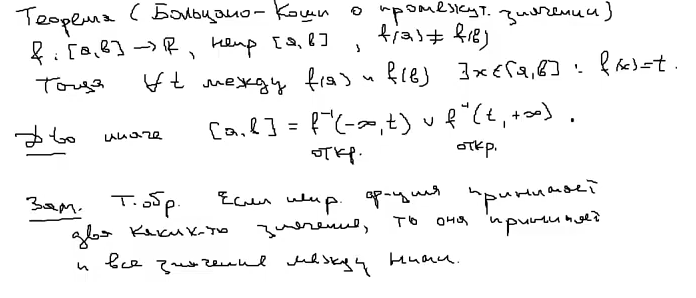
\includegraphics[scale=1.0]{Images/Больцано - Коши.png}





\newpage
\subsection{Теорема о бутерброде}
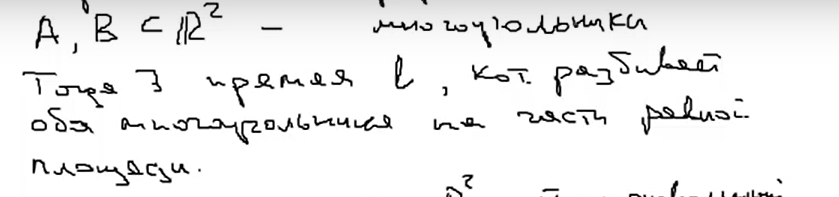
\includegraphics[scale=0.7]{Images/Бутерброд.png}


Доказательство:\\

Лемма: 

$A \subset R^2$, V - произвольный вектор. Тогда $\exists$ прямая с направлением вектора V, делящая фигуру на части одинаковой площади.\\

Доказательство Леммы: \\

Пусть $A \subset [a,b]\times[c,d]$. Не умоляя общности пусть $[a,b] \not \parallel V$. Где $[a,b]$ - часть оси OX.
Рассмотрим координату на оси ОХ 
$\forall t$ $f(t) = S_l (t) - S_r (t)$ 
$f(a) = -S$, а $f(b) = S$.
f - непрерывна: $|f(t_1) - f(t_2)|$ $\leq$ 2 * площадь слоя фигуры между $t_1$ и $t_2$ $\leq$ $2*(d - c)*|t_1 - t_2|$
По теореме Больцано-Коши о промежуточном значении $\exists t_0$ : $f(t_0) = 0$\\


Доказательство Теоремы: \\

$\forall \phi \in [0,2*\pi]$ построим по лемме прямую направленную под углом $\phi$ к оси OX. Она делит A на равновеликие части. $g(\phi) = S^B_l(\phi) - S^B_r(\phi)$. (Площади фигуры B). \\

1 утверждение (очевидное) (для получения периодичности)

$g(\phi + \pi) = -g(\phi)$

2 утверждение (g - непрерывно)

% запиши 1/2 через frac
$g(\phi_1) - g(\phi_2) \leq 4* 1/2 * d^2 * |sin(\phi_1 - \phi_2)|$, где d - диагональ стола.
По теореме Больцано-Коши о промежуточном значении все получается.
% Хотелось бы вывод получше


\newpage
\subsection{Теорема о сохранении промежутка}

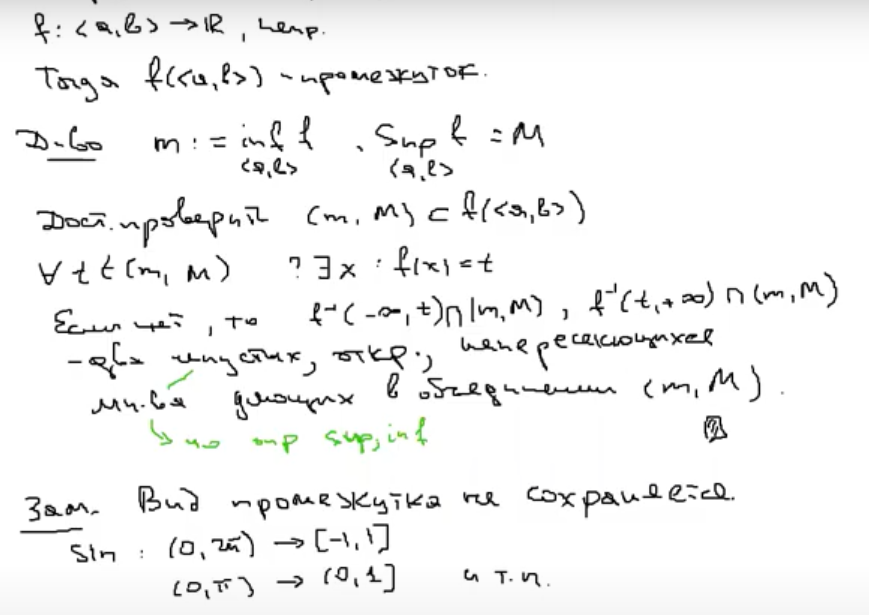
\includegraphics[scale=0.7]{Images/Сохранение промежутка.png}



\newpage
\subsection{Теорема Больцано--Коши о сохранении линейной связности}

Определение: Пусть $Y$ - метрическое пространство и $E \subset Y$.

E - линейно связное если $\forall A,B \in E \  \exists$ путь $c:[a,b] \to E$ - непрерывный, такой что $c(a) = A, c(b) = B$.\\

% непонятно - лучше привести конкретный пример пути
Пример 1 - круг в $\R^2$ - линейно связный потому что выпуклый.\\
$g :[0,1] \to \R^2$\\
$t \to A + t(B - A)$\\

% это не линейно связное мн-во и нужно доказать, почему
Пример 2 - $A \subset \R^2$   
$A = ({0} \times [-1, 1]) \cup \{(x, sin{\frac{1}{x}}) : x \in \R, x \not = 0\}$\\

Теорема :

X - линейное связное множество. $f : X \to Y$ (на Y - сюръекция) - непрерывно.
Тогда Y - линейное связно.\\

Доказательство :

$A, B \in Y$ подберем $U,V \in X$ : $f(U) = A, f(V) = B$;

Соединим U и V путем  с (т.е. возьмем $c : [a, b] \to X, c(a) = U, c(b) = V$). Тогда
% требует пояснения о непрерывности композиции
композиция f и c соединяет точки A и B.

\newpage
\subsection{Описание линейно связных множеств в $\R$}
% зачем тут определение и примеры, когда они есть на предыдущей странице
Определение: Пусть $Y$ - метрическое пространство и $E \subset Y$.

E - линейно связное если $\forall A,B \in E \exists$ путь $c:[a,b] \ to E$ - непрерывный, такой что $c(a) = A, c(b) = B$.\\

Пример 1 - круг в $\R^2$ - линейно связный потому что выпуклый.\\
$g :[0,1] \to \R^2$\\
$t \to A + t(B - A)$\\

Пример 2 - $A \subset \R^2$   $A = ({0} * [-1, 1]) \cup {(x, sin{\frac{1}{2}} : x \in \R, x \not = 0)}$\\

Теорема : 

В $\R^1$ линейно связыми множествами являются только промежутки.\\

Доказательство : 

% оформление не оч
В утверждении спрятана $\leftrightarrow$.
E - промежуток $\rightarrow$ E - линейно связно. Очевидно.
E - линейно связно. $m = \inf E, M = \sup E$. Проверим, что $(m, M)\subset E$.
Пусть $t \in (m, M)$: $t \not \in E$.
% почему такие А и В существуют?
Возьмем $A \in E : A < t$, $B \in E : t < B$

Тогда $\not\exists$ пути из A в B. (Если бы существовал такой путь, 
% почему? поясни
то в некоторой точке $d \in (a,b) : c(d) = t$).


\newpage
\rhead{Хакимов}
\subsection{Теорема о непрерывности монотонной функции. Следствие о множестве точек разрыва}
% а следствие где?
\textbf{Теорема о непрерывности монотонной функции} \\
Пусть $f: \langle a, b \rangle \to \R$, $f$ монотонна. Тогда справедливы следующие утверждения. \\
\begin{enumerate}
    \item $f$ не может иметь разрывов второго рода.
    \item Непрерывность $f$ равносильна тому, что её множество значений - промежуток.
\end{enumerate}
\textit{Доказательство.} Пусть $f$ возрастает(для других случаев доказывается аналогично). \\
\begin{enumerate}
    \item Пусть $x_0 \in (a, b \rangle, x_1 \in \langle a, b)$. Тогда $f(x_1) \leq f(x) \leq f(x_0)$ для всех $x \in (x_1, x_0)$, поэтому 
    % f возрастает не поэтому, а сама по себе - это дано
    %%% я имел ввиду так как f возрастает поэтому...
    $f$ возрастает и ограниченна сверху на $\langle a, x_0)$. По теореме о пределе монотонной функции существует конечный предел $f(x_0-)$, причём по теореме о предельном переходе в неравенстве $f(x_1) \leq f(x_0-) \leq f(x_0)$. Аналогично доказывается, что для любой точки $x_0 \in \langle a, b)$ существует конечный предел $f(x_0+)$, причём $f(x_0) \leq f(x_0+) \leq f(x_2)$ для всех $x_2 \in (x_0, b \rangle$.
    % что-то слишком непонятно закрутил, у Кохася тоже самое изложено более понятным языком
    %%% нуу, я написал что помню, извиняюсь за непонятность
    \item Ввиду следствия, остаётся доказать только достаточность.\\
    Пусть $f(\langle a, b \rangle)$ --- промежуток. Докажем непрерывность $f$ слева в любой точке 
    % зачем выкалывать а?
    $x_0 \in (a, b \rangle$ от противного. Пусть $f(x_0-) < f(x_0)$ (мы уже доказали, что существует конечный левосторонний предел). Возьмём $y \in (f(x_0-), f(x_0))$. Тогда если $a < x_1 < x_0$, то $y \in [f(x_1), f(x_0)]$. Следовательно, $y \in f( \langle a, b \rangle)$, т.е. $y$ - значение функции. С другой стороны $$\forall x \in \langle a, x_0) \Rightarrow f(x) \leq f(x_0-) < y,$$а
    $$\forall x \in [x_0, b\rangle \Rightarrow f(x) \geq f(x_0) > y,$$
    т.е. функция не принимает значение $y$. Получаем противоречие. Т.е. $f(x_0-) = f(x_0)$. Аналогично $f$ непрерывна справа в любой точке $x_0' \in \langle a, b)$.
\end{enumerate}

\subsection{Теорема о существовании и непрерывности обратной функции}
\textbf{Теорема о существовании и непрерывности обратной функции} \\
% забыл условие непрерывности
Пусть $f \in C(\langle a, b \rangle \to \R)$, $f$ строго монотонна, $$m = \inf_{x \in \langle a, b \rangle} f(x),\ \ \ M = \sup_{x \in \langle a, b \rangle} f(x).$$
Тогда справедливы следующие утверждения.\\
\begin{enumerate}
    \item $f$ обратима, $f^{-1}:\langle m, M \rangle \to \langle a, b\rangle$ - биекция.
    \item $f^{-1}$ строго монотонна одноимённо с $f$.
    \item $f^{-1}$ непрерывна.
\end{enumerate}
\textit{Доказательство.} Пусть для определённости $f$ строго возрастает. \\
Если $x_1, x_2 \in \langle a, b \rangle, x_1 < x_2,$ то $f(x_1) < f(x_2)$; следовательно, 
% почему? поясни
$f$ обратима. По теореме о сохранении промежутка $f(\langle a, b \rangle) = \langle m, M\rangle.$ 
% новая теорема?
%%% аййй, забыл что эту теорему я читал из Виноградова:-((
По общим свойствам обратного отображения $f^{-1}$ -- биекция $\langle m, M\rangle\  \text{и}\  \langle a, b\rangle$.\\
Докажем, что $f^{-1}$ строго возрастает. Если $y_1,\ y_2 \in \langle m, M\rangle,\ y_1<y_2,$ то $y_1 = f(x_1),\ y_2 = f(x_2),$ где $x_1,\ x_2 \in \langle a, b\rangle,\ x1 = f^{-1}(y_1),\ x_2 = f^{-1}(y_2)$ При этом $x_1 < x_2$, так как возможность $x_1 \geq x_2$ исключена в силу строгого возрастания $f$.\\
Возрастающая функция $f^{-1}$ задана на промежутке $\langle m, M\rangle$, а её множество значений - промежуток $\langle a, b\rangle$. По теореме о непрерывности монотонной функции она непрерывна.
\subsection{Счетность множества рациональных чисел.}
\textbf{Множество рациональных чисел счётно} \\
\textit{Доказательство.} Обозначим $$Q_+ = \{x \in \Q:  x > 0\}, \ \ \ Q_- = \{x \in \Q\}$$
При всех $q \in \N$ множество $Q_q = \{\frac{1}{q}, \frac{2}{q}, \frac{3}{q},...\}$ счётно. По теореме об объединении не более чем счётных множеств и $Q_+ = \cup_{q=1}^{\infty} Q_q$ счётно. 
% не очевидно и непонятно, опять же можно доказать проще
%%% ну я написал так, как могу/
Очевидно, что $Q_- ~ Q_+$. Снова по той же теореме множество $$\Q = Q_+ \cup Q_-\cup \{0\}$$
счётно.
\subsection{Несчетность отрезка. }
\textbf{Несчетность отрезка} Отрезок $[0, 1]$ несчетен\\
\textit{Доказательство.} Допустим противное: пусть отрезок $[0, 1]$ счетен, т.е. все числа отрезка $[0, 1]$ можно расположить в виде последовательности: $$[0,1] = \{x_1, x_2, x_3, x_4, x_5, ...\}$$
Разобьем отрезок $[0,1]$ на три равных отрезка $[0, \frac{1}{3}],\ [\frac{1}{3}, \frac{2}{3}], [\frac{2}{3}, 1]$ и обозначим через $[a_1, b_1]$ тот из них, который не содержит точки $x_1$(если таких два, то всё равно, какой). Далее разобьём отрезок $[a_1, b_1]$ на три равных отрезка и обозначим через $[a_2, b_2]$ тот из них, который не содержит $x_2$ (если таких более одного, то всё равно, какой). Этот процесс продолжим неограниченно. В результате мы построим последовательность вложенных отрезков $\{[a_n, b_n]\}^{\infty}_{n=1}$, причём $x_n \notin [a_n, b_n]$ для любого $n$. По аксиоме о вложенных отрезках существует точка $x^*$, принадлежащая одновременно всем отрезкам $[a_n, b_n]$. Тем более, $x^* \in [0, 1]$. Но тогда $x^*$ имеет номер: $x^* = x_m$ при некотором $m$. По построению $x^* \notin [a_m, b_m]$, 
% какая-то кривая и неверная фраза
%%% 0_0
что противоречит принадлежности $x^*$ всем отрезкам $[a_n, b_n]$.
\subsection{Континуальность множества бинарных последовательностей}

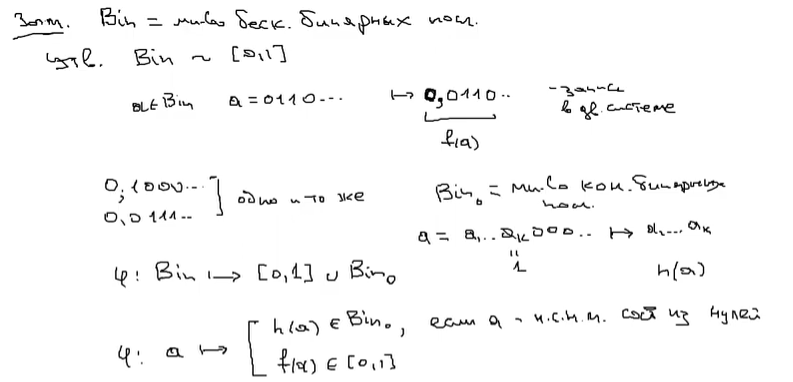
\includegraphics[scale=0.7]{Images/Бин.png}


\newpage
\rhead{Дзестелов}
\subsection{Замечательные пределы}
\textit{Утверждение.} Из геом. соображений верно следующее неравенство $\sin{x} < x < \tan{x}$ для $0 < x < \pi/2$\\

\textbf{Замечательные переделы} \\
\begin{enumerate}
    \item $$\lim_{x \to 0}{\frac{\sin{x}}{x}} = 1$$ \\
    \textit{Доказательство.} Для $0 < x < \pi/2 \quad x < \tan{x} \Rightarrow \cos{x} < \frac{\sin{x}}{x} < 1$, откуда по теореме о двух городовых имеем замечательный предел.
    
    \dotfill
    \item $$\lim_{x \to 0}{\frac{e^x - 1}{x}} = 1$$ \\
    \textit{Доказательство.} (Кохась взял кредит, док-во не требуется)
    
    \dotfill
    \item $$\lim_{x \to 0}{\frac{\ln(1 + x)}{x}} = 1$$ \\
    \textit{Доказательство.} Положим $t = \ln(1 + x) \Rightarrow e^t = 1 + x \Rightarrow x = e^t - 1 \Rightarrow$
    % не совсем, там перевернуть надо
    $$ \lim_{x \to 0}{\frac{\ln(1 + x)}{x}} = \lim_{x \to 0}{\frac{e^t - 1}{t}}
    = 1$$
    Подстановка $t$ справедлива по пределу композиции, т. к. $\ln(1 + x)$ непрерывная функция
    
    \dotfill
    \item $$\lim_{x \to 0}{(1 + x) ^ \frac{1}{x}} = e$$ \\
    \textit{Доказательство.} $(1 + x) ^ \frac{1}{x} = e ^ {\frac{\ln(1 + x)}{x}} \rightarrow e^1 = e$
    
    \dotfill
    % допиши, что верно для любого вещественного альфа
    \item $$\lim_{x \to 0}{\frac{(1 + x)^\alpha - 1}{x}} = \alpha$$ \\
    \textit{Доказательство.} Положим $f(x) = (1 + x)^\alpha - 1 \Rightarrow \ln(f(x)+1) = \alpha\ln(1 + x)$. 
    % необходимо упомянуть, что f(x) -> 0 при x -> 0 и что она удовлетворяет условию существования предела композиции
    Тогда при $x\rightarrow 0$ по двум замечательным пределам: $$\frac{(1+x)^\alpha - 1}{x} = \frac{f(x)}{x} = \frac{f(x)\alpha\ln(1 + x)}{x\ln(f(x) + 1)} = \frac{f(x)}{\ln(f(x) + 1)} \cdot \alpha \cdot \frac{\ln(x + 1)}{x} \rightarrow 1 \cdot \alpha \cdot 1 = \alpha$$
\end{enumerate}

\newpage
\subsection{Равносильность двух определений производной. Правила дифференцирования.}

% вообще-то там отрезки <a, b>
Пусть функция $f$ действует из отрезка $[a, b] \rightarrow \R, x_0 \in (a, b)$.
 
\dotfill
 
\textbf{Определение производной №1} \\ 
% Лучше воткнуть знак умножения между А и (x - x_0), чтобы путаницы не было
Если $\exists A \in \R: f(x) = f(x_0) + A(x - x_0) + o(x - x_0), x \rightarrow x_0$, тогда $f$ - дифф. в $x_0$, а $A$ - производная в этой точке.
 
\dotfill 
 
\textbf{Определение производной №2} \\ 
Если $\exists \lim\limits_{h \to 0} \frac{f(x+h)-f(x)}{h} = A \in \R$, тогда $f$ - дифф. в $x_0$, а $A$ - производная в этой точке. 
 
\dotfill
 
\textbf{Эквивалентность определений} \\
Определение №1 эквивалентно определению №2. \\
 
 % в обратную сторону неочевидно, лучше отдельно в обе стороны расписать по Кохасю
\textit{Доказательство.} $$(1) \Leftrightarrow \frac{f(x) - f(x_0)}{x - x_0} = A + \frac{o(x-x_0)}{x-x_0} \Leftrightarrow 
% скобки можно сделать так, чтобы они подстривались под размер
% лучше расписать этот момент подробнее
(\lim\limits_{x \to x_0} \frac{o(x-x_0)}{x-x_0} = 0) \Leftrightarrow (2)$$
 
\dotfill
 
\textbf{Правила дифференцирования} \\
% опять не тот тип отрезков
Пусть функции $f, g$ действут из отрезка $[a, b] \rightarrow \R, x_0 \in (a, b)$, дифф. в $x_0 \Rightarrow \varphi$ дифф. в $x_0$ и справедливо:
\begin{enumerate}
    \item $\varphi'(x_0) = (f+g)'(x_0)=f'(x_0)+g'(x_0)$
     % ну могу бы и расписать для чайников
    \textit{Доказательство.} По определению.
    
    \item $\forall \alpha \in \R \quad \varphi'(x_0) = (\alpha f(x_0))'= \alpha f'(x_0)$
     
    \textit{Доказательство.} По определению.
     
    \item $\varphi'(x_0) = (fg)'(x_0)=f'(x_0)g(x_0)+f(x_0)g'(x_0)$
    % непонятно, лучше оставить только то, что на картинке
    % хотя и там какие-то непонятные дельты, в отличие от понятного Кохася
    \textit{Доказательство.} \\
     $${{\left( {fg} \right)^\prime } = \lim\limits_{\Delta x \to 0} \frac{{f\Delta g}}{{\Delta x}} + \lim\limits_{\Delta x \to 0} \frac{{g\Delta f}}{{\Delta x}} + \lim\limits_{\Delta x \to 0} \frac{{\Delta f}}{{\Delta x}} \cdot \lim\limits_{\Delta x \to 0} \Delta g } = $$
     $$= {f\lim\limits_{\Delta x \to 0} \frac{{\Delta g}}{{\Delta x}} + g\lim\limits_{\Delta x \to 0} \frac{{\Delta f}}{{\Delta x}} + \lim\limits_{\Delta x \to 0} \frac{{\Delta f}}{{\Delta x}} \cdot \lim\limits_{\Delta x \to 0} \Delta g } = {fg' + gf' + f' \cdot 0 } = {f'g + fg'.}$$
      
    (optional) \\
    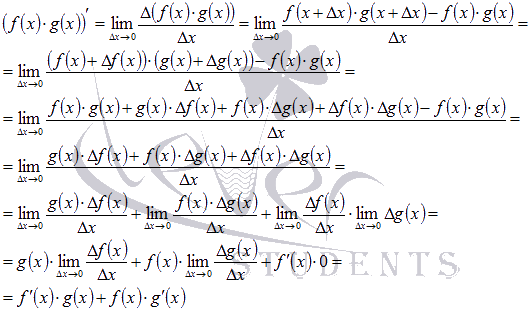
\includegraphics[scale=0.5]{Images/производная произведения.png}
      
    \dotfill
    
    \item $g(x_0) \not=0 \Rightarrow\varphi'(x_0) = (\frac{f}{g})'(x_0)=\frac{ f'(x_0)g(x_0)-f(x_0)g'(x_0)}{g^2(x_0)}$
    
    \textit{Доказательство.}  
    % опять непонятно, что за \delta f(x)
    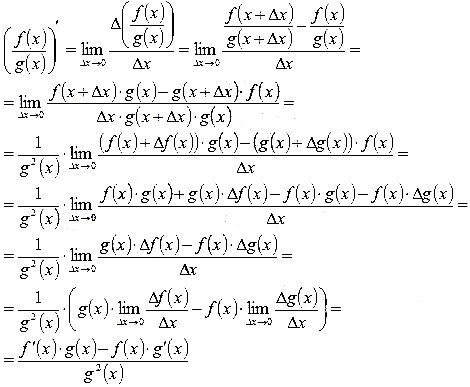
\includegraphics[scale=1]{Images/производная частного.jpg}
\end{enumerate}

\newpage
\subsection{Дифференцирование композиции и обратной функции}
    
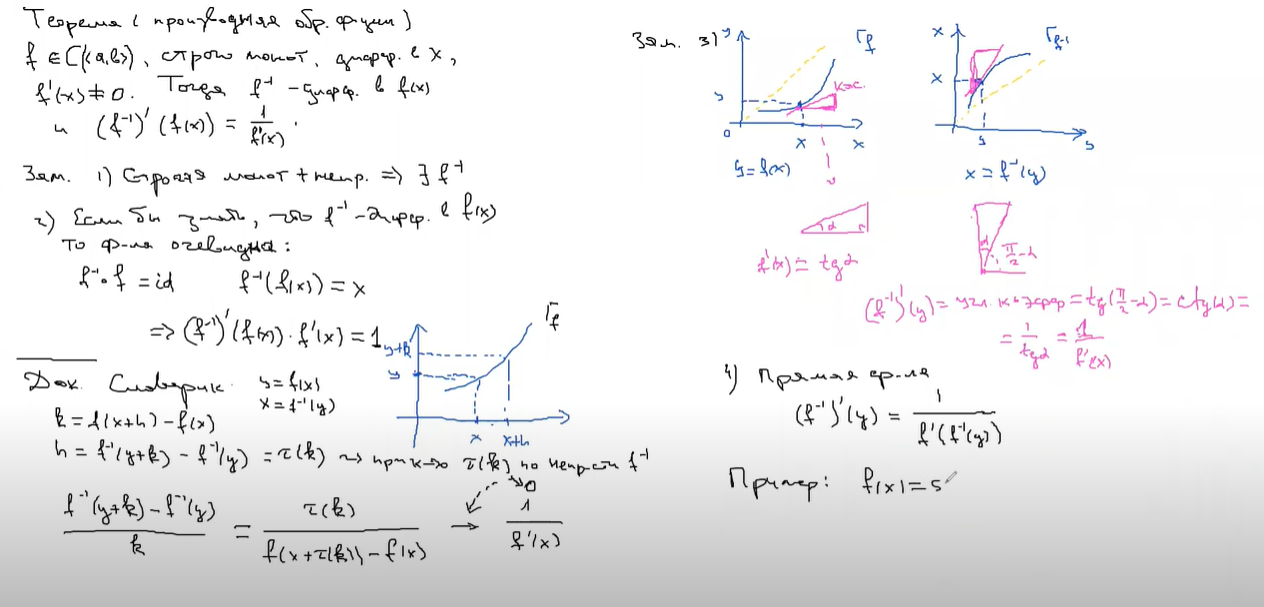
\includegraphics[scale=0.5]{Images/Обратная.png}

\newpage
\subsection{Теорема о свойствах показательной функции}

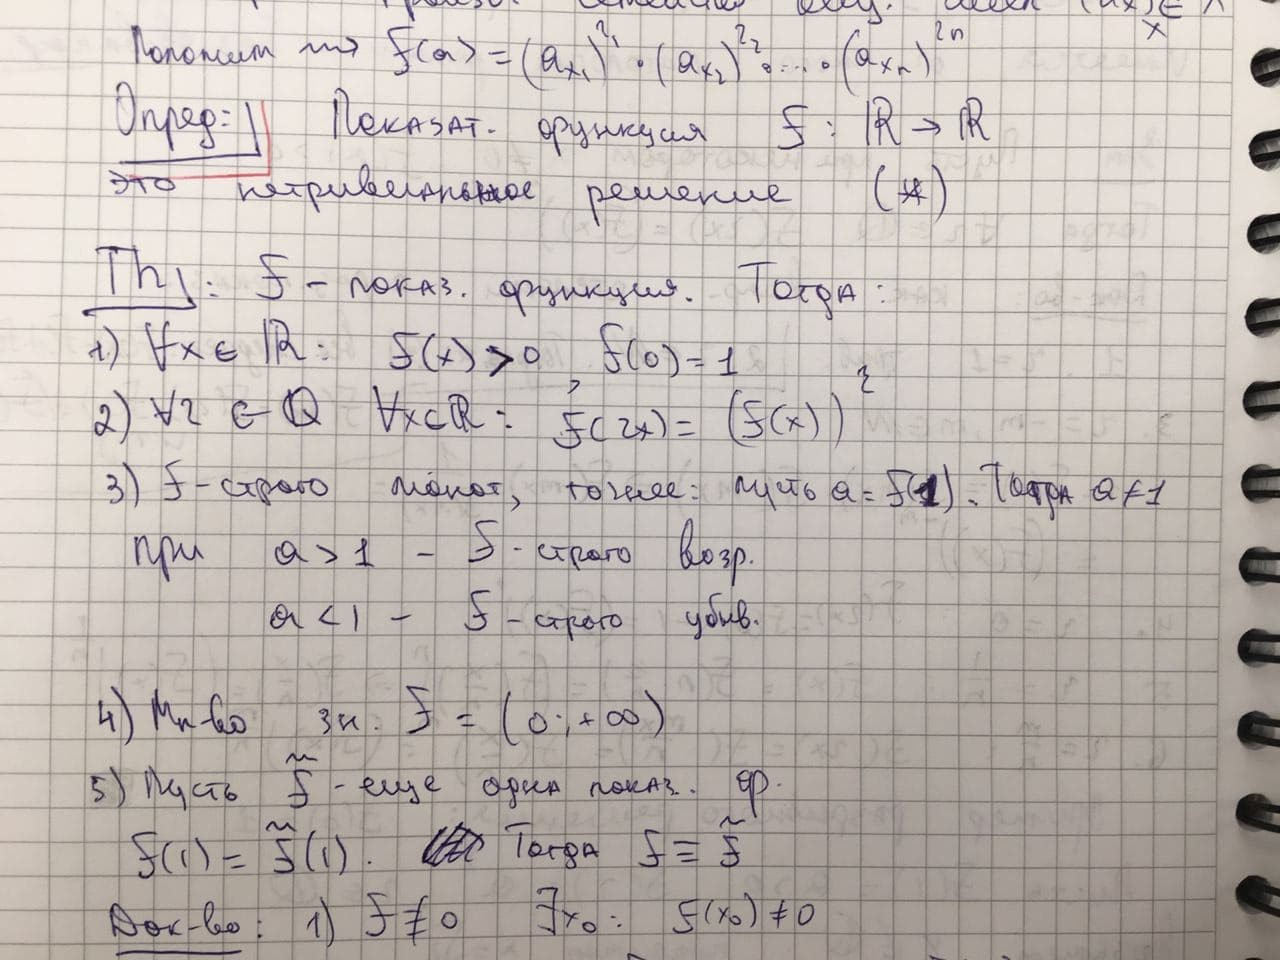
\includegraphics[scale=0.5]{Images/photo_2021-01-26_09-51-22.jpg}

\newpage
\subsection{Выражение произвольной показательной функции через экспоненту. Два следствия}

\newpage
\rhead{???}
\subsection{Показательная функция от произведения}

\newpage
\rhead{Алексеев}
\subsection{Теорема Ферма (с леммой)}

\newpage
\rhead{Галибов}
\subsection{Теорема Ролля. Вещественность корней многочлена Лежандра}

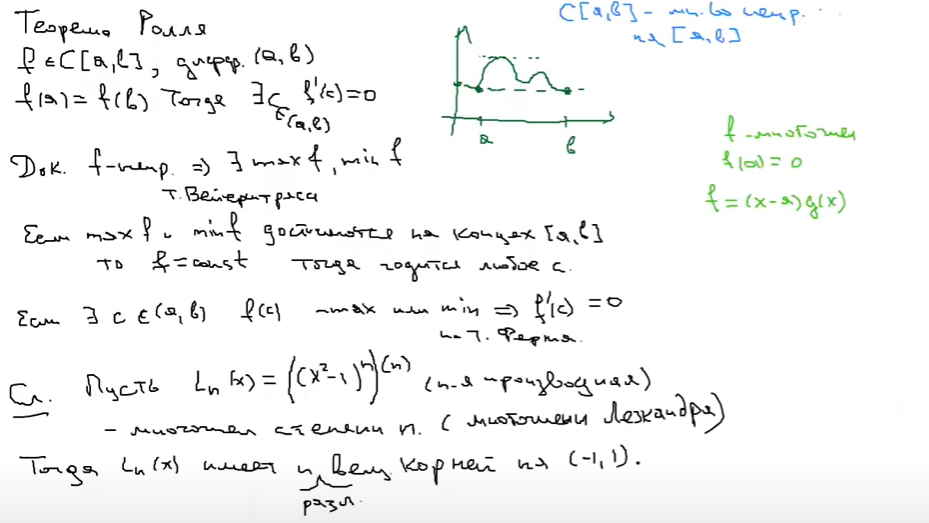
\includegraphics[scale=0.7]{Images/ролль.png}

\newpage
\rhead{Хакимов}
\subsection{Теоремы Лагранжа и Коши. Следствия об оценке приращения и о пределе производной}
\textbf{Теорема Лагранжа.} Пусть функция $f$ непрерывна на $[a, b]$ и дифференцируема на $(a, b)$. Тогда найдётся такая точка $c \in (a, b)$, что $$\frac{f(b)-f(a)}{b-a} = f'(c).$$ \\
\textbf{Теорема Коши.} Пусть функции $f$ и $g$ непрерывны на $[a, b]$ и дифференцируемы на $(a, b)$, $g'(x) \neq 0$ для любого $x \in (a, b)$. Тогда найдётся такая точка $c \in (a, b)$, что $$\frac{f(b)-f(a)}{g(b)-g(a)} = \frac{f'(c)}{g'(c)}.$$ \\
\textbf{Замечание.} Теорема Лагранжа - частный случай теоремы Коши, где $g(x) = x$. Поэтому достаточно доказать теорему Коши. \\ \\
\textit{Доказательство} теоремы Коши. Заметим, что $g(a) \neq g(b)$, так как инчае по теореме Ролля нашлась бы точка $t \in (a, b)$, в которой $g'(t) = 0$. Положим $h = f-Kg$, где $K = \frac{f(b)-f(a)}{g(b)-g(a)}$, т.е. $h(a) = h(b)$. Тогда $h$ удовлетворяет условиям теоремы Ролля. Поэтому найдётся такая точка $c \in (a, b)$, что $h'(c) = 0$, т.е. $f'(c) = Kg'(c)$. 
% распиши лучше - непонятно, к чему мы пришли
Что и требовалось доказать.
\\
\\
% мб докажешь следствие? и есть ещё одно следствие
\textbf{Следствие. Оценка приращения функции.} Пусть функция $f$ непрерывна на 
% у Кохася замкнутый отрезок
$\langle a, b \rangle$, дифференцируема на $(a, b)$, а число $M > 0$ таково, что $|f'(t)| \leq M$ для всех $t \in (a, b)$. Тогда для любых точек $x$ и $x+\Delta x$ из $\langle a, b \rangle$ $$|f(x+\Delta x)-f(x)|\leq M|\Delta x|.$$
\newpage
\rhead{Дзестелов}
\subsection{Теорема Дарбу. Следствия}

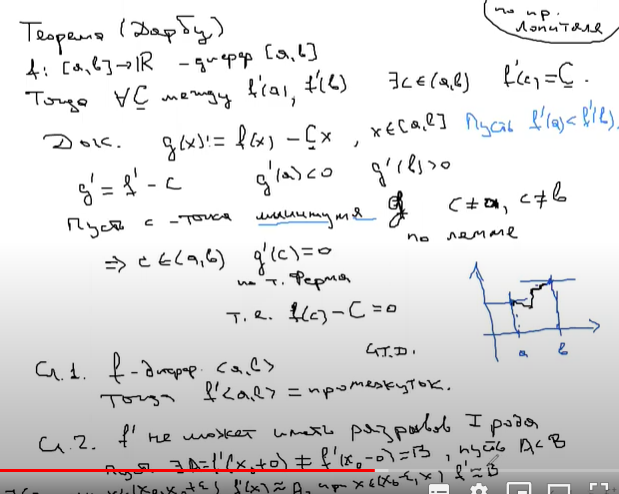
\includegraphics[scale=1.0]{Images/Дарбу.png}

\newpage
\rhead{Шехунов}
\subsection{Формула Тейлора с остатком в форме Пеано}
\textit{Пусть в точке $x_0$ функция $f(x)$ имеет производную n-го порядка, $P_n(x)$ - её многочлен Тейлора степени $n$ в точке $x_0$ ($n \geq 1$). $\mathbf{f(x) = P_n(x) + o(x - x_0)^{n}}$, при $x \rightarrow x_0$} \\
\textbf{Доказательство.} \\
Напомним \textbf{основное свойство многочлена Тейлора}: \textit{Функция $f(x)$ и её многочлен Тейлора $P(x)$ степени $n$ в точке $x_0$, а так же все их производные до n-го порядка включительно имеют равные значения.} \\
Обозначим $R(x) = f(x) - P_n(x)$ 
% какого нахуй св-ва?! расписать нормально не судьба?
Из основного свойства многочлена Тейлора следует \\
$R(x_0) = R'(x_0) = R''(x_0) = \dots = R^{(n)}(x_0) = 0$ \\
Из непрерывности в точке $x_0$ функций $R(x), R'(x), \dots, R^{(n-1)}(x)$ следует, что: 
$$\lim_{x \to x_0} R(x) = \lim_{x \to x_0} R'(x) = \dots = \lim_{x \to x_0} R^{(n-1)}(x) = 0$$
Нам надо доказать, что 
% степень где?
$R(x) = o(x-x_0)$ при $x \rightarrow x_0 \Longleftrightarrow \mathbf{\lim_{x \to x_0} \frac{R(x)}{(x-x_0)^{n}} = 0}$ \\
Применим $n-1$ раз правило Лопиталя: 
$$\lim_{x \to x_0} \frac{R(x)}{(x-x_0)^n} = \left[ {0\over0} \right] = \lim_{x \to x_0} \frac{R'(x)}{n(x-x_0)^{n-1}} = \left[ {0\over0} \right] = \lim_{x \to x_0} \frac{R''(x)}{n(n-1)(x-x_0)^{n-2}} = \left[ {0\over0} \right] =$$
$$= \dots = \lim_{x \to x_0} \frac{R^{(n-1)}(x)}{n\cdot(n-1)\cdot \dots \cdot 2 \cdot (x-x_0)} = \frac{1}{n!} \lim_{x \to x_0} \frac{R^{(n-1)}(x) - R^{(n-1)}(x_0)}{(x-x_0)} = $$
$$=\frac{1}{n!}(R^{(n-1)}(x_0))' = \frac{1}{n!}R^{(n)}(x_0) = 0$$
На последнем этапе мы получили по определению производную функции $R^{(n-1)}(x)$ в точке $x_0$. \qedsymbol
\newpage
\rhead{Альжанов}
\subsection{Теорема о разложении рациональной функции на простейшие дроби}$ $\\
\begin{theorem}
$f(x) = \frac{P(x)}{Q(x)}$ несократимая дробь, P, Q {---} многочлены, такие что степень многочлена $P$ $<$ степени многочлена $Q$, ($deg\ P < deg\ Q$)


Q(x) разлагается на множители.

$Q(x) = (x-\alpha_1)^{k_1} \cdot (x-\alpha_2)^{k_2} \cdot \dots \cdot (x-\alpha_m)^{k_m} $, $\alpha$ - вещественные


Тогда $\exists A_1, \dots A_{k_1};\ B_1, \dots B_{k_2};\ \dots;\ D_1, \dots D_{k_m} \in $, где $A, B, \dots, D$ --- для каждого корня соответственно, такие что:

$$\frac{P(x)}{Q(X)} = (\frac{A_1}{x-\alpha_1} + \frac{A_2}{(x-\alpha_1)^2} + \dots + \frac{A_{k_1}}{(x-\alpha_1)^{k_1}}) +$$
$$(\frac{B_1}{x-\alpha_1} + \dots + \frac{B_{k_2}}{(x-\alpha_1)^{k_1}}) + \dots +  (\frac{D_1}{x-\alpha_1} + \dots + \frac{D_{k_m}}{(x-\alpha_1)^{k_1}})\ \ (\star)$$
\end{theorem}
\begin{proof}
Для $\alpha_1$:

$\displaystyle Q(1)=(x-\alpha_2)^{k_2}\dots(x-\alpha_m)^{k_m}$

$\displaystyle\frac{P}{Q}=\frac{1}{(x-\alpha)^{k_1}}\cdot\frac{P}{Q_1}$

$\displaystyle Q_1^{(\alpha_1)} \neq 0 \Rightarrow \frac{P}{Q_1}$ {---} бесконечно дифферинциируема в окрестности точки $\alpha_1$ (из опыта дифференциируемости) 

Воспользуется формулой Тейлора:

$x_0=\alpha_1$

$\displaystyle \frac{P}{Q_1} = A_{k_1} + A_{k_{1} - 1}\cdot(x - \alpha_1) + \dots + A_1(k-\alpha_1)^{k_1 - 1} + A_0(k-\alpha_1)^{k_1} + o((x-\alpha_1)^{k_1})$, $x \to \alpha_1$`
 
$\displaystyle \frac{P}{Q} = \frac{A_{k-1}}{(x-\alpha_1)^{k_1}} + \dots + \frac{A_1}{x-\alpha_1}+A_0+o(1)$, $x\to\alpha_1$

Аналогично получаем $B, \dots D$

Проверим, что равно предположению:

$$\frac{P}{Q} - (\star) = (\frac{P}{Q} - (\frac{A_{k_1}}{(x-\alpha_1)^{k_1}} + \dots + \frac{A_1}{x-\alpha_1})) - (\frac{B_1}{x-\alpha_1} + \dots) - \dots$$ 

Из этой разности при "упрощении выражения" сокращаются все множители знаменателя, значит останется многочлен (или константа)

$\displaystyle\frac{P}{Q} - (\star) \xrightarrow[x\to \infty]{} 0 \Rightarrow$ это $ \equiv 0$


\end{proof}
\newpage
\subsection{Формула Тейлора с остатком в форме Лагранжа}
\begin{theorem*}
$f \in C^n (a; b)$ - дифф. $n$ раз на отрезке $(a; b)$;
$(n+1)$ раз дифф. на (a; b);
$x_\alpha,\ x_0 \in (a; b)$


Тогда $\exists c \in (x_0, x)$
$$f(x) = \sum^{n}_{k=0} \frac{f^{(k)}(x_0)}{k!}(x-x_0)^k+\frac{f^{(n+1)}(c)}{(n+1)!}(x-x_0)^{n+1}$$
\end{theorem*}
\begin{proof}
$$
\varphi(t) := f(x)-\sum_{k=0}^{n} \frac{f^{(k)}(t)}{k !}(x-t)^{k}
$$
$$
\varphi'(t)=-f^{\prime}(t)-\sum_{k=1}^{n} \frac{f^{(k+1)}(t)}{k !}(x-t)^{k}-\frac{f^{(k)}(t)}{(k-1) !}(x-t)^{k-1}
$$
$$
=-f'(t)-\left(-f^{\prime}(t)+\frac{f^{(n+1)}(t)}{n !}(x-t)^{n}\right)=-\frac{f^{(n+1)}(t)}{n !}(x-t)^{n}
$$
$$
\varphi(x_{0})=f(x)-T_{n}(f, x_{0})(x)=R_{n}(f, x_{0})(x)
$$
$$
\psi(t) := (x-t)^{n+1}
$$

По Т. Коши: $\exists c: $

$$
\frac{-R_{n}}{-\left(x-k_{0}\right)^{n+1}} = \frac{\varphi(x)-\varphi\left(x_{0}\right)}{\psi(x)-\psi\left(x_{0}\right)} = \frac{\varphi^{\prime}(c)}{\psi^{\prime}(c)}=\frac{-\frac{f^{(n+1)}(c)}{n !}}{-(n+1)(x-c)^n}
$$

$$
R_n = \frac{f^{(n+1)}(c)}{(n+1)!}(x-x_0)^{n+1}
$$

\end{proof}
\subsection{Метод Ньютона}$ $\\
Находит приблежённое решение уравнения

Так же называют метод Касательных.

Берём "хорошее" начало прибл. $x_1$. Какое для нас будет хорошее - выяним потом.

$x_{n+1} = x_n - \frac{f(x_n)}{f'(x_n)}$

Оценим скорость сходимости.

Пусть $\xi$ {---} это корень

$\displaystyle \xi - x_{n+1} = \xi - x_n + \frac{f(x_n)}{f'(x_n)} = \frac{f(x_n)+ f'(x_n)(\xi-x_n)}{f'(x_n)} \textcircled{=}$ - в числителе кусок формулы тейлора. Напомним:
$\displaystyle f(\xi) = f(x_n)+ f'(x_n)(\xi-x_n) + \frac{1}{2} f''(c)(\xi-x_n)^2$, $c$ - межуд $x_n$ и $\xi$

$\textcircled{=} -\frac{1}{2} \frac{f''(c)}{f'(x_n)}(\xi-x_n)^2$

Пусть $\max\abs{f''} = M$, а $\min\abs{f'} = m > 0$,

Теперь мы можем сказать, что

$\displaystyle
\abs{\xi-x_n+1} \leqslant 
\frac{M}{2m}-\abs{\xi - x_n}^2 \leqslant
\frac{M}{2m}\cdot(\frac{M}{2m}\abs{\xi-x_{n-1}}^2)^2\leqslant
(\frac{M}{2m})^{1+2}\cdot(\frac{M}{2m}\abs{\xi-x_{n-2}}^2)^2\leqslant
\dots\leqslant
(\frac{M}{2m})^{1+2+4+\dots+2^{n-1}}\cdot\abs{\xi\cdot x_1}^{2^n} =
\frac{2m}{M} \cdot (\frac{M}{2m} \abs{\xi - x_1})^{2^{n}}
$


Теперь можем составить "хорошее" определение для $x1$: 

$\displaystyle \frac{M}{2m}\abs{\xi-x1} < 1$
\subsection{Иррациональность числа $e^2$}
\begin{theorem*}
$e^2$ - иррационально
\end{theorem*}
\begin{proof}
От противного.


Пусть $e=\frac{2k}{n}$ (м.б. n - чётно)

$$e n = 2k \cdot e^{-1} \Rightarrow e n \cdot (2k-1)!=(2k)!e^{-1}$$

$e^1=1+1+\frac{1}{2!} + \dots + \frac{1}{(2k-1)!} + \frac{e^c}{(2k)!}$ - по формуле Тейлора. $x_0 = 0, x = 1, 0 < c < 1$

Левая часть:
$\displaystyle e(2k-1)!=\underbrace{n(2k-1)!(1+1+\frac{1}{2!}+\dots+\frac{1}{(2k-1)!})}_\textrm{Целое число} + \underbrace{\frac{n}{2k}\cdot e^c}_{\frac{e^c}{e^2} = e^{c-2} < \frac{1}{e}}$

Получаем, что левая часть чуть больше целого числа.

Так же распишем $e^{-1}$ используя ф. Тейлора $x_0 = 0, x=-1, -1 < c_1 < 0$

$\displaystyle e^{-1} =  1-1+\frac{1}{2!}-\frac{1}{3!}+\dots+\frac{1}{(2k)!}-\frac{e^{c_1}}{(2k+1)!}$

Правая часть:
$\displaystyle \underbrace{(2k)!\left(1-1+\frac{1}{2!}-\frac{1}{3!}+\dots+\frac{1}{(2k)!}\right)}_\textrm{Целое число}-\underbrace{(2k)!\cdot\frac{e^{c_1}}{(2k+1)!}}_{\frac{e^{c_1}}{2k+1}<\frac{1}{3}}$

Получилось, что правая часть чуть меньше целого

Получили противоречие, следовательно $e^2$ - иррационально
\end{proof}
\subsection{Следствие об оценке сходимости многочленов Тейлора к функции. Примеры}
F
\subsection{Критерий монотонности функции. Следствия}
\begin{theorem*}

\end{theorem*}
\subsection{Теорема о необходимом и достаточном условиях экстремума}
\subsection{Теорема Кантора о равномерной непрерывности}

\newpage
\section{Определения и формулировки}
\setcounter{subsection}{2}

\rhead{Шемякин}
\subsection{Упорядоченная пара}
Упорядоченная пара {—--} двухэлементное семейство, где множеством индексов является \{1,2\}.

Множество {---} набор различных элементов. Неопределяемое понятие.

Семейство {---} мультимножество, индексированное элементами другого множества

\newpage
\subsection{Декартово произведение}
Декартовым или прямым произведением множеств $X$ и $Y$ называется множество всех упорядоченных пар, таких, что первый элемент пары принадлежит $X$, а второй — $Y$:
$X \times Y = \{(x,y):x \in X,y\in Y\}$

\newpage
\subsection{Аксиомы вещественных чисел}
\subsubsection*{\RomanNum 1 Аксиомы Поля}
Множество $R$ действительных чисел, в котором введены операции $+$ и $*$ и отношения порядка, если выполняются следующие аксиомы
        \\ $ +\;1.$ \ Коммутативность $ \forall a,b \in R : a + b = b + a $
		\\ $ +\;2. $ \ Ассоциативность $ (a+b)+c = a + (b + c) $
		\\ $ +\;3. $ \ Существование нейтрального элемента по сложению: $ \exists \0 : \forall a : a + \0 = a $
		\\ $ +\;4. $ \ Существование обратного элемента по сложению: $ \forall a \ \exists  (-a) : a + (-a) = 0 $
		\\
		\\ $ \cdot \; 1. $ \ Коммутативность $ a \cdot b = b\cdot a $
		\\ $ \cdot \; 2. $ \ Ассоциативность $ a\cdot (b \cdot c) = (a \cdot b) \cdot c $
		\\ $ \cdot \; 3. $ \ Существование нейтрального элемента по умножению: $ \exists \1 \neq 0 : \forall a \ \ a \cdot \1 = a $
		\\ $ \cdot \; 4. $ \ Существование обратного элемента по умножению: $ \forall x \neq 0 \ \ \exists  x^{-1} : \ x \cdot x^{-1} = 1  $
		\\
		\\ $ +\cdot \; 1. $ Дистрибутивность $ a \cdot (b+c) = (a\cdot b) + (a\cdot c) $
		\\
		\begin{remark}
		    Нетривиальность поля $1 \neq 0$
		\end{remark}
		\begin{definition}
		    \textbf{Поле} --- множество в котором введены операции "+" и "$\cdot$" удовлетворяющие \RomanNum{1} группе аксиом. Например, $\R, \Q$
	    \end{definition}
	\subsubsection*{\RomanNum 2 Аксиомы порядка}
	
  	\begin{remark}
  		На элементах должно быть введено отношение порядка : $ a \in x, b \in x \ \ a \prec b, \ \prec  \text{--- неравенство} $
  	\end{remark}
   	
  	\begin{enumerate}
  	% с какого блять перепугу это рефлексивность?!
	  \item Рефлексивность: $ \forall x,y \in \R : x \le y \text{ или } y \le x $
	  \item Транзитивность: $ x \le y, y \le z \Rightarrow x \le z $
	  % с хуя ли это антисимметричность?! что ты несешь?!
	  \item Антисимметричность: $ x \le y, y \le x \Rightarrow x = y $
	  % подпиши, что для любого z
	  \item Связь сложения и порядка $ x \le y \Rightarrow x + z \le y + z $
	  \item Связь умножения и порядка $ 0 \le x, ~ 0 \le y \Rightarrow 0 \le xy $
	\end{enumerate}
	\begin{definition}
		Поле, удовлетворяющие аксиомам \RomanNum 1 - \RomanNum 2 называется \textbf{упорядоченным полем}. Например, $\R, \Q$ --- упорядоченное поле, $\C $ --- нет. 
	\end{definition}
	
	\begin{exercise}
		Докажите что $ 0 < 1 $, используя аксиомы  \RomanNum 1 - \RomanNum 2
		
		(Если спросит - гугли. Есть в зориче, лучше прочитать заранее. \textit{Добавил док-во.})
		
		Докажем, что $(-1) * (-1) = 1$. $(-1) * (-1) + (-1) = (-1) * (-1) + (-1) * 1 = (-1) * ((-1) + 1) = (-1) * 0 = 0$. Так как обратный элемент по сложению единственен, то $(-1)*(-1) = 1$. Теперь предположим, что $1 \leq 0$. Тогда $1 \leq 0 \Rightarrow 0 \leq -1$. Но так как $0 \leq -1$ и $0 \leq -1$, то $0 \leq (-1) * (-1) = 1$, противоречие. Значит $0 \leq 1$. Так как по аксиоме $1 \neq 0$, то $0 < 1$. 
	\end{exercise}
   	
  	\begin{remark}
  		 $$ [a,b] = \{ x \in \R: a \le x \le b \} $$
  		 $$ (a,b) = \{ x \in \R: a < x < b \} $$
  		 $$[a,b) = \{ x \in \R: a \le x < b \} $$
  		 $$ (a,b] = \{ x \in \R: a < x \le b \} $$
  		 \textbf{Луч:} $ [a, + \infty) = \{ x : a \le x \} $
  	\end{remark}
   	
  	Аксиома Архимеда и Полноты читать далее.
   	
  	\nobreakspace 
   	
   	 

\newpage
\subsection{Аксиома Кантора, аксиома Архимеда}
	\subsubsection*{\RomanNum 3 Аксиома Архимеда}
  	$ \forall x,y \in \R ~x > 0, y > 0 ~ \exists n \in \N \quad nx > y$
   	   	
  	\begin{consequence}
  		Существуют сколько угодно большие числа
  	\end{consequence}
    
  	\begin{example}
  	% нормальный блять, просто его надо прямыми руками написать
  	    Здесь был пример но он такой хуевый что мы его закоментили. Оставь надежду всяк его читающий.
  		%  $$ R(x) = \big\{ \frac{p(x)}{q(x)}, ~ p, q - \text{многочлены с вещественными коэфициентами} \} $$
  		% \\ $$ \frac{p1}{q1} = \frac{p2}{q2},  \text{ если } \exists ~ T > 0 ~ \forall x > T \ \frac{p_1(x)}{q_1(x)} = \frac{p_2(x)}{q_2(x)} $$
  		% \\  $$ \frac{p1}{q1} < \frac{p2}{q2},  \text{ если } \exists ~ T > 0 ~ \forall x > T \ \frac{p_1(x)}{q_1(x)} < \frac{p_2(x)}{q_2(x)} $$
   	
  	\end{example}
   	
  	\subsubsection*{Аксиома Кантора}
   	
  	Пусть у нас есть последовательность вложенных отрезков $ [a_1,b_1] \supset [a_2, b_2] \supset [a_3, b_3] \ldots $ Тогда для любой бесконечной последовательности вложенных отрезков их пересечение не пусто:
  	$ \bigcap\limits_{k = 1}^{\infty} [a_k, b_k] \neq \varnothing $ 	

	\begin{remark}
	Аксиома Кантора не выполняется для последовательности вложенных промежутков.
	$ \bigcap\limits_{k = 1}^{\infty} (a_k, b_k) = \varnothing $ 	
	
	Например, $(a_k, b_k) = (0, \frac{1}{k}).$ Тогда $\bigcap\limits_{k=1}^{\infty} = \varnothing $
		\begin{proof}
			От противного. Пусть существует $\alpha > 0 (\alpha \le 0$ очевидно, не подходит), что $ \alpha \in \bigcap\limits_{n=1}^{\infty} \left(0, \frac{1}{k}  \right)$ %k=1
			$$\forall k : \alpha < \frac{1}{k}$$ 
			$$\forall k: ak < 1$$ --- Противоречие аксиоме Архимеда
		\end{proof}	
	\end{remark}

\newpage
\subsection{Пополненное множество вещественных чисел, операции и порядок в нем}
% что тут делают операции над множествами? у тебя пункт иначе назывется
Операции над множествами

Пусть $ { ( {x_{n}} )_{\alpha \in A }}$— семейство множеств. Объединением семейства $ { ( {x_{n}} )_{\alpha \in A }}$ называется множество всех элементов, которые принадлежат хотя бы одному из множеств $X_\alpha$:

$\bigcup\limits_{\alpha \in A} X_\alpha = \{ x: \exists \alpha \in A \ \ \ x \in X_\alpha \}$

Пусть $ { ( {x_{n}} )_{\alpha \in A }}$ — семейство множеств. Пересечением семейства $ { ( {x_{n}} )_{\alpha \in A }}$ называется множество всех элементов, которые принадлежат каждому из множеств $X_\alpha$:

$\bigcap\limits_{\alpha \in A} X_\alpha = \{ x: \forall \alpha \in A \ \ \ x \in X_\alpha \}$

Разностью множеств $X$ и $Y$ называется множество всех элементов, которые принадлежат $X$, но не принадлежат $Y$:

$X \setminus Y = \{ x: x \in X, x \notin Y\}$


Дополнение множества: $ \bar A = A^c = \{ x \in \U: x \notin A \}  , \quad \U  \text{ ---универсум}$ 

$ A \setminus B = A \cap B^c  $

% выдели его как-то, а то сливается
Пополненное множество вещественных чисел, операции и порядок в нем

Множество $\bar R = R\bigcup\{-\infty,\infty\}$ называется расширенной числовой прямой.
% опять откуда это в данном пункте
Множество $E \subset R$ называется ограниченным сверху, если существует такое число $M\in R$, что $x \leqslant M$ для всех $x \in E$. Число M называется верхней границей множества.

Множество $E \subset R$ называется ограниченным снизу, если существует такое число $m\in R$, что $x \geqslant m$ для всех $x \in E$. Число m называется нижней границей множества.

Множество $E \subset R$ называется ограниченным, если оно ограничено и сверху, и снизу.

Пусть $ \overline{\R} \textbf{ --- расширенное множество} \text{ вещественных чисел.} $
  	   $ \overline \R = \R \cup \{ + \infty, - \infty \} $ --- не поле, так как некоторые операции не определены
   	   
  	\begin{minipage}{0\textwidth}
	  \begin{flushleft}
		\begin{tabular}{|c|c|c|c|} \hline
  	    $+$ & $x \in \R$ & $+ \infty$ & $- \infty$ \\ \hline 
  		$y \in \R $ & $x+y$ & $+ \infty$ & $- \infty$  \\ \hline 
        $+ \infty $ & $+ \infty$ & $+ \infty$ &  \frownie{} \\ \hline 
        $- \infty $ & $- \infty $ & \frownie{} & $- \infty$  \\ \hline 
  \end{tabular} 
	  \end{flushleft}
	\end{minipage} 
	\begin{minipage}{0.7\textwidth}
	  \begin{flushright}
		\begin{tabular}{|c|c|c|c|c|} \hline
	   	    $\cdot$ & $x > 0$ & 0 & $+ \infty$ & $- \infty$ \\ \hline 
	   		$y < 0 $ & $xy$ & 0 & $- \infty$ & $+ \infty$  \\ \hline 
	        $+ \infty $ & $+ \infty$ & \smiley{} & $+ \infty$ &  $- \infty$ \\ \hline 
	        $- \infty $ & $- \infty$ & \smiley{} & $-\infty$ & $+\infty$  \\ \hline 
	   \end{tabular} 
	  \end{flushright}
	\end{minipage}
   	 
  	\begin{remark} \nobreakspace \\
  		\frownie{} --- не определено \\
  		\smiley{} --- тоже не определено, но уже чуть лучше потому, что в некоторых случаях можно доопределить (например площадь прямоугольника со сторонами $\infty$ и $0$ очевидно равна 0)
  	\end{remark}

$\frac{0}{0} =$ неопределенность

$\frac{\infty}{\infty} =$ неопределенность

$0 * \infty =$ неопределенность

$\infty - \infty =$ неопределенность

$1^\infty =$ неопределенность

$0^0 =$ неопределенность

$\infty^0 =$ неопределенность

$-\infty < \infty$

$\infty * \infty = \infty$

$-\infty * \infty = -\infty$

$-\infty * -\infty = \infty$

$-\infty < X < \infty$

$x + x = 2x$

$x + \infty = \infty$

$x - \infty = - \infty$

$\infty + \infty = \infty$

$-\infty - \infty = -\infty$

$x * x = x^2$
% если х больше нуля

$x * \infty = \infty$
% только если х больше нуля

$x * (-\infty) = -\infty$
\newpage

\rhead{Зайцев}
% не помешало бы ещё определение через семейство - оно понятнее
\subsection{Последовательность}
\textbf{Последовательность} - частный случай отображения\\
$\mathbb{N} \rightarrow Y$\\
По натуральному номеру генерируем точку в пространстве\\
$n \mapsto x_n$\\
Числу $n$ ставим в соответствие элемент из $Y$ который называем $x_n$.\\
\newline
\noindent При желании можно считать последовательность функцией\\
Если выписать множество значений последовательности ($x_1, x_2, x_3...$),\\
то можно воспринимать ее как список.\\
\newline
% да вроде определяемое
% Первая минута третьей лекции, Кохась сказал, что неопределяемое
\textbf{Отображение} - Неопределяемое понятие.\\
Это тройка ($X, Y, f$): \\
$X$ - область опредления\\
$Y$ - множество на котором отображение принимает значения\\
$f$ - правило которое по элементам множества $X$ генерирует элементы множества $Y$\\
$f: X \rightarrow Y$\\
$x \mapsto f(x)$\\
\newline
\textbf{Частные случаи отображения:}
\begin{itemize}
\item Последовательность
\item Функция:\\
$f: X \rightarrow \mathbb{R}$
\item Семейство:\\
$A$ - множество меток\\
$X$ - множество обьектов\\
По каждой метке $\alpha$ из $A$ генерируем $x_\alpha$\\
$\{ x_\alpha \}_{\alpha \in A}$
\end{itemize}

\newpage
\subsection{Образ и прообраз множества при отображении}
Пусть дано отображение $f: X \rightarrow Y$, тогда образом множества $A \subset X$ под действием $f$ называется\\
$f(A) = \{f(x) \ |\ x \in A\}$\\
Прообразом множества $B \subset Y$ относительно отображения $f$ называется\\
$f^{-1}(B) = \{x \in X \ |\ f(x) \in B\}$

\newpage
\subsection{Инъекция, сюръекция, биекция}
Отображение $f$ называется:
\begin{itemize}
\item Сюръекцией (отображением на):\\
$\forall y \in Y \ \exists x \in X: f(x) = y$\\
$\Leftrightarrow f(X) = Y$\\
$\Leftrightarrow \forall y \in Y$ уравнение относительно $x$, $f(x) = y$ - имеет решение
\item Инъекцией (отображением в):\\%взаимооднозначные
$\forall x_1 \in X \ \forall x_2 \neq x_1 \ f(x_1) \neq f(x_2)$\\
$\Leftrightarrow \forall y \in Y$ уравнение $f(x) = y$ имеет не более одного решения (относительно $x$)
\item Биекцией:\\
Если обладает свойствами инъективности и сюръективности\\
$\Leftrightarrow \forall y \in Y$ уравнение $f(x) = y$ имеет ровно одно решение
\end{itemize}
\newpage
\subsection{Векторнозначаная функция, ее координатные функции}
Если отображение действует из $X$ в $\mathbb{R}^n$, то его называют векторнозначной функцией\\
$f: X \rightarrow \mathbb{R}^n$ - векторнозначаная функция\\
\newline
$\mathbb{R}^n$ - декартово произведение $n$ копий множества вещественных чисел $\mathbb{R}$, т.е. множество всевозможных наборов $(y_1 ... y_n)$, $y_i\in \mathbb{R}$\\
\newline
Отображение переводит $x$ в вектор $f(x) \in \mathbb{R}^n$\\
$x \mapsto f(x)=(f_1(x),f_2(x), ... f_n(x))$\\
\newline
Вместе с этим появляются вспомогательные отображения $f_i(x)$\\
$x \mapsto f_i(x)\in \mathbb{R}$ - координатная функция отображения $f$

\newpage
\subsection{График отображения}
Пусть дано отображение $f: X \rightarrow Y$, тогда графиком называется множество в декартовом произведении $X \times Y$\\
Г$_f = \{(x, y) \in X \times Y: y = f(x)\}$

\newpage
\rhead{Бессоницын}
\subsection{Композиция отображений}
    Композицией отображений $f: U \to V \ \ $ и $g: V \to W \ \ $ называется такое отображение $ h:U \to W$ \\
    $h = g \circ f $, что $\forall u \in U \ \ 
    % откуда х взялся?
    h(u) = (g \circ f)(x) = g(f(x))$

\newpage
\subsection{Сужение и продолжение отображений}
\fcolorbox{black}{yellow}{
    \parbox{\textwidth}{
        $F : X \to Y; A \subset X$
        
        $F \arrowvert _A : A \to  Y -$ называется сужение на мн-во $A$:
        % это ещё что за бред?!
        $F : X \to Y; X \subset f(a) -$ множество $A$
        
        $........................$
        
        $F : x \to Y; X \subset B$
        
        Продолжение отображения $f$ на множество $B:$
        
        $\tilde{f} : B \to Y$
        
        $\forall x \in X : \tilde{f}(x) = f(x)$
        
        $\tilde{f}\arrowvert _x = f$
    }
}
\newpage
\subsection{Предел последовательности (эпсилон-дельта определение)}
\begin{remark}
% ЧЕ?!
"Дельта" --- это байт. Кто скажет Кохасю что в определении фигурирует дельта --- тому бан.
\end{remark}
    \begin{definition}
        $(x_n)$ --- последовательность в метрическом пространстве $(X,
        % ро ссука, а не ку
        q); a \in X$
        
        $$\displaystyle \lim_{n \to \infty}{x_n} = a$$ $$\Leftrightarrow$$
        $$\forall \varepsilon > 0 \exists 
        % N принадлежит натуральным числам напиши
        N : \forall n > N: q(a, x_n) < \varepsilon$$
        \begin{remark}
        Чтобы не писать много обычно пишут $q(a, x_n) \to 0$
        \end{remark}
        
        % Эти определения в для другого билета
        % $\forall U(a) \exists N: \forall n > N x_n \in U(a)$
        
        % $\forall U(a) $ верно, что вне этой окрестности лежит конечное число членов последовательности.
    \end{definition}
    \begin{remark}
        Если $x_n$ - вещественная последовательность в $\R$ с евклидовой нормой, то
        
       $$\displaystyle \lim_{n \to \infty}{x_n} = a$$ $$\Leftrightarrow$$
        $$\forall \varepsilon > 0 \exists N : \forall n > N: \abs{x_n - a}< \varepsilon$$
    \end{remark}
\newpage
\subsection{Окрестность точки, проколотая окрестность}
\begin{definition}
    $(X, q)$ --- метрическое пространство
    
    $a \in X, r > 0$ 
    
    $B(a,r) = \{ x : q(a,x) < r\}$ --- открытый шар
    
    $B(a,r) = \{ x : q(a,x) <= r\}$ --- закрытый шар.
    
    $U(a) = B(a, \varepsilon)$ --- $\varepsilon$-окрестность точки $a$
    
    $\dot{U}(a) = U(a) \setminus \{a\}$ --- проколотая $\varepsilon$-окрестность точки $a$
\end{definition}
\newpage
\subsection{Предел последовательности (определение на языке окрестностей)}
% а еще одно определение? которое словесное??
    \begin{definition}
        $(x_n)$ --- последовательность в метрическом пространстве $(X, q); a \in X$
        
        $$\displaystyle \lim_{n \to \infty}{x_n} = a$$ $$\Leftrightarrow$$
        $$\forall U(a) \ \exists N \ \forall n > N \ x_n \in U(a)$$
    \end{definition}
    Вне любой окрестности точки $а$ лежит конечное число членов последовательности
\newpage
\rhead{Крайнов}
\subsection{Метрика, метрическое пространство, подпространство}
    \begin{definition}
        % криво очень, и это мы только называем метрику расстоянием - по факту это слово в данном контексте смысла не имеет
        % запиши это как ро : X x X -> R
        Метрика --- это функция на парах элементов какого-либо множества, возвращающая расстояние между этими элементами. Пусть $\rho(x, y)$ --- метрика. Тогда она обладает следующими свойствами:
        \begin{itemize}
            \item 
            % в первом пункте ещё есть важное св-во, что ро(x, y) >= 0 всегда
            $\rho(x, y) = 0 \Leftrightarrow x = y$ (аксиома тождества)
            \item
            $\rho(x, y) = \rho(y, x)$ (аксиома симметрии)
            \item
            $\rho(x, z) \leq \rho(x, y) + \rho(y, z)$ (неравенство треугольника)
        \end{itemize}
    \end{definition}
    \begin{definition}
        Метрическое пространство --- это пара из множества и метрики (метрика определена на парах элементов множества). То есть это множество различных элементов, между которыми можно найти 
        % опять ебучее расстояние
        расстояние с помощью заданной функции --- метрики. ($X$ --- множество, $\rho$ --- метрика, то $(X, \rho)$ --- метрическое пространство)
    \end{definition}
    \begin{definition}
        Метрическое пространство $(M, \rho_M)$ называется подпространством метрического пространства $(X, \rho)$, если $M \subset X$ и $\rho_M = \rho|_M$.
    \end{definition}
    
\newpage
\subsection{Шар, замкнутый шар, окрестность точки в метрическом пространстве}
    \begin{definition}
        Шар с центром в точке $a$ радиуса $r > 0$ --- это множество всех точек, таких что расстояние от $a$ до них меньше заданного $r$. То есть $B(a, r) = X$, где $\forall x \in X : \rho(a, x) < r$
    \end{definition}
    \begin{definition}
    % он не так обозначается... он обозначается как В с палкой сверху
        $D(a, r)$ называют замкнутым шаром с центром $a$ радиуса $r$, если $r > 0$ и $D(a, r) = X$, где $\forall x \in X : \rho(a, x) \leq r$
    \end{definition}
    \begin{definition}
        Окрестностью точки $x_0$ в метрическом пространстве $(X, \rho)$ называют шар $B(x_0, \varepsilon)$. То есть это множество точек $Y \subset X$ такое что $\forall y \in Y : \rho(x_0, y) < \varepsilon$
    \end{definition}

\newpage
\subsection{Линейное пространство}
    \begin{definition}
        (Строгое определение) Линейное пространство --- это упорядоченная четверка $(V, F, +, \cdot)$, где $V$ --- множество векторов, $F$ --- поле скаляров, $"+"$ --- определенная в пространстве операция сложения векторов, $"\cdot"$ --- определенная операция умножения векторов на скаляры
        \newline
        (По сути) Линейное пространство --- это множество векторов и поле скаляров, на которых определены операции сложения векторов и умножения их на скаляры
        \newline
        \newline
        Заданные операции $"+"$ и $"\cdot"$ должны удовлетворять следующим аксиомам:
        \begin{itemize}
            \item 
            $x + y = y + x$ (коммутативность сложения)
            \item
            $x + (y + z) = (x + y) + z$ (ассоциативность сложения)
            \item
            $\exists \: 0  \in V \: : \: 0 \cdot x = 0$ (существование нейтрального элемента относительно сложения)
            \item
            $\forall \alpha, \beta \in F$ выполняется $\alpha(\beta x) = (\alpha \beta)x$ (ассоциативность умножения на скаляр)
            \item
            $\forall x \in V$ выполняется $1 \cdot x = x$ (умножение на нейтральный элемент поля $F$ сохраняет вектор из $V$)
            \item
            $\forall \alpha, \beta \in F \ \forall x \in V$ выполняется $(\alpha + \beta)x = \alpha x + \beta x$ (дистрибутивность умножения относительно сложения скаляров)
            \item
            $\forall \alpha \in F \ \forall x, y \in V$ выполняется $\alpha(x + y) = \alpha x + \alpha y$ (дистрибутивность умножения относительно сложения векторов)
        \end{itemize}
    \end{definition}
\newpage
\subsection{Норма, нормированное пространство}
    \begin{definition}
        Норма --- это функция, которая каждому вектору сопоставляет число из $\R$.
        \newline
        % Более формально: $\rho$ называется нормой на векторном пространстве $V$ над полем скаляров, если
        $\rho: \ V \rightarrow \mathbb{R}_{\geq 0}$
        \newline
        % когда это мы называли это аксиомами нормированного пр-ва?
        Норма обладает следующими свойствами (аксиомы нормированного пространства):
        \begin{itemize}
            \item 
            % у нас как норма обозначается?!... ||x||
            % не следствие, а эквивалентность
            $\rho(x) = 0 \Rightarrow x = 0 \ (0 \in V)$
            \item
            $\forall x, y \in V$ выполняется $\rho(x + y) \leq \rho(x) + \rho(y)$ (неравенство треугольника)
            \item
            $\forall \alpha \in \mathbb{C}, \forall x \in V$ выполняется $\rho(\alpha x) = |\alpha| \rho(x)$
        \end{itemize}
    \end{definition}
    \begin{definition}
        Нормированное пространство --- это линейное пространство с заданной на нем нормой.
        \newline
        В нормированном пространстве $d(x, y) = ||x - y||$ определяет метрику.
        \newline
        Свойства метрики и связь с нормой:
        \begin{itemize}
            \item 
            $d(x, y) = ||x - y|| = 0 \ \Rightarrow x = y$
            \item
            $d(x, y) = ||x - y|| = ||y - x|| = d(y, x)$
            \item
            $d(x, y) = ||x - y|| = ||(x - z) + (z - y)|| \leq ||x - z|| + ||z - y|| = d(x, z) + d(z, y)$ (неравенство треугольника)
            \item
            % это еще что?!
            $d(x, y) = d(x + z, y + z)$ (инвариантность относительно сдвига)
            % оно верно, но нахуя об этом писать?
            \item
            $d(\lambda x, \lambda y) = |\lambda|d(x, y)$ (положительная однородность)
        \end{itemize}
    \end{definition}

\newpage
\subsection{Ограниченное множество в метрическом пространстве}
    \begin{definition}
        Ограниченное множество в метрическом пространстве --- это множество конечного диаметра. То есть:
        \newline
        \newline
        % какая нахуй метрика?! метрическое пространство
        Пусть $(M, \rho)$ --- метрика. Тогда множество $X \subset M$ является ограниченным, если $\exists$ шар $U$ радиуса $r > 0$ с центром 
        % мы не для нуля давали определение - напиши более общее
        0 такой, что $\forall x \in X : x \in U$, то есть $\rho(x, 0) < r$. То есть существует какой-то шар, в котором умещаются все элементы множества.
    \end{definition}

\newpage
\rhead{Ковальчук}
\subsection{Скалярное произведение}

	\begin{definition}
		$ \langle \cdot, \cdot \rangle: X \times X \to \R (\C), $ где $X$ --- линейное пространство над $ \R (\C) $, называется скалярным произведением, если соблюдаются аксиомы 1-3 
	\end{definition}
	
	\subsection*{Аксиомы скалярного произведения}
	
	\begin{enumerate}
		\item $ \forall x_1, x_2, y \in X \ \forall \alpha_1, \alpha_2 \in \R (\C) : \langle \alpha_1 x_1 + \alpha_2 x_2, y\rangle \  = \alpha_1 \langle x_1, y \rangle  + \alpha_2 \langle x_2, y \rangle $
		\item Симметричность (эрмитовость) $ \langle x,y \rangle  = \overline{\langle y, x \rangle } $
		\item $ \forall x \in X : \langle x,x \rangle  \ \ge 0  $ и $ \langle x,x \rangle  = 0 \Leftrightarrow x = 0 $
	\end{enumerate}
\newpage
\subsection{Максимум, верхняя граница, множество, ограниченное всверху}
	\begin{definition}
	% а где сказано, что А - подмножество R?
		Число $x \in A$ --- называется максимальным элементом $A$ (максимум $A$): $\ \forall a \in A : a \le x $
	\end{definition}
	
	\begin{definition}
		$M$ --- \textbf{верхняя граница} $A$,  если : $ \forall x \in A : x \le M $
	\end{definition}
	
	\begin{definition}
		Множество $A$ называется \textbf{ограниченным сверху}, если $\exists M : \forall x \in A: x \le M $
	\end{definition}
	
	\begin{remark}
		Пусть $A = (0, 1)$ (интервал). Максимальный элемент не существует
	\end{remark}
	
\newpage
\subsection{Внутренняя точка множества, открытое множество, внутренность}
    Пусть у нас есть $(X,\rho)$ --- метрическое пространство, $\alpha \in X, D \subset X$
	
	\begin{definition}
		$\alpha $ --- \textbf{внутренняя} точка множества $D$, если $\exists U(a): U(a) \subset D$
		% поставь знак эквивалентности
		$$\exists r > 0: B(a,r) \subset D$$
	\end{definition}
	
	\begin{definition}
		$D$ --- \textbf{открытое множество}, если $\forall a \in D : a$ --- внутренняя точка $D$
	\end{definition}
	
	\begin{example} \nobreakspace
		\begin{enumerate}
		  \item $X$
		  \item $\varnothing$
		  \item $B(a,r)$
		  \begin{proof}
		  		$x \in B(a,r), $ доказать: $x$ --- внутренняя точка. Возьмем $R < r - \rho(a,x). $ Докажем, что $B(x,R) \subset B(a,r)$
		  		Возьмем $y \in B(x,R):$
		  		$$ \rho(y,a) \le \rho(y,x) + \rho(x,a) < R + \rho(a,x) < r \Rightarrow y \in B(a,r)$$
		  \end{proof}
		\end{enumerate}
	\end{example}
	
	\begin{definition}
		\textbf{Внутренность} $D: Int(D) = \{ x \in D: x $ --- внутренняя точка $D \}$
	\end{definition}
	
	\begin{remark} \nobreakspace
	    \begin{enumerate}
	        \item $Int D$ --- открытое множество
	        \item $Int D = \bigcup\limits_{\substack{D \supset G, \\ G \text{--- открыто}}}$ --- 
	        % не максимальное, а нибольшее по включению
	        максимальное   открытое множество содержащееся в $D$
	        \item $D$ --- открыто в $X \Leftrightarrow D = Int D$
	    \end{enumerate}
	\end{remark}
	

\subsection{Предельная точка множества}
    \begin{definition}
    % не помешает ещё два определения предельной точки (одно из них пригодится в теореме про Сверхограниченность)
		$\alpha$ --- \textbf{предельная точка} множества $D$, если:
		$$\forall \dot U(a) \qquad \dot U(a) \cap D \neq \varnothing $$
	\end{definition}
	
	\begin{example}
	Пусть $D = (0,1) \quad X = \R $ 
	\\
		\begin{tabular}{|c|c|}
			\hline 
			$\alpha$ & IsLimitPoint \\ \hline 
			-1 & False, $B(-1, \frac{1}{2}) \cap D = \varnothing $ \bnd  \hline 
			$\frac{1}{2}$ & True, $B(\frac{1}{2}, \frac{1}{2}) \subset D  $ \bnd \hline 
			1 & True, $B(1, \frac{1}{2}) \cap D = (\frac{1}{2}, 1)$ \bnd \hline 			
		\end{tabular}
	\end{example}


\subsection{Замкнутое множество, замыкание, граница}
    \begin{definition}
		$D$ --- \textbf{замкнутое множество} в $X$,  если все придельные точки $D$ лежат в $D$.
	\end{definition}
	
	\begin{example}
		\begin{itemize} \nobreakspace
			\item $\N$ в $\R$ --- замкнуто (нет предельных точек)
			\item $(0, 1) $ в $\R$ --- незамкнуто, $1 \not \in (0, 1)$ и 1 --- предельная точка
			\item $X$ --- одновременно и замкнуто, и открыто
			\item $\varnothing $ --- одновременно и замкнуто, и открыто
		\end{itemize}
	\end{example} 
	
	\begin{definition}
		$D \subset X$, тогда \textbf{замыкание} $D: \overline{D} = D \cup \text{(предельные точки }D)$
	\end{definition}
	
	\begin{remark} \nobreakspace
		\begin{enumerate}
		  \item $a \in \overline{D} \Leftrightarrow \exists (x_n) : x_n \in D, x_n \to a$
		  \item $\overline{D} = \bigcap\limits_{\substack{F : F \text{ --- замкнуто} \\ F \supset D}} F$ --- мин. по включению замкнутое множество, содержащее $D$
		  \item $D$ --- замкнуто $\Leftrightarrow D = \overline{D}$
		\end{enumerate}		
	\end{remark}
	
	\begin{definition}
		\textbf{Граница} $D$ --- множество граничных точек
	\end{definition}
	
	\begin{example}
		Пусть у нас множество $\Q$ в пространстве $\R$, граница $\Q = \R$	
	\end{example}

\newpage
\rhead{Утюжников}
\subsection{Изолированная точка, граничная точка}

\begin{definition}
    Точка $a$ называется изолированной точкой множества $D$, если существует такая выколотая окрестность этой точки, которая в пересечении с $D$, даёт пустое множество, т. е. для $a \in D \ \exists \dot U(a): \dot U(a) \cap D = \emptyset$.
\end{definition}

\begin{definition}
    Точка $a$ называется граничной точкой множества $D$, если в $\forall \mathcal{U}(a)$ найдётся точка как из $D$, так и не из $D$. Граница $D$ - множество граничных точек.
\end{definition}


\newpage
\subsection{Описание внутренности множества}

Определение: точка $a$ называется внутренней точкой множества $D$, если $\exists  \mathcal{U}(a) \subset D$

Определение: множество $D$ называется открытым, если все его точки внутренние.

Определение: Множество всех внутренних точек множества $D$ называется внутренностью $D$.

Upd: Внутренности множества --- объединение всех открытых множеств, содержащихся в нашем множестве $D$ или это наибольшее по включению открытое множество, содержащееся в $D$
\newpage
\subsection{Описание замыкания множества в терминах пересечений}

Определение: для $D \in X$ замыканием называется такое $\overline D$, что $\overline D = D \bigcup T$, где $T$ - множество предельных точек $D$. $\overline D$ - замкнуто.

Замечание: 

	1) $a \in \overline D \leftrightarrow \exists (x_n): x_n \in D, x_n \rightarrow a$ 
	
	2) $\overline D = \bigcap F_i$, где $F_i$ - замкнуто и $D \in F_i$.
	
	3) $D$ - замкнуто $\leftrightarrow D = \overline D$.
	
Пересечение всех замкнутых множеств, содержащих наше множество $D$ или это наименьшее по включению замкнутое множество, содержащее наше множество $D$

\newpage
\subsection{Верхняя, нижняя границы; супремум, инфимум}
% \subset блин, мы тут про мн-ва говорим, и другой знак пустого мн-ва
Определение: $E \in\R $, $E \neq\emptyset $ - ограничена сверху: $\exists M$ $\forall x \in E$: $x \leq M$. $M$ - верхняя граница.

Определение: $E \in\R $, $E \neq\emptyset $ - ограничена снизу: $\exists m$ $\forall x \in E$: $x \geq m$. $m$ - нижняя граница.

Определение: $E$ - ограничена сверху. Число $b \in \R$ - супремум множества $E$ ($b = sup (E)$), если $b$ - наименьшая из верхних границ.

Определение: $E$ - ограничена снизу. Число $b \in \R$ - инфинум множества $E$ ($b = inf (E)$), если $b$ - наибольшая из нижних границ.

\newpage
\subsection{Техническое описание супремума}

Определение: $b = sup E$, если выполняется:

	1) $b$ - верхняя граница: $\forall x \in E: x \leq b$
	
	2) $b$ - самая маленькая верхняя граница: $\forall \varepsilon > 0$ $\exists x \in E$: $b - \varepsilon < x$

\newpage
\rhead{Нагибин}
\subsection{Последовательность, стремящаяся к бесконечности}
% тут бы не помешало техническое определение последовательности, стремящейся к бесконечности
Определение: Последовательность, стремящаяся к бесконечности называется бесконечно большой

\newpage
\subsection{Определения предела отображения (3 шт)}
% где вводная информация: что это за отображение, откуда и куда, что такое а и А?
$$\lim_{x \to a}x = A$$

1) Определение на $\varepsilon - \delta$ -языке, или по Коши.

Для любого положительного числа $\varepsilon$ существует такое положительное число $\delta$, что для всех точек x множества D, отличных от a и удовлетворяющих неравенству $\rho_x (x, a) < \delta$, выполняется неравенство 
% 0 < тут нахуй не нужно и не верно
% ошибка: тут должно быть А и дальше в формулах тоже ошибка!!!!!!!! я в гниве
$0 < \rho_y (f(x), a) < \varepsilon$:

 $\forall \varepsilon > 0$  $ \exists \delta > 0 $ $ \forall x \in D : 0 < \rho_x (x, a) < \delta$ $0 < \rho_y (f(x), a) < \varepsilon$

2) Определение на языке окрестностей.

Для любой окрестности 
% опять не та буква а
$V_a$ точки A существует такая окрестность $V_A$ точки a, что образ пересечения проколотой окрестности $V_a$ с множеством D 
% под действием отображения (блять)
при отображении $f$ содержится в окрестности $V_A$
% формула где?! уууууууууу сска

3) Определение на языке последовательностей, или по Гейне

Для любой последовательности ${x_n}$ точек множества D, отличных от a, стремящейся к a, последовательность ${f(x_n)}$ стремится к A:

% а в столбик расположить вообще не судьба???
$\forall (x_n) : 1) x_n \to a $ $ 2) x_n \in D $ $ 3) x_n != a  \implies f(x_n) \to  A$
% мб замечания к определению напишешь?

\newpage
\subsection{Определения пределов в $R$ с чертой}
% я даже не хочу вникать в этот бред
Утверждение 2 из на прошлой странице прекрасно работает 

Первое не подходит т.к. очень далеко.

$$\lim_{x \to \infty} = A $$

$\forall \varepsilon > 0 \exists \Delta \forall x \in D, x > \Delta \abs{f(x) - A} < \varepsilon$

\newpage
\subsection{Компактное множество}
% хули тут знак принадлежности... это мн-ва блять!
% что такое Х? почему определение кастрированное?
$K \subset X$ называется компактным если:
% где определение открытого покрытия?
$\forall$ открытое покрытие $$K \subset \bigcup_{\alpha \in A}G_\alpha$$
% и что с этим набором? он у любого открытого покрытия есть, дальше что?
$\exists$ конечный набор $\alpha_i : $ $$\bigcup_{i = 1}^nG_{\alpha_i}$$

\newpage
\subsection{Секвенциальная компактность}
% мб лучше сказать подпр-во метрического пр-ва? хотя с сам не уверен...
Пространство называется секвенциально компактным, если из любой последовательности в нём можно выделить сходящуюся подпоследовательность.


 $K$ --- секвенциально компактно. Это значит, что $\forall (x_n) \in K  \ \exists n_k$ --- строго возрастающая последовательность номеров, $\exists x \in K: x_{n_k} \to x$ (у любой последовательности имеется сходящаяся подпоследовательность, причем $x$ тоже должен лежать в $K$)
 
\newpage
\rhead{Алексеев}
\subsection{Предел по множеству}
$f : D\subset X\to Y, D_1\subset D, x_0$ --- пред. точка $D_1$

Тогда \textbf{предел по множеству} $D_1$ в точке $x_0$ --- это $\lim\limits_{x\to x_0} f|_{D_1}(x)$ %пусть будет хоть это

\newpage
\subsection{Односторонние пределы}

Пусть $ f: D \subset \mathbb{R} \to Y, \ a \in \mathbb{R} $. \\


Если $a$ {{---}} предельная точка множества $ D_1 = D \cap \left ( - \infty, a \right ) $, то предел отображения $f$ в точке $a$ по множеству $D_1$ называется \textbf{левосторонним пределом} отображения $f$ в точке $a$ и обозначается $\underset{x \to a-0}{\lim} f(x) $ или $f(a-0)$. \\


Если $a$ {{---}} предельная точка множества $D_2 = D \cap \left ( a, + \infty \right ) $, то предел отображения $f$ в точке $a$ по множеству $D_2$ называется \textbf{правосторонним пределом} отображения $f$ в точке $a$ и обозначается $\underset{x \to a+0}{\lim} f(x)$ или $f(a+0) $.

\newpage
\subsection{Конечная эпсилон-сеть}
$(X, q)$ - м.п, $D \subset X$. \\


Говорят, что множество $D$ имеет конечную эпсилон-сеть (в $X$), если $\exists N \subset X$, $N$ - конечное и $N$ {{---}} $\epsilon$-сеть, т.е. $\forall x \in D \ \ \exists y \in N : q(x, y) < \epsilon$. \\

\textbf{Определение:} $D \subset X$ называется \textbf{сверхограниченным}, если $\forall \epsilon > 0$ $D$ имеет конечную эпсилон-сеть. \\

\textbf{Замечание:}

1) Если $D$ в $X$ сверхограниченно, то и $D$ в $D$ сверхограниченно. В обе стороны.

Берем $\epsilon/2$ сеть в $X$, пусть точки будут $x_1, x_2, ...$. $\forall i$ отметим в $B(x_i, \epsilon/2)$ точку $y_i$. Тогда, докажем, что $y_1, y_2, ...$ конечная эпсилон-сеть в $D$. $\forall z \in D \ \exists x_k \: : \ q(z, x_k) < \epsilon/2$. Найдем расстояние от $q(z, y_k) \leq q(z, x_k) + q(x_k, y_k) \leq \epsilon$. 

2) $D$ сверхограниченно в $X$, тогда замыкание $D$ тоже сверхограниченно в $X$.

3) Если $D$ сверхограниченно, то $D$ ограниченно.


\newpage
\subsection{Теорема о характеризации компактных множеств в терминах эпсилон-сетей}

\textbf{Лемма:} Если $D$ - сверхограниченно, то любая последовательность точек в $D$ содержит в себе фундаментальную подпоследовательность. \\ 

\textbf{Теорема:} Если $X$ - компактно $\Leftrightarrow$ $X$ сверхограниченно и полно.

\textbf{Замечание:} Если $X$ - полно, $D \subset X$, то если $D$ - компактно $\Leftrightarrow$ $D$ сверхограниченно и замкнуто.


\textbf{Док-во:} Слева направо. Пусть $X$ - не полное. Значит $\exists (x_n)$ у которой нет фунд. подпоследовательности. 


\newpage
\subsection{Непрерывное отображение (4 определения)}

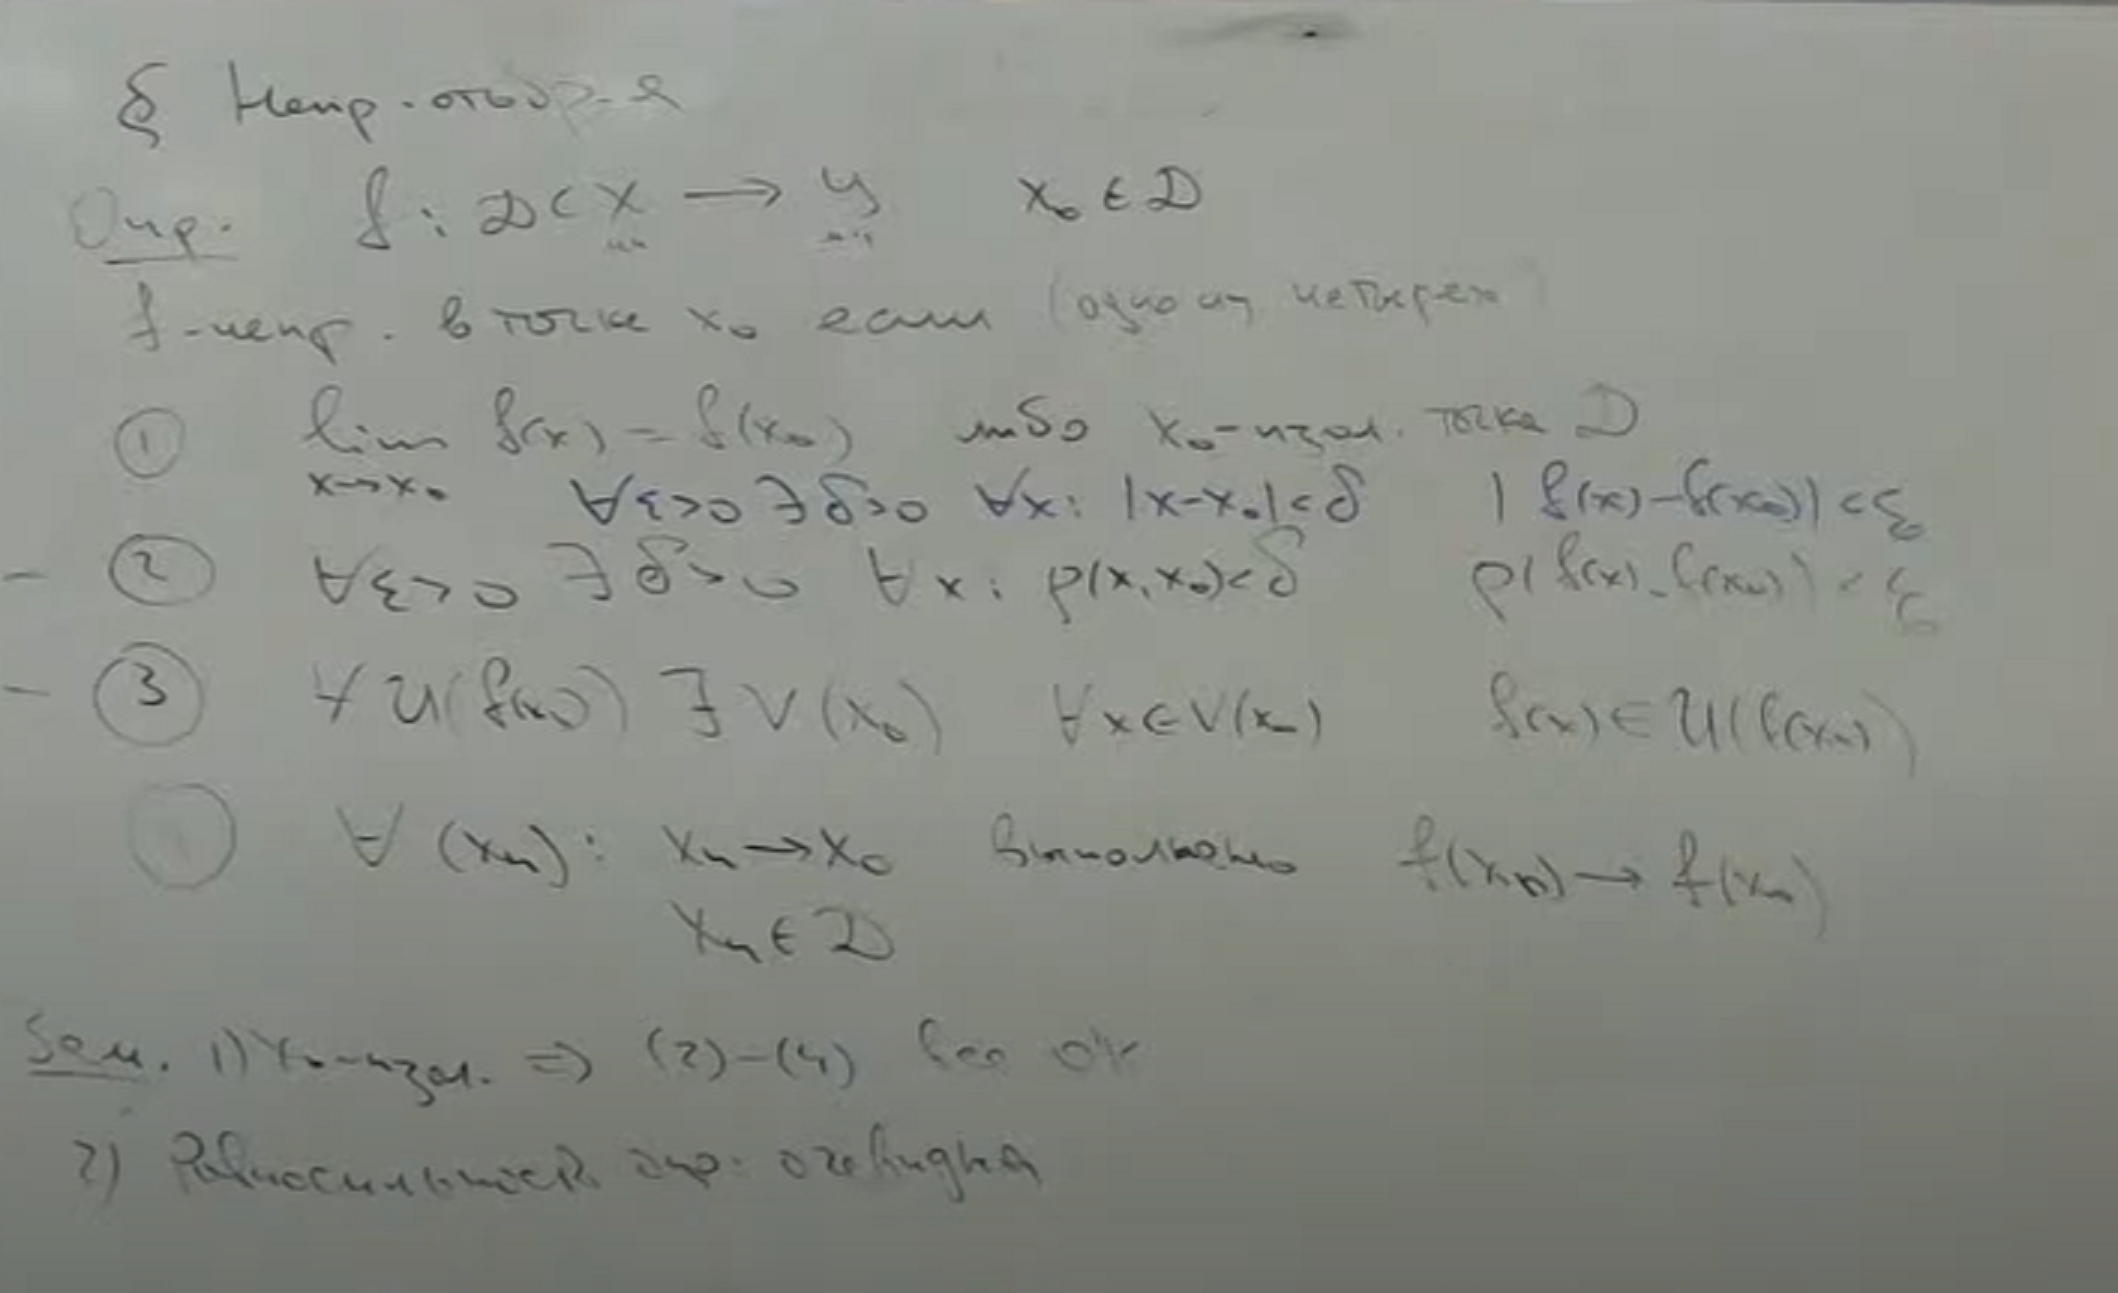
\includegraphics[scale=0.4]{Images/непрерывн отобр.png}

\newpage
\rhead{Галибов}
\subsection{Непрерывность слева}

Пусть Y — метрическое пространство, $f : D \subset \R \to Y$, $x_0 \in D$. Если сужение отображения $f$ на множество 
% Кохась брал x_0 не включительно в Е_1 и Е_2
$E_1 = D \cap (- \infty,x_0]$, $(E_2 = D \cap [x_0,+\infty))$ непрерывно в точке $x_0$, то говорят, что отображение $f$ непрерывно слева (справа) в точке $x_0$.

\newpage
\subsection{Разрыв, разрывы первого и второго рода}
% можно было бы и по-конкретнее
Разрыв. Точки, в которых нарушается условие непрерывности, называют точками разрыва функции.\\
% не порядка, а рода...
Разрыв 1 порядка. Точка разрыва $x_0$ называется точкой разрыва первого порядка, если существуют
% и f(x_0) тоже существует, но не все равны - вот тогда разрыв первого рода
конечные односторонние пределы в этой точке.\\

Разрыв 2 порядка. Точка $x_0$ называется точкой разрыва второго порядка, если она не является точкой разрыва первого рода (если хотя бы один из односторонних пределов не существует или равен +$\infty$ или $-\infty$.

\newpage
\subsection{О большое}

Пусть Х - метрическое пространство, $D \subset X$, $f,g: D \to \R(\C)$, $x_0$ - предельная точка D. Если существует функция $\phi$ : $D \to \R(\C)$ и окрестность $V_{x_0}$ точки $x_0$, такие, что $f(x) = \phi(x)g(x)$ для всех 
% проколоть окрестность надо
$x \in V_{x_0} \cap D$.\\
% а О где???
$\phi$ ограничена на $V_{x_0} \cap D$, то  говорят, что функция $f$ ограничена по сравнению с $g$ при $x \to x_0$. 

\newpage
\subsection{о маленькое}

Пусть Х - метрическое пространство, $D \subset X$, $f,g: D \to \R(\C)$, $x_0$ - предельная точка D. Если существует функция $\phi$ : $D \to \R(\C)$ и окрестность $V_{x_0}$ точки $x_0$, такие, что $f(x) = \phi(x)g(x)$ для всех 
% проколоть окрестность надо
$x \in V_{x_0} \cap D$.\\
% а о где???????????????????
$\phi \to 0$, то  говорят, что функция $f$ беконечная малая по сравнению с $g$ при $x \to x_0$. 

\newpage
\subsection{Эквивалентные функции, таблица эквивалентных}

Пусть Х - метрическое пространство, $D \subset X$, $f,g: D \to \R(\C)$, $x_0$ - предельная точка D. Если существует функция $\phi$ : $D \to \R(\C)$ и окрестность $V_{x_0}$ точки $x_0$, такие, что $f(x) = \phi(x)g(x)$ для всех 
% проколоть окрестность надо
$x \in V_{x_0} \cap D$.\\

$\phi \to 1$, то  говорят, что функция $f$ и $g$ эквивалентны при $x \to x_0$.\\
% подпиши, что это таблица эквивалентных
% эквивалентность обозначается так: ~
% не указано, что это при х -> 0
% не хваает функций - Кохась давал больше
$\sin(x) \approx \arcsin(x) \approx \tan(x) \approx \arctan(x) \approx e^x - 1 \approx x$

\newpage
\rhead{Хакимов}
\subsection{Асимптотически равные (сравнимые) функции}

\textbf{Определение.} Если $f(x) = O(g(x))$ и $g(x) = O(f(x))$ (при $x \to x_0$ или $x \in D$), то говорят, что функции $f$ и $g$ \textit{сравнимы}(при $x \to x_0$ 
% должно быть "или на мн-ве" - то, что у тебя, не имеет смысла
или $x \in D$ соответственно), и пишут $f \asymp g$

\subsection{Асимптотическое разложение}
\textbf{Определение.} 
Пусть $X$--метрическое пространство, $D \subset X,\ x_0$--предельная точка $D$, $f: D \to \R$ или $\C$ и задана
% зачем ты их перечислял?.. конечная или счетная или бесконечная - а бывают какие-то еще?
%%%%% перечисление не трудно убрать, но с ним думаю более понятнее
% а разве может быть бесконечная шкала разложения? Кохась давал так, что вроде конечная...

конечная или счётная система функций $ \{g_k\}_{k=0}^N\ (N \in \N)$ или $\{g_k\}_{k=0}^{\infty},\ g_k:\ D \to \R$ или $ \C$, каждая из которых бесконечно мала по сравнению с предыдущей при всех $k \in 
% это не прога - тут индексация с 1. 
%%%%% А в чём разница индексации с 0 и с 1???
[0: N-1] $ или $k \in \Z_{+}$ 
$$g_{k+1}(x) = o(g_k(x)),\ x\to x_0.$$
% нигде не сказано про то, что должна существовать окрестность х_0, в которой все g будут ненулевыми
%%%%% а почему нужно это указать?
Большую роль в анализе играют асимптотические формулы вида $$f(x) = \sum_{k=0}^n c_kg_k(x) + o(g_n(x)),\ \ x \to x_0.$$
Это и есть асимптотическое разложение по заданной системе функций.

\subsection{Наклонная асимптота графика}
\textbf{Определение.} Пусть $\langle a, +\infty) \subset D \subset \R,\ f: D \to \R,\ A,\ B \in \R.$ Прямая 

$y = ax+b$ называется \textit{наклонной асимптотой} графика функции $f$ при $x \to +\infty,$ если $$f(x) = A x + B + o(1),\ \ \ x\to+\infty.$$

\subsection{Путь в метрическом пространстве}
\textbf{Определение.} Пусть $Y$--метрическое пространство, $E \subset Y.$ Непрерывное отображение отрезка в множество $E$:

$$\gamma \ : [a, b] \subset \R \to E$$
называется \textit{путём} в $E$. Точка $\gamma(a)$ называется началом, $\gamma(b)$ -- концом пути.
\subsection{Линейно связное множество}
\textbf{Определение.} Пусть $Y$--метрическое пространство, $E \subset Y.$ Множество $E$ называется \textit{линейно связным}, если любые две его точки можно соединить путём в $E$: $$\forall A, B \in E,\ \exists\gamma \ : [a, b] \subset \R \to E\ :\ \gamma(a) = A,\ \gamma(b) = B.$$
\newpage
\rhead{Дзестелов}
\subsection{Счетное множество, эквивалентные множества}
\begin{definition}
    Множества $A$ и $B$ называют эквивалентными или равномощными, если между ними есть биекция, т. е. если между ними можно установить взаимооднозначное соответствие.
\end{definition}
\begin{definition}
 $A$ --- \textbf{счётное множество} $\Leftrightarrow$ равномощно/эквивалентно $\N$
\end{definition}

 %С Виноградов стр 35
\newpage
\subsection{Множество мощности континуума}
\begin{definition}
  $A$ --- \textbf{множество мощности континуума} $\Leftrightarrow$ равномощно/эквивалентно $[0; 1]$ из $\R$.
\end{definition}
\begin{consequence}
    $\R^m, m \in \N$, "$\R^\infty$" {---} континуум (под $\R^\infty$ понимается все возможные последовательности, состоящие из чисел $\R$).
\end{consequence}
\begin{remark}
    На самом деле, обобщение континууальности на размерности $\R$ напрямую следует из того факта, что $\R \Leftrightarrow [0; 1] \Leftrightarrow \operatorname{Bin}$ {---} множеству бинарных последовательностей. А т. к. декартово произведение двух последовательностей можно представить как последовательность, где на нечетных местах стоят элементы первой последовательности, а на четных элементы второй последовательности, то $\R^m$ для натуральных $m$ тоже континууально.
\end{remark}

\newpage
\subsection{Функция, дифференцируемая в точке}
% что такое ваша производная? где мои 2 нормальных определения?!
% поправил
Пусть $f: <a, b> \rightarrow \R, x_0 \in (a, b)$, тогда имеют место быть два эквивалентных определения:
\begin{definition}
Если $\exists A \in \R: f(x) = f(x_0) + A(x - x_0) + o(x - x_0), x \rightarrow x_0$, тогда $f$ - дифф. в $x_0$, а $A$ - производная в этой точке.
\end{definition}
\begin{definition}
Если $\exists \lim\limits_{h \to 0} \frac{f(x+h)-f(x)}{h} = A \in \R$, где $h = x - x_0$, тогда $f$ - дифф. в $x_0$, а $A$ - производная в этой точке. 
\end{definition}
\begin{remark}
    Функция, дифференцируемая в точке - это функция, которая имеет конечную производную в точке. На самом деле, функция может иметь бесконечную производную, тогда фактически говорят о наличии производной, однако не считают функцию дифференцируемой в этой точке.
\end{remark}

\newpage
\subsection{Производная}
\begin{definition}
Пусть $f: D \rightarrow \R, D_1 \in D$ {---} множество точек дифференцирования, тогда производной называется функция:
$$ \phi:\ D_1 \xrightarrow[x \mapsto f'(x)]{} \R: f(x) = f(x_0) + A(x - x_0) + o(x - x_0),\ x \rightarrow x_0$$
\end{definition}
 
\newpage
\subsection{Касательная прямая к графику функции}
\begin{definition}
Касательной к графику функции $f(x), f(x)$ {---} определена и дифф. в некоторой окрестности точки $x_0$, называется прямая $y = f(x_0) + f'(x_0)(x - x_0)$.
\end{definition}
\begin{remark}
По второму определению производной угловой коэффицент касательной равен пределу угловых коэффицентов секущих.    
\end{remark}

\newpage
\rhead{Шехунов}
\subsection{Классы функций $C^n([a,b])$}
\textbf{Определение гладкой функции} \\\\
\textbf{Гладкая функция} — функция имеющая непрерывную производную на всем множестве определения. \\\\
Рассматривают также гладкие функции высших порядков, а именно, функция с порядком гладкости $\mathbf{r}$ имеет непрерывную производную порядка $\mathbf{r}$. \\
Множество таких функций, определённых в области $\mathbf{\Omega}$ обозначается $\mathbf{C^{r}(\Omega)}$ \\
$\mathbf{f \in C^{\infty}(\Omega)}$ означает, что $\mathbf{\forall r \in \mathbb{N} : f \in C^{r}(\Omega)}$ \\\\
\newpage

% почему в определении так мало сказано про саму функцию f?
% Вроде поправил
\subsection{Производная n-го порядка}
$\mathbf{X, Y}$ - произвольные метрические пространства \\
Пусть функция $\mathbf{f : X \rightarrow Y}$ имеет конечную производную $\mathbf{f'(x)}$ в некотором интервале $(a, b)$, $\mathbf{f'(x)}$ так же является функцией в этом интервале, если она дифференцируема, то мы так же можем вычислить от неё проивзодную: 
$\mathbf{f''(x) = (f'(x))' = ((\frac{dy}{dx})' = \frac{d^{2}y}{dx^{2}}}$ \\
$\mathbf{f''(x)}$ так же обозночается как $\mathbf{f^{(2)}(x)}$ и называется производной второго порядка. \\ Аналогично мы можем вычислить производную третьего, четвертого \dots 
 порядков. \\\\
Таким образом понятие \textbf{производной n-го} порядка вводится индуктивно, через последовательное вычисление $n$ производных, начиная с производной 1-го порядка.

\newpage 
\subsection{Многочлен Тейлора n-го порядка}
Пусть функция $\mathbf{f(x)}$ определена в некоторой окрестности точки $x_0$ и $n$ раз дифференцируема в точке $x_0$. \\ 
Данный многочлен называется многочленом Тейлора n-го порядка функции $\mathbf{f(x)}$ в точке $\mathbf{x_0}$: 
% он не так у Кохася обозначается...
$$\mathbf{P(x) = \sum_{k=0}^{n} \frac{f^{(k)}(x_0)}{k!} (x-x_0)^{k}}$$ 

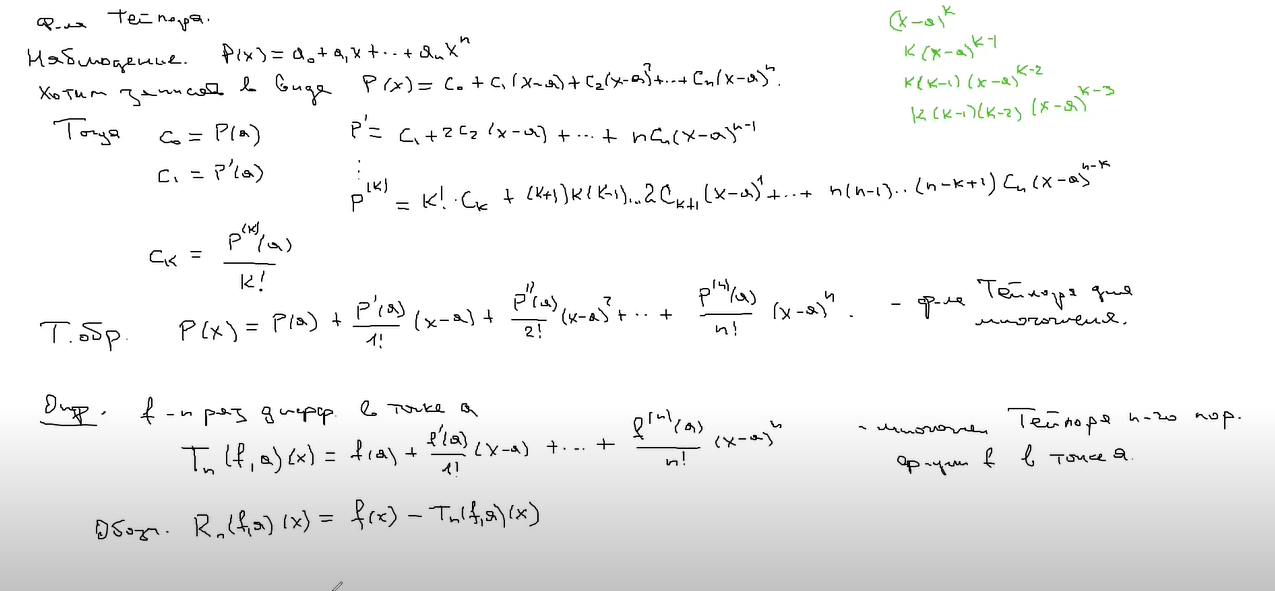
\includegraphics[scale=0.65]{Images/многочлен_Тейлора.png}

\newpage
\subsection{Разложения Тейлора основных элементарных функций}
что то \\
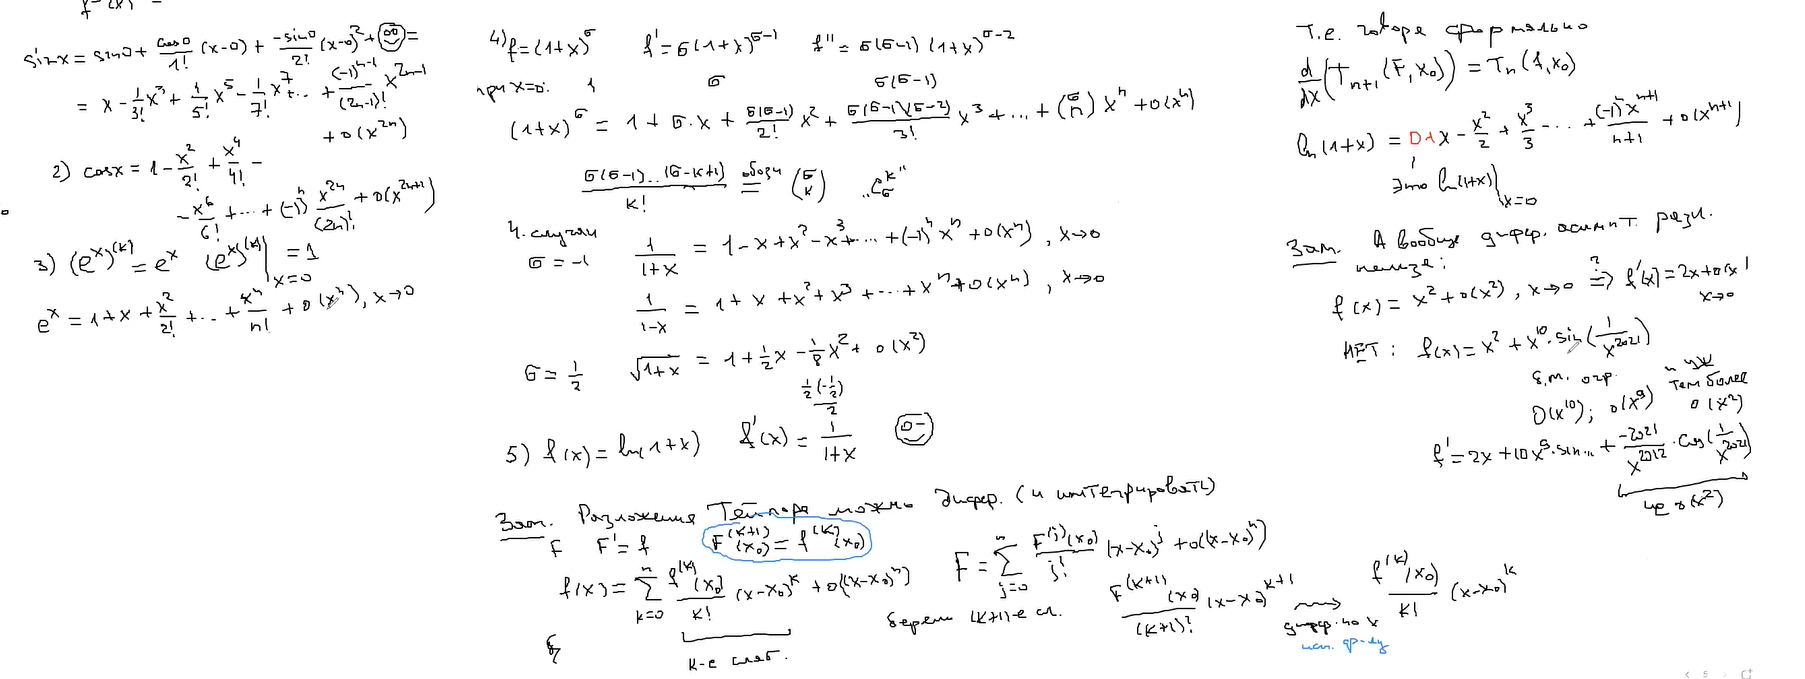
\includegraphics[scale=0.5]{Images/элеменфункц.png}

\end{document}
 